\documentclass{article}
\usepackage{iclr2027_conference,times}
\iclrfinalcopy
\usepackage[utf8]{inputenc}
\usepackage[T1]{fontenc}
\usepackage[expansion=false,protrusion=true]{microtype}
\usepackage{amsmath,amssymb,amsthm}
\newtheorem{proposition}{Proposition}
\usepackage{graphicx}
\usepackage{booktabs}
\usepackage{multirow}
\usepackage{xcolor}
\usepackage{hyperref}
\hypersetup{hidelinks}
\usepackage[capitalize,noabbrev]{cleveref}
\usepackage{caption}
\usepackage{subcaption}
\usepackage{xspace}
\usepackage{enumitem}
\usepackage{mdframed}
\newmdenv[
  linewidth=0.4pt,
  linecolor=blue!40,
  backgroundcolor=blue!4,
  innerleftmargin=6pt,
  innerrightmargin=6pt,
  innertopmargin=3pt,
  innerbottommargin=3pt,
  skipabove=3pt,
  skipbelow=3pt,
]{takeaway}

\newcommand{\todo}[1]{\textcolor{red}{\textbf{[TODO: #1]}}}
\newcommand{\tbd}{\textcolor{purple}{\underline{v1}}}
\newcommand{\placeholder}[1]{\textcolor{purple}{\underline{#1}}}
\newcommand{\pred}[1]{\textcolor{purple}{\underline{#1}}}

\newcommand{\circuittracer}{\texttt{circuit-tracer}\xspace}
\newcommand{\jaccard}{\operatorname{Jaccard}}
\newcommand{\qwen}[1]{Qwen3\if\relax\detokenize{#1}\relax\else-#1\fi}
\newcommand{\gemma}[1]{Gemma3\if\relax\detokenize{#1}\relax\else-#1\fi}

\title{Cross-Model SAE Coactivation Survives\\Length, Topic, and Lexical Controls}

\author{Xupeng Chen$^{1,*}$ \quad Runhao Li$^{2}$ \quad Jiayi Cheng$^{1}$ \quad Michael Yue$^{3}$ \quad Chenqian Le$^{1}$ \\
{\normalfont $^{1}$New York University \quad $^{2}$University of Southern California \quad $^{3}$Columbia University} \\
{\normalfont $^{*}$Corresponding author: \texttt{xc1490@nyu.edu}}}

\date{}

\newcommand{\coderepo}{\url{https://github.com/james20141606/cross-model-sae-coactivation}}
\begin{document}
\maketitle
\lhead{Preprint}

\begin{abstract}
Cross-model matches of sparse-autoencoder (SAE) features have been judged against random
pairings or neuron baselines, neither of which re-runs the pairing rule. Gemma-2-9B and Mistral-7B,
from different families with different tokenizers, each have a released-SAE obituary feature, and
the two share their top five documents: is it the same feature? Our controls support a more specific answer: matched features of these two models respond
to the same inputs beyond chance and pair selection, and that shared response survives the topic
and vocabulary controls we ran; this is coactivation, not feature identity. Such matches are cheap: two sets of
$1{,}500$ features reciprocally match about half of each other under idealized chance, and any
document property both models encode (length, topic, vocabulary) can make features coactivate. We
run the pairing rule inside a document-permutation null, score frozen pairs on documents the
rule never saw, and add controls that each fix one named nuisance. In a
non-pre-registered follow-up, all nine cross-family cells (Gemma-2, Mistral, Qwen3, Llama-3)
hold on disjoint C4 text ($p=1/2001$ each, Bonferroni over the 17-cell roster). The sharing
survives length- and coarse topic-matched nulls (one cell); on three representative
cells, every control leaves at least $0.88$ of the excess its reference arm leaves. Regressing out a unigram TF-IDF
lexical model, which a pre-registered gate shows is not inert, leaves $92$--$94\%$ of the
excess: the shared-vocabulary explanation is narrowed, not closed. A registered token-aligned
test shows the sharing is not reducible to document means (it beats a within-document
word-order shuffle; mean pair correlation $0.522$/$0.398$/$0.335$) and, in a leakage-clean design, keeps
$R_{\text{tok}}^{\text{clean}}{=}0.925$--$0.986$ of its token-level excess after conditioning on
the document and the current word. The claim does not extend to compositional or syntactic
sharing, a capability trend (swapping only one model's SAE width
moves its cell from $z=22.1$ to $14.1$), or shared computation (both cross-model
ablation probes were inconclusive). The controls can say no: they rejected three decisive-looking
secondary results, all reported (a cross-lingual metric that tracks network depth rather than
language, its depth-corrected residual, and a Pythia-70M$\leftrightarrow$Mistral-7B match null on natural text).
Cross-model matches should be scored against a null that re-runs the matching, on documents
the matching never saw, one nuisance per control; code, nulls, receipts and
registrations are released at \coderepo.

\end{abstract}

\section{Introduction}\label{sec:intro}

Feature-universality studies pair sparse-autoencoder (SAE) features of separately trained
networks by their highest activation correlation
\citep{bricken2023monosemanticity,wang2025universality,lan2024universal}, and read close pairs as evidence of shared features.
On C4, the released SAEs of Gemma-2-9B and Mistral-7B, two families with different tokenizers,
each have an obituary feature, and the two features' five most-activating documents are the same five (\Cref{app:matched-examples}). Such pairs are cheap to manufacture: two sets of $1{,}500$ features
reciprocally match about half of each other under idealized chance (\Cref{prop:null}), and any
document property both models encode (length, topic, vocabulary, the current word) can make
features coactivate with no shared feature behind them.

\begin{figure}[t]
\centering
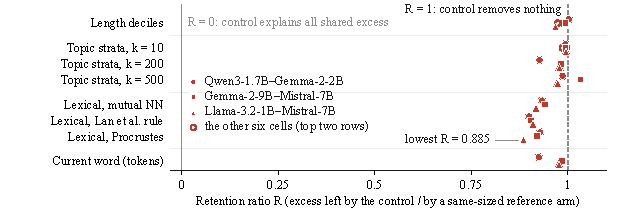
\includegraphics[width=\textwidth]{figures/fig1_20261010/fig1.pdf}
\caption{\textbf{Every control we ran leaves nearly all of the cross-model shared excess: retention ratios sit near $R=1$, far from $R=0$.} $R$ \eqref{eq:ratio} is the excess left after a control over that left by a same-sized reference arm; $R=1$ means the control removes nothing beyond its reference arm, and $R=0$ that the covariate, as the control captures it, explains all of the sharing. Top two rows: all nine cross-family cells (\Cref{tab:ninecell}); other rows: three representative cells (\Cref{tab:ladder}). Drawn by \texttt{code/figures/fig1\_control\_ladder\_20261010.py} from the \texttt{ninecell\_20260926/A\_*}, \texttt{lextok20k\_*}, \texttt{lanpair\_*}, \texttt{proclex\_*} and \texttt{tokaclean20k\_*} receipts.}
\label{fig:arc}\label{fig:controls-main}
\end{figure}

Sparse autoencoders and transcoders \citep{cunningham2023sparse,bricken2023monosemanticity,
ameisen2025attribution,lindsey2025biology} make such comparisons easy to run, and cross-model
matches are read as evidence of representational convergence
\citep{huh2024platonic,lan2024universal}. The published cross-model protocol pairs features
greedily and judges significance against random pairings, on same-tokenizer pairs and without
controls for shared document properties \citep{lan2024universal}. A pairing rule fit to the data inflates any statistic
computed on the same data \citep{kriegeskorte2009circular}: re-implemented without their
filters on three of our pairs (all but GPT-2$\leftrightarrow$Mistral-7B, which shows no signal above random), a null that permutes documents before the pairing step sits far above that random
baseline, so part of the signal above random (up to $94\%$ on templated prompts, less on C4) comes
from the pairing itself (\Cref{app:lan}). With their filters added, that share shrinks on templates
but does not vanish, and on C4 too few permuted pairs survive the filters to estimate it
(\Cref{app:lan_filters}). That protocol lacks a null that re-runs the pairing
rule, pairs scored on documents the rule never saw, and controls that hold named mundane causes fixed.

We add all three, on open-weight models, and apply controls built to kill the signal
(\Cref{fig:arc}). It survives. In all nine cross-family cells across Gemma-2, Mistral, Qwen3
and Llama-3, pairs selected on half of a C4 slice still beat their null on the disjoint other
half (each at the floor of its permutation test; this follow-up was not pre-registered). On three representative
cells, fine topic strata, cross-fitted lexical residualization under three pairing rules, and
registered current-word conditioning at token level each leave a retention ratio of at least
$0.88$ against its reference arm. What survives is coactivation on shared inputs, not feature
identity: both cross-model ablation probes were inconclusive, and a dictionary confound (cells differ
in SAE dictionary, not only in model) blocks any capability-trend reading. The instruments
behind the positive can return a no: size- and sparsity-matched random directions fall below
their own null, Pythia-70M$\leftrightarrow$Mistral-7B falls to null on C4, and on
planted data the token-aligned analysis collapses a unigram-only signal while planted context
survives (\Cref{app:tokalign}).

\paragraph{Contributions.}
\begin{enumerate}[leftmargin=*,topsep=2pt,itemsep=1pt]
  \item \textbf{A reusable test that separates shared responses from named mundane correlates.} A
  re-matching permutation null, frozen pairs scored on disjoint documents, and controls read as retention
  ratios against a same-sized reference arm; two propositions show why, for any pairing rule, the null and
  frozen score carry no selection optimism while a re-selected score does (\Cref{sec:method}).
  \item \textbf{A scoped cross-model positive.} Coactivation on shared inputs in nine
  cross-family cells on held-out documents (non-pre-registered), three of them through the full control ladder (\Cref{fig:arc,fig:heldout-main},
  \Cref{tab:ladder}); not feature identity, composition, a capability trend, or shared computation.
  \item \textbf{Three rejections, each with the practice it implies.} The controls reject a
  Pythia-70M$\leftrightarrow$Mistral-7B match null on natural text (so recheck template matches on
  natural text), a depth-driven cross-lingual metric (so add a mismatched-concept control), and its
  depth-corrected residual at $206$ concept pairs and $17$ models (so use several English-only
  baselines) (\Cref{sec:results:secondary,sec:results:sae-matching}).
\end{enumerate}

\section{Related Work}\label{sec:related}

\paragraph{Sparse dictionaries and attribution graphs.}
Sparse autoencoders decompose residual streams into more monosemantic features
\citep{cunningham2023sparse,bricken2023monosemanticity,rajamanoharan2024gated,templeton2024scaling};
transcoders and cross-layer transcoders predict across layers so that direct linear effects
can be computed, and \circuittracer{} turns them into attribution graphs
\citep{ameisen2025attribution,lindsey2025biology,hanna2025circuit-tracer}. Released
dictionaries now exist for Gemma-2, Gemma-3 and Qwen3
\citep{lieberum2024gemmascope,mcdougall2025gemmascope2,hanna2025qwen-transcoders,bluelightai2025qwen-clt},
with \circuittracer{} configurations for the Gemma-3 transcoders \citep{hanna2025gemma-scope-2-transcoders}.
We train no dictionary: every claim attaches to a (model, released SAE) pair, which is what a
practitioner reusing these artifacts would compare.

\paragraph{Convergent units and convergent geometry.}
Bipartite unit matching across independently trained vision networks began with convergent
learning \citep{li2016convergent}; Rosetta neurons recur across vision models
\citep{dravid2023rosetta}, with counts that grow sublinearly in scale \citep{dravid2026divergent},
and only a small fraction of GPT-2 neurons are universal \citep{gurnee2024universal}. At the level
of global geometry, \citet{huh2024platonic} argue that capable models converge, while
\citet{groger2026aristotelian} show that such similarity scores are confounded by scale, and that after
permutation calibration the convergence seen by global spectral measures largely disappears while
local-neighborhood similarity retains significant agreement. Circuit-level recurrence is
documented for vision circuits, induction heads and toy tasks
\citep{olah2020zoom,olsson2022context,chughtai2023toy}, while behavior tied to a single concept
can still differ by family \citep{soligo2026distress}. These works ask whether units or geometries recur; we
ask a narrower question: do post-hoc features of LMs with different tokenizers respond to
the same documents once named document covariates are held fixed?

\paragraph{Matching or mapping features across models.}
\citet{bricken2023monosemanticity} match features across seeds by activation correlation, and
\citet{lan2024universal} pair features across models and compare the paired decoder spaces with
SVCCA/RSA \citep{raghu2017svcca,kriegeskorte2008rsa} against random pairings.
\citet{wang2025universality} match SAE features of Pythia-160M and Mamba-130M, which share a
tokenizer and training corpus, by maximum pairwise correlation over tokens, and read the result
against a neuron baseline and seed-variant skylines rather than a null that re-runs the matching. Crosscoders and
universal SAEs instead learn a shared dictionary during training
\citep{lindsey2024crosscoders,thasarathan2025usae}, and their shared/exclusive diagnostic needs its
own correction \citep{minder2025crosscoder}. A third line connects models through learned maps:
stitching \citep{bansal2021stitching}, permutation re-basin \citep{ainsworth2023rebasin}, and affine
residual maps that carry SAEs, probes and steering vectors
\citep{chen2025stitching,huang2025platonictransfer}, with success depending on scale and
tokenizer overlap \citep{gorbett2026linear}; steering vectors also transfer across architectures
through learned nonlinear bridges between the models' SAE feature spaces
\citep{agarwal2026crossarch}, and relative representations avoid a learned map
altogether \citep{moschella2023relative}. A learned map can succeed without any shared sparse
feature, and a pairing rule fit to the data inflates any statistic computed on the same data. We
therefore use no learned map in the headline, put the pairing rule inside the null, and score
frozen pairs on documents the rule never saw. SVCCA/RSA appear only in our audit of
\citet{lan2024universal} (\Cref{app:lan}): a global score cannot say which features correspond, and
a crosscoder's shared latents would need retraining for every null draw (\Cref{app:failure_methods}).

\paragraph{Cross-lingual mechanisms.}
\citet{templeton2024scaling} report SAE features that fire across languages in Claude 3 Sonnet,
and \citet{lindsey2025biology} extend this to circuits in Claude 3.5 Haiku; both are closed-weight.
In open models, logit-lens decoding suggests an English-centered latent
\citep{wendler2024llamaspeak}, some SAE features are language-specific in that ablating them harms
one language \citep{deng2025languagespecific}, answer consistency comes apart from representation
sharing \citep{ifergan2024beneath}, sharing depends on model and architecture
\citep{bogdanov2026geoinv}, and mid-layer overlap within Gemma-2 is reported by
\citet{son2025semanticconvergence}. We reuse this question in open weights mainly as a test case
for the control battery, not as the headline.

\paragraph{Construct validity and circular analysis.}
Representational-similarity metrics can be high for reasons unrelated to what they claim to
measure \citep[surveyed by][]{klabunde2023similarity}: \citet{ding2021grounding} ask for
sensitivity and specificity and show that CKA and CCA \citep{kornblith2019cka} can fail them,
\citet{davari2023reliability} show CKA can be manipulated without changing model function,
\citet{korznikov2026sanity} find random directions rivalling trained SAE features, and SAEs on
randomly initialized transformers can match trained ones on common interpretability metrics
\citep{heap2025random}. Scoring a
selection on the data that made it is the circular analysis of
\citet{kriegeskorte2009circular}; plus-one permutation $p$-values are the standard fix for
Monte-Carlo nulls \citep{phipson2010permutation}. We carry both into feature matching: a count is
read only against a null that re-runs its own selection, and then against nulls that hold named
covariates fixed.

\section{Problem Setup}\label{sec:method}

To tell a match like the obituary pair from chance and from shared document properties, the
statistic needs a known chance level, a null that re-runs its own selection, and controls read
against a reference arm.

\paragraph{Coactivation.} Let $A$ and $B$ be two models, each with one released SAE at a
mid-layer residual site, and $D=\{d_1,\dots,d_N\}$ a shared corpus. For feature $i$ of $A$'s SAE,
$f^A_i(d)$ is its activation mean-pooled over $A$'s tokens of document $d$, one scalar per
(document, feature), which sidesteps the tokenizer mismatch. We keep the $K{=}1{,}500$
highest-variance features per model, standardize each over $D$ to $z^A_i(d)$, and define
\begin{equation}\label{eq:rho}
\rho_{ij} \;=\; \tfrac{1}{N}\textstyle\sum_{n=1}^{N} z^A_i(d_n)\, z^B_j(d_n),
\qquad i\le K_A,\; j\le K_B,
\end{equation}
the correlation of the two features across documents. Here ``sharing'' denotes residual dependence in $\rho$
under the tested controls; it is not feature identity and not shared computation.

\paragraph{Reciprocal matching and its null.} With $a(i)=\arg\max_j\rho_{ij}$ and
$b(j)=\arg\max_i\rho_{ij}$, the reciprocal (mutual-nearest-neighbor) pairs and their count are
\begin{equation}\label{eq:count}
\mathcal{M}(\rho)=\{(i,j):a(i)=j,\ b(j)=i\},\qquad M=|\mathcal{M}(\rho)|.
\end{equation}
The null permutes documents on one side: for $\pi$ uniform on $S_N$, $\rho^{\pi}$ is
\eqref{eq:rho} with $z^B_j(d_{\pi(n)})$, and $M^{\pi}=|\mathcal{M}(\rho^{\pi})|$ \emph{re-runs the
matching}. From draws $M^{(1)},\dots,M^{(n_{\text{perm}})}$ we report
\begin{equation}\label{eq:excess}
\Delta = M-\overline{M^{\pi}},\qquad z=\Delta/\operatorname{sd}(M^{\pi}),\qquad
p=\frac{1+\#\{b: M^{(b)}\ge M\}}{n_{\text{perm}}+1}.
\end{equation}
Significance rests on $p$ \citep{phipson2010permutation}, never on a Gaussian reading of $z$.
Two facts fix the design (proofs in \Cref{app:proofs}).

\begin{proposition}[Chance reciprocal matches; validity of the re-matching null]\label{prop:null}
(a) If, for every $(i,j)$, the $K_A{+}K_B{-}1$ entries in row $i$ and column $j$ of $\rho$ are
exchangeable and almost surely distinct (e.g.\ i.i.d.\ continuous), then
$\mathbb{E}[M]=K_AK_B/(K_A{+}K_B{-}1)$, i.e.\ $\approx750$ at $K_A{=}K_B{=}1{,}500$.
(b) Permuting documents on one side leaves both within-model correlation matrices unchanged.
If $H_0$ holds, i.e.\ $(z^A,z^B)\overset{d}{=}(z^A,z^B\!\circ\pi)$ for every $\pi\in S_N$, then
every statistic of $(z^A,z^B)$, including one that selects its own pairs, has
$\Pr(p\le\alpha)\le\alpha$ for all $\alpha$.
\end{proposition}

By (a), about half of the $1{,}500$ screened features per model are reciprocally matched under
idealized chance, more than
the raw count of our weakest surviving cell (\Cref{tab:ladder}); the realized chance level also
depends on each dictionary's internal correlations, which the null preserves, so every cell gets
its own null and $z$ is never compared across cells. By (b), rejecting $H_0$ shows dependence
between the models on shared documents, not correspondence: any document property both models
encode (length, topic, vocabulary) also violates $H_0$. That is what the controls are for.

\paragraph{Held-out frozen pairs.} Split the corpus into disjoint halves $D_S,D_E$ ($1{,}000$
C4 documents each). Pairs $\widehat{\mathcal{P}}=\mathcal{M}(\rho^{S})$ selected on $D_S$ are
frozen and scored on $D_E$ by $T_E(\mathcal{P})=|\mathcal{P}|^{-1}\sum_{(i,j)\in\mathcal{P}}\rho^{E}_{ij}$,
with excess $\Delta_E$ and $p$ from $2{,}000$ permutations of $D_E$ alone. The ratio
$r=\Delta_E(\widehat{\mathcal{P}})/\Delta_E(\mathcal{M}(\rho^{E}))$ compares against pairs
re-selected on $D_E$, a different pair set, so it is not within-pair retention.

\begin{proposition}[Frozen pairs carry no selection optimism]\label{prop:heldout}
Let documents be i.i.d., $D_S\cap D_E=\emptyset$, and $\widehat{\mathcal{P}}$ depend on $D_S$
only. Conditional on $D_S$: (a)
$\mathbb{E}[T_E(\widehat{\mathcal{P}})\mid D_S]=|\widehat{\mathcal{P}}|^{-1}
\sum_{(i,j)\in\widehat{\mathcal{P}}}\mathbb{E}[\rho^E_{ij}]$, as for a pair set fixed in advance;
(b) the permutation $p$ on $D_E$ is valid under $H_0$ restricted to $D_E$. Pairs re-selected on
$D_E$ and held fixed in the null, as in the denominator of $r$, need not have either property:
$\mathbb{E}[\max_j\rho^E_{ij}]\ge\max_j\mathbb{E}[\rho^E_{ij}]$; re-selecting in every draw
restores (b) by \Cref{prop:null}(b).
\end{proposition}

This is what lets the nine held-out cells carry the positive, conditional on its i.i.d. premise:
our C4 slice is the first $2{,}000$ eligible streamed documents, split into consecutive halves. On five
cells, seeded random halves change the median held-out excess by at most $3\%$ (separately extracted features,
\Cref{app:ninecell}); on the three ladder cells, a seeded random split of $20{,}000$ documents keeps
$0.97$--$0.99$ of in-sample excess held out (\Cref{app:threats}); the Qwen3-8B cells were untested at
submission (a registered run after submission covers all nine, \Cref{app:ninecell}). The follow-up was not
pre-registered, and its screen saw both halves (\Cref{tab:c4_verdicts}).

\paragraph{Controls as retention ratios.} A control either restricts $\pi$ to permutations
within strata of a covariate (valid under within-stratum exchangeability) or removes the
covariate from the features before frozen pairs are scored. Removing \emph{anything} costs excess
mechanically, so each control is divided by a reference arm: a same-sized transformation that
carries no information about the covariate or, for tokens, the unconditioned statistic on the
same occurrences. We report
\begin{equation}\label{eq:ratio}
R=\Delta_{\text{control}}\,/\,\Delta_{\text{calibration}},
\end{equation}
so $R\approx1$ means the covariate, as the control captures it, explains none of the shared
excess and $R\to0$ all of it; forms of the covariate the control does not capture are not excluded.
Instances: $k$-way TF-IDF topic strata vs.\ random strata of identical sizes ($R$);
cross-fitted residualization on a TF-IDF$\to$SVD$_k$ design vs.\ a row-shuffled design of
identical spectrum ($R_{\text{lex}}$); and, at word granularity, document plus word-type fixed
effects vs.\ a within-type derangement ($R_{\text{tok}}$: conditioned over unconditioned
token-level excess on common support). The secondary cross-lingual measure, probe-attribution
alignment (mid-layer logit-lens profiles correlated across translated prompts), is defined in
\Cref{app:probe_attribution}. Neither uses attribution-graph topology, which our v0
pipeline did not recover (\Cref{sec:disc:negative}).

\section{Experimental Setup}\label{sec:experiments}

\paragraph{Models, prompts, and compute.} Two arms share one control discipline: SAE
matching across models, and cross-lingual probe attribution within them. The SAE-matching arm uses Gemma-\mbox{2-2B/9B} \citep{gemma2024gemma2}, Mistral-7B \citep{jiang2023mistral},
Qwen3-1.7B/8B-Base \citep{yang2025qwen3}, Llama-3.2-1B \citep{grattafiori2024llama3}, Pythia-70M
\citep{biderman2023pythia} and GPT-2 \citep{radford2019gpt2}, each with one released SAE
(\Cref{tab:sae-roster}), on a shared $206$-prompt English concept corpus and on C4 (each ``document'' is the first
$300$ characters of a record, so full-length documents are untested; \Cref{app:prompts}). The
probe-attribution sweep uses the eight (model, transcoder) pairs of \Cref{tab:models} plus
Gemma3-1B and Pythia (70M--1.4B), on $20$ aligned antonym pairs per language in en/zh/ja/ko,
expanded to $206$ concept pairs across nine concept families and $17$ models for the residual scale-up.
Prompt lists, target tokens and provenance are in \Cref{app:prompts}; each model scores the first
token of its own tokenization of the target. We call the abandoned attribution-graph pipeline
\emph{v0} and the functional pipeline behind every result \emph{v1}. Compute is in \Cref{app:scheduling}. Intervals are $95\%$ bootstrap
CIs ($10{,}000$ resamples; model/data seeds $0$, bootstrap seed $1$).

\paragraph{Statistical reporting.} The unit of inference is stated with each result: language
pairs (raw probe-attribution), models and pairs (residual scale-up), and (model pair, corpus)
cells (SAE matching). All $p$-values use \eqref{eq:excess}. The same-corpus $200$-draw C4 screen
is descriptive; the non-pre-registered disjoint-half follow-up uses $2{,}000$ draws and all nine
tests clear Bonferroni over the $17$ C4 cells ($1/2001<0.05/17$). Other verdicts use registered
survive/fail controls, not marginal significance; cross-lingual gradations are descriptive.

\section{Results}\label{sec:results}

\begin{figure}[t]
\centering
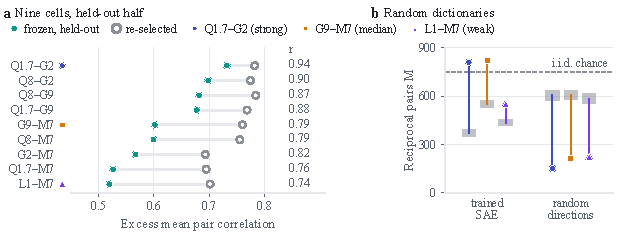
\includegraphics[width=\textwidth]{figures/results_20261010/main_results.pdf}
\caption{\textbf{The coactivation survives disjoint documents in all nine cells, and matched random directions do not reproduce it;} the control ladder is \Cref{fig:arc}, where on three representative cells every control has retention ratio $R\ge0.88$ against its reference arm, and length-decile nulls, run on six of the nine cells, leave at least $0.96$ of the excess (\Cref{app:lencov,app:ninecell}; all nine after submission). (a)~Pairs selected on $1{,}000$ C4 documents and frozen
(filled) vs.\ pairs re-selected on the evaluation half (open); $r$ is their ratio of excesses,
over two different pair sets (\Cref{prop:heldout}); every held-out $p=1/2001$. (b)~Reciprocal count $M$
(marker) against its own permutation null (grey, mean${\pm}2$\,SD) for trained SAEs and
size/sparsity-matched random directions; dashed: the i.i.d.\ chance level of
\Cref{prop:null}(a). Q/G/M/L $=$ Qwen3/Gemma-2/Mistral/Llama-3.2, number $=$ size (B). Drawn
by \texttt{code/figures/main\_results\_20261010.py} from \texttt{heldout\_*}, \texttt{c4\_*} and \texttt{rand\_c4\_*.json}.}
\label{fig:heldout-main}
\end{figure}

\subsection{Cross-model SAE feature matching}\label{sec:results:sae-matching}

We run the pipeline of \Cref{sec:method} on the pairs of \Cref{tab:sae-roster}, each model with
\emph{one} publicly released SAE (\texttt{sae-lens}, \citealp{bloom2024saelens}; Gemma Scope's is read one block
before its training hook, \Cref{app:gemmahook}) and mean-pooled features, so claims attach to
(model, SAE, read point, pooling) (\Cref{app:threats}).

\paragraph{Finding 1: the natural-text control decides which cells merit held-out testing.} On
the templated concept corpus every tested pair among Gemma-2, Mistral-7B and Pythia (models from $70$M to $9$B)
clears its reciprocal null (\Cref{tab:sae_matching}). The $2{,}000$-document C4 screen
\citep{raffel2020exploring} then separates candidates from a corpus artifact
(\Cref{tab:c4_counts}): Pythia-70M$\leftrightarrow$Mistral-7B, a cross-family cell strongly
significant on templates, \emph{falls to null on C4}; its sharing was template-tuned. The
modern ${\gtrsim}1$B pairs survive, and Qwen3-1.7B/8B (Qwen-Scope SAEs, \citealp{qwenscope2026};
manual adapter) share with both other families, as does Llama-3.2-1B
(\citealp{chanind2024llamasae}) against Mistral-7B (SAE: \citealp{engels2024mistralsae}): nine
cross-family cells across four families. In the non-pre-registered held-out follow-up, freezing
first-half pairs and scoring them on the second half confirms all nine at
$p=1/2001$, which clears Bonferroni over all $17$ C4 cells considered; held-out excess is
$74$--$94\%$ of the eval-half re-selected excess, a ratio over different pair sets, not
within-pair retention (\Cref{fig:heldout-main}a, \Cref{tab:c4_verdicts}). The templated corpus errs in both
directions: Qwen3-1.7B$\leftrightarrow$Gemma-2-2B is weak on templates ($z=3.59$, $p=1/201$) and strong on C4 ($z=42.7$), the
mirror image of the Pythia artifact, hence the natural-text headline.

\paragraph{What we do \emph{not} claim: no capability trend.} Against the fixed Mistral-7B
reference, $z$ rises with size across Pythia-70M, Llama-3.2-1B, Qwen3-1.7B, Gemma-2-2B and
Gemma-2-9B, which invites a reading as emergence with
capability and an SAE-level Platonic Representation Hypothesis \citep{huh2024platonic}. The axis
is confounded with the dictionary: these five cells pair Mistral's SAE with four other SAE suites, and
swapping only the Gemma-2-2B dictionary $16$k$\to$$65$k moves its cell from $z=22.1$ to $14.1$
with no change of model (\Cref{tab:c4_counts}). What survives is the per-cell verdict, which
needs no cross-cell comparison. GPT-2's four natural-text cells are underpowered (\Cref{app:threats}), so exactly one model is measured below null with power. On the
templated corpus both Gemma$\leftrightarrow$Mistral pairs are significant at all three depth bands
(\Cref{tab:sae_matching}); on C4 each model is read at one mid-layer hook.

\begin{table}[t]
\centering
\caption{\textbf{The control ladder: each rung is a way to explain the shared excess away, and on
three representative cells none does.} Values are
strong/median/weak (Qwen3-1.7B$\leftrightarrow$Gemma-\mbox{2-2B}, Gemma-2-9B$\leftrightarrow$Mistral-7B,
Llama-3.2-1B$\leftrightarrow$Mistral-7B). Ratios follow \eqref{eq:ratio}; lexical rows use the
governing $k{=}4096$. ``reg.'': rule and outcome branches registered before the receipt existed;
the held-out follow-up was not. Topic rows (revised after submission): the size-matched
calibration averages $20$ random partitions in the registered nine-cell run (\Cref{app:ninecell});
the submitted values used one partition (\Cref{tab:covctl}). Full tables: \Cref{tab:c4_verdicts,tab:rand_control,tab:covctl,tab:lextok,tab:lanpair,tab:proclex,tab:tokalign}.}
\label{tab:ladder}
\footnotesize
\setlength{\tabcolsep}{3pt}
\begin{tabular}{@{}lllr@{}}
\toprule
Rung & Statistic & strong/median/weak & $p$ \\
\midrule
C4 screen, $2{,}000$ docs & $M$ (null mean) & $811$ ($371.8$)/$819$ ($553.4$)/$551$ ($434.9$) & $1/201$ \\
Random directions (size, $L_0$ matched) & $M$ (null mean) & $152$ ($604.7$)/$212$ ($607.0$)/$223$ ($584.5$) & $1.0$ \\
Held-out frozen pairs, $1{,}000{+}1{,}000$ & $\Delta_E$ & $0.732$/$0.602$/$0.519$ & $1/2001$ \\
\quad ratio to re-selected pairs & $r$ & $0.936$/$0.791$/$0.739$ & --- \\
\midrule
Topic strata, $k{=}200$ & $R$ & $0.927$/$0.982$/$0.979$ & $1/2001$ \\
Topic strata, $k{=}500$ & $R$ & $0.986$/$1.033$/$0.974$ & $1/2001$ \\
Lexical residualization, mutual NN (reg.) & $R_{\text{lex}}$ & $0.933$/$0.942$/$0.918$ & $1/2001$ \\
\quad \citeauthor{lan2024universal} pairing rule (reg.) & $R_{\text{lex}}$ & $0.900$/$0.905$/$0.910$ & $1/2001$ \\
\quad Procrustes pairing, disjoint half (reg.) & $R_{\text{lex}}$ & $0.928$/$0.920$/$0.885$ & $1/2001$ \\
\midrule
Token-aligned, within-document order (reg.) & $S_1^{\text{clean}}$ (mean $r$) & $0.522$/$0.398$/$0.335$ & $1/2001$ \\
Current-word type, first design (leaky, audit) & $R_{\text{tok}}$ & $1.064$/$1.301$/$1.307$ & --- \\
Current-word type, leakage-clean (reg.) & $R_{\text{tok}}^{\text{clean}}$ & $0.925$/$0.986$/$0.977$ & $1/2001$ \\
\bottomrule
\end{tabular}
\end{table}

\paragraph{Random-dictionary control: informative, but its $z$ is not an effect size.}
\citet{korznikov2026sanity} report random directions rivalling trained SAE features. Replacing
each dictionary with size- and sparsity-matched random directions collapses the reciprocal count
while its permutation null \emph{rises} (\Cref{fig:heldout-main}b, \Cref{tab:ladder}), so $z$ lands
well below zero. We pre-registered two readings ($z\approx0$, or $z$ stays high) and the
outcome matched neither; as both the count and its null move, the negative $z$ is not an
effect size. Narrow claim: matched random projections do not reproduce reciprocal structure.

\paragraph{The strongest control: lexical residualization at interpretable corpus
size.} The remaining alternative is shared \emph{lexical} detectors. An earlier attempt on
$2{,}000$ documents could not adjudicate: its nuisance model explained almost nothing, and an
intervention that removes nothing excludes nothing. The rerun on $20{,}000$ C4 documents
(rule, thresholds and both outcome branches registered first) adds a hard adequacy gate against a
spectrum-matched shuffled design and scores the \emph{originally matched} pairs, frozen on the raw
features, rather than a rematch that could reconstitute the total from different pairs
(\Cref{app:threats}). The gate passes at every $k$, with nearly every feature beating the shuffled design, yet the
frozen pairs keep nearly all of their excess: residualization leaves $92$--$94\%$ of it
($R_{\text{lex}}=0.918$--$0.942$, \Cref{tab:ladder}). The gate's $\Delta R^2$ is a
margin over a shuffled design, \emph{not} variance captured. The nuisance model is a
stopword-stripped, SVD-truncated \emph{unigram} TF-IDF design (\Cref{tab:lextok}), and a lexical model
whose median per-feature $R^2$ tops out at $0.14$ captures almost none of what the two models
share. The shared-unigram hypothesis is therefore narrowed at the ranks tested, not closed.

\paragraph{The same control under other pairing rules.} The survival could belong to our
reciprocal criterion rather than to the shared structure. We therefore transplant the pairing
rule of \citet{lan2024universal} (each $A$ feature to its best $B$ feature, many-to-one) into the
identical pipeline, with five outcome branches registered pre-receipt and a reimplementation gate
read first: the $1$--$1$ fraction must fall inside the interval implied by their Tables~5--6, and
it does in all three cells. Their rule retains slightly less than ours in every cell, far above the
registered $0.30$ collapse bar (\Cref{tab:lanpair}, \Cref{app:lan}). An orthogonally
aligned pairing fitted on a disjoint half and scored on the other also survives
(\Cref{tab:proclex}). Survival is a property of the shared structure, not of one criterion.

\paragraph{Token-aligned: the registered follow-up.}\label{sec:results:tokalign}
Pooling makes the headline order-insensitive by construction, so we registered a token-aligned
test (three first-class branches, committed reader) before extracting per-token data. Per-token
activations on the same $20{,}000$ documents are aligned across tokenizers at whitespace-word
granularity (\Cref{app:tokalign}). $S_1$, the frozen pairs' within-document
centered correlation, is a quantity the pooled statistic cannot contain, and it beats a
within-document word-order-shuffle null in all three cells: token-aligned sharing is not
reducible to document means. $S_2$ conditions on the current word (type fixed effects against a
within-type derangement). The first design's $R_{\text{tok}}>1$ is reported but not
verdict-bearing, for selection leakage and non-commuting centerings (\Cref{app:tokalign}). The
registered leakage-clean rerun closes both routes by construction: disjoint selection/evaluation
halves, a universe re-screened on the selection half, a gated token stream with an aliasing
audit, joint fixed effects re-run under every null draw, and one common scored-pair mask (counts
in \Cref{tab:tokalign}; split/mask hashes in the \texttt{tokaclean20k\_*} receipts). Under it,
the shared occurrence-level variation survives joint document and normalized-current-word-type
fixed effects in all three cells (\Cref{tab:ladder}); the bigram arm is not selection-clean; no syntax or composition claim.

\paragraph{What do the matched features respond to?} Common lexical and topical document
properties (\Cref{app:matched-examples}); this does not establish semantic identity.

\paragraph{Finding 2: the loose criteria are confounded.} Greedy-max excess saturates for most modern and
GPT-2 pairings, including GPT-2$\leftrightarrow$Mistral-7B, which has
no reciprocal sharing above null; Hungarian assignment \citep{kuhn1955hungarian} ranks Gemma-2-2B$\leftrightarrow$GPT-2,
with few reciprocal matches, above every genuinely sharing Gemma$\leftrightarrow$Mistral pair. The
null does not remove this: optimal assignment over all screened features finds matches driven by
prompt-level covariates that pooling preserves (\Cref{tab:sae_matching,fig:greedy_scatter}).

\paragraph{Finding 3: the two ablation probes are inconclusive; within-model steering promotes overlapping tokens.} Single-feature
ablation is degeneration-prone (an apparently decisive Pythia$\leftrightarrow$Mistral result is
entirely a degeneration artifact), and group ablation is confounded by a prompt-fragility axis so
broad that even the within-family positive control fails (\Cref{tab:causal}, \Cref{app:causal}).
\emph{No cross-model causal intervention succeeded.} Within-model steering escapes both
confounds: steer each matched feature in its own model
($h \mathrel{+}= \beta s_f W_{\text{dec}}[f]$) and compare the identity of the top-$30$ promoted
token strings. Matched pairs share more strings than a derangement null ($1.26$ vs.\ $0.01$ of $30$ at $50$
pairs and $\beta{=}2$); the excess holds at $20$ pairs for $\beta\in\{2,8\}$ and replicates on
\mbox{Qwen3-1.7B}$\leftrightarrow$Gemma-2-2B (\Cref{app:causal}); the cricket-matched pair promotes
\emph{batsman/batting/cricket} in Gemma and \emph{batt/caught/declared} in Mistral. This is
activation-level evidence of similar functional roles at our read point, not cross-model intervention evidence.

\paragraph{Finding 4 (templated prompts only): cross-lingual sharing is weak within models and
language-conditional across them.} Matching a model's
English features against its own features on aligned zh/ja/ko prompts (\Cref{tab:xling_cells}),
within-model sharing is \emph{weak and graded}: significant for en--ja and en--zh in Gemma-2-9B,
marginal in Gemma-2-2B, \emph{null for en--ko in both}, while every matched-$N$ cross-model
English cell clears its null. Gemma~Scope \citep{lieberum2024gemmascope} is trained on an
English-dominant mix, so weak en--X may partly reflect dictionary coverage. Across models sharing
is \emph{language-conditional}: on Chinese the within-family Gemma pair shares strongly (shared
tokenizer, flagged) while Gemma-2-2B$\leftrightarrow$Mistral-7B, significant on English, collapses below
null (\Cref{tab:xling_cells}). These cells use the templated corpus, which Finding~1 shows can
mis-estimate sharing in both directions; they are descriptive.

\paragraph{Finding 5: zero-shot probe transfer is in-sample only.} A concept probe trained on
one model's matched features and applied unchanged to the other transfers perfectly on all three
modern pairs when the matching is fit on the same templated prompts (controls near chance), but
falls to chance when the matching is fit on independent C4 text, so the in-sample transfer does not by itself establish a shared interface
(\Cref{app:probe_transfer}).

\subsection{Cross-lingual signals under controls}\label{sec:results:secondary}\label{sec:results:construct-validity}\label{sec:results:probe-attribution}

\paragraph{The raw probe-attribution metric measures depth, not language.} All three controls converge (\Cref{tab:construct_validity}; trajectories in \Cref{app:raw-depth-detail}).
Layer-shuffle collapses the mean cross-lingual $r$ to about zero; the
mismatched-concept control keeps most of $r$, with Pythia-410M keeping all of it despite
being a predominantly English model; and the required class ordering is inverted. The raw
metric \textbf{fails construct validity}: it captures the shape of a model's per-layer
logit-lens trajectory, not cross-lingual transfer. The depth-corrected \emph{residual}
(real $-$ mismatched) appears to separate the classes at $n=20$ antonym pairs, with Pythia as the
sole English-only baseline.

\paragraph{Scaling the controls: the residual is not cross-lingually specific.}\label{sec:results:residual-scaleup}
With $206$ concept pairs, $17$ models and three further English-only families
(\Cref{tab:residual_scaleup}, \Cref{app:residual-scale-detail}), the gap disappears: Pythia was the
one English-only family with a near-zero residual, and GPT-2's residual is the largest of all
$17$ models. We report all three tests because they disagree. The bootstrap interval for the difference (multilingual minus English-only) lies entirely below
zero, nominally in the \emph{reverse} direction; the model-as-unit exact permutation test over all class
assignments is far from significant in the pre-registered direction and two-sided, and so is the
pair-level test (\Cref{tab:residual_scaleup}). \emph{No test detects a
multilingual advantage; the only interval that excludes zero (the bootstrap, whose unit, concept
pairs, is wrong for a claim about model classes) points the other way.} A lang-pair split refutes an
English-anchoring mechanism (the residual is larger on non-English pairs even for English-only
models), pointing to shared surface structure (CJK numerals, templated frames). No construct-valid
cross-lingual positive survives this battery.

\section{Discussion and Limitations}\label{sec:discussion}

\paragraph{What to change when matching features across models.} Read a match count only against
a null that re-runs the matching: random pairings sit below a permuted-pairing null that absorbs
up to $94\%$ of the unfiltered \citeauthor{lan2024universal} signal above random
(\Cref{app:lan}). Score frozen pairs on documents the rule never saw, prefer reciprocal matching
(greedy-max excess saturates even for GPT-2$\leftrightarrow$Mistral-7B, Finding~2), and read each
control as the retention ratio \eqref{eq:ratio} against a same-sized reference arm.

\label{sec:disc:negative}In our v0 setup (\circuittracer{} v0.4.1, experimental \texttt{nnsight}
backend, float16; \Cref{tab:hyperparams}), attribution graphs did not converge on four Qwen3 sizes
(0.6B--8B) though the models answer correctly; we did not test the library's default backend, so
this is a failure of our pipeline, not evidence about the method (\Cref{app:failure_methods}).

\paragraph{Scope of the SAE-matching result.}\label{sec:limitations} Nothing is claimed beyond
the tested scope: eight models across six families, one released SAE per model (plus a $65$k-width check for
Gemma-2-2B), mid-layer bands, en/zh/ja/ko prompts, and mean-pooled
features, which avoid token alignment but lose word order. The token-aligned follow-up
(\Cref{sec:results:tokalign}) removes the order-insensitivity limit at word granularity, but
same-text conditioning cannot separate word-in-context sharing from syntax. The families were trained separately, but most of
their pretraining corpora are undisclosed and may overlap on web text, possibly including C4, so the
result does not separate shared training data from shared inductive bias. The frozen-pair lexical arm selects and scores on the same $20{,}000$
documents. A split-half check finds $1$--$3\%$ selection optimism in pooled excess on three cells,
but does not bound selection bias in $R_{\text{lex}}$; the disjoint-half Procrustes arm also survives
(\Cref{tab:proclex}, \Cref{app:threats}). Further caveats
(GPT-2, $z$ comparability, ablation probes, the Gemma read point, BOS in the pooled mean,
no random-weight model):
\Cref{app:threats}.

\section{Conclusion}\label{sec:conclusion}

Gemma-2-9B's and Mistral-7B's matched features respond to the same documents, and at our read
point that coactivation survives chance, a disjoint evaluation half, and the topic, lexical and
token-level controls run on it,
though the lexical one narrows rather than closes the shared-vocabulary alternative. The bounds are
the tested scope: nine disjoint-half-confirmed cells, from a non-pre-registered follow-up; three
residualization/token-aligned cells; and the released-SAE triples of \Cref{tab:sae-roster}, under
the frozen matching rule and evaluation distribution. ``Sharing'' here is distribution-conditioned
coactivation, not feature identity, not compositional or syntactic sharing, and not evidence of
shared computation (both cross-model ablation probes were inconclusive). A cross-model match
should come with a null that re-runs the pairing rule, frozen pairs scored on unseen documents,
and one control per named nuisance, each shown able to remove what it names (a planted signal or a
non-inert gate). The same discipline rejected three secondary signals, all reported (one tracked
network depth, one rested on one English-only baseline family, one held only on templated
prompts); that it can reject gives the surviving coactivation its weight.


\bibliographystyle{iclr2027_conference}
\bibliography{references}


\appendix
\section{Reproducibility Checklist}\label{app:repro}

\paragraph{Models and data.}
\begin{itemize}[leftmargin=*,topsep=2pt,itemsep=2pt]
  \item Probe-attribution arm: all base models are publicly available on HuggingFace
  (Qwen3 0.6B--14B; Gemma3 1B/4B/12B/27B-it; the $17$-model control set adds Pythia, GPT-2,
  GPT-Neo, OPT, BLOOM, Qwen2.5, Gemma-2). Pinned snapshot SHAs for every
  HuggingFace artifact (models, SAE suites, transcoders, and the C4 dataset)
  in \Cref{tab:model-revisions}.
  \item SAE-matching arm: all models (Gemma-2-2B/9B, Mistral-7B-v0.1, Qwen3-1.7B/8B-Base,
  Llama-3.2-1B, Pythia-70M, GPT-2) and all SAE suites are public: Gemma~Scope (\texttt{gemma-scope-*-pt-res-canonical}),
  \texttt{chanind/sae-llama-3.2-1b-res}, \texttt{mistral-7b-res-wg},
  \texttt{gpt2-small-res-jb}, \texttt{pythia-70m-deduped-res-sm} via \texttt{sae-lens},
  and Qwen-Scope (\texttt{Qwen/SAE-Res-Qwen3-*}) via our manual adapter
  (\texttt{qwen\_sae\_adapter.py}, in the supplementary material).
  \item Prompts: the $206$-pair multilingual set (\texttt{build\_prompts\_v3.py},
  provenance in \Cref{app:prompts}), a $2{,}000$-document C4 slice
  (\texttt{build\_c4\_slice.py}; its two $1{,}000$-document halves carry the held-out test) and a
  $20{,}000$-document C4 slice for the lexical and token-aligned arms; each model scores the first token of its own
  tokenization of the target string (no separately released tokenization audit).
  \item No private data is used.
\end{itemize}

\paragraph{Compute.}
\begin{itemize}[leftmargin=*,topsep=2pt,itemsep=2pt]
  \item Single NVIDIA~H100-80GB / H200-141GB GPUs; the v1
  probe-attribution sweep totals well under $10$ GPU-hours
  (per-job allocations in \Cref{app:scheduling}).
  \item Setup: the reported runs used PyTorch~2.6 (CUDA~12.4) and
  \circuittracer{} v0.4.1 from \texttt{safety-research/circuit-tracer} at commit
  \texttt{4bb8c0e} (full SHA in \Cref{tab:model-revisions}). \texttt{setup.sh} pins
  PyTorch~2.6.0 (CUDA~12.4 wheels) and checks out \circuittracer{} \texttt{4bb8c0e}. The v1 probe-attribution headline does not depend on the
  \circuittracer{} library.
\end{itemize}

\paragraph{Code release.}
Code, receipts and registrations are released at \coderepo{}
(\texttt{README.md} gives the offline re-computation commands): (a) all \texttt{experiments/} scripts (including
\texttt{probe\_attribution\_v2.py});
(b) the \texttt{utils.py} adapter layer over \circuittracer{};
(c) all SLURM job scripts;
(d) figure-generation scripts under \texttt{paper/figures\_src/};
(e) the per-model v1 probe-attribution JSON summaries
(\texttt{results/probe\_attribution\_v2/*.json}) with per-pair bootstrap
CIs and permutation $p$-values;
(f) the SAE-matching analysis code (\texttt{code/analysis/}), its receipts
(under \texttt{results/cross\_model\_sae/}) and the registration files; and
(g) the power-law and slope-bootstrap analysis scripts
(\texttt{code/analysis/rosetta\_sublinear\_check.py},
\texttt{rosetta\_slope\_bootstrap.py}) with their output JSONs in
\texttt{results/rosetta\_check/}. The v0 attribution graphs did not
converge, so no \texttt{.pt} graph or per-graph \texttt{metadata.json}
artifacts are produced.

\paragraph{Random seeds.}
All stochastic steps use \texttt{numpy.random} seed 0 and
\texttt{torch.manual\_seed(0)}, except the registered seed-$42$ document split of the
$20{,}000$-document runs. Bootstrap CIs use $10{,}000$ resamples
with seed 1 (independent of run-time seeds).

\paragraph{Hyperparameters.} Attribution-graph (v0) values match \circuittracer{} defaults
(\Cref{tab:hyperparams}); the SAE-matching arm uses $K{=}1{,}500$ throughout, and the lexical
arm's $k$ is chosen by the registered largest-adequacy-passing rule (\Cref{app:lexres}).

\paragraph{Statistical reporting.}
\begin{itemize}[leftmargin=*,topsep=2pt,itemsep=2pt]
  \item 95\% CIs are bootstrap percentile intervals with $10{,}000$ resamples.
  \item Significance comparisons are permutation tests (prompt-permutation nulls for
  SAE matching; exact model-as-unit and pair-level permutation for the residual gap);
  bootstrap intervals are reported as descriptive uncertainty, and where a bootstrap
  and a permutation test disagree we report both (\Cref{sec:results:residual-scaleup}).
  \item The nine held-out C4 tests are Bonferroni-corrected over the $17$ C4 cells considered
  ($1/2001<0.05/17$); other verdicts rest on registered survive/fail rules, and all
  comparisons are reported.
\end{itemize}

\paragraph{Negative results / pre-registration.}
Except for the held-out frozen-pair follow-up (not pre-registered; \Cref{prop:heldout}), each
arm's expected outcome was pre-stated before the deciding run, and negative outcomes
are reported symmetrically: the v0 attribution-graph reproduction returned a
non-convergence negative (\Cref{sec:disc:negative,app:deferred}); the cross-lingual arm required
multilingual $>$ English-only under a valid metric, which the raw and residual metrics
failed (\Cref{sec:results:construct-validity,sec:results:residual-scaleup}); the zero-shot
probe-transfer go/no-go pre-registered transfer $\gg$ non-matched control on the surviving pairs
and failure on the null pair (both held), and its independent-corpus hardening
pre-registered the same pattern and \emph{failed} on the surviving pairs --- reported as the
in-sample scoping of Finding~5 (\Cref{app:threats}). The shared-core control remains
pre-registered and unrun (\Cref{app:threats}).

\paragraph{ICLR reproducibility statement.} Models, datasets, compute, statistical methods,
hyperparameters and seeds are reported in this appendix, and every model checkpoint used is
public; code, receipts and registrations are released at \coderepo.

\begin{table}[h]
\centering
\small
\caption{Hyperparameters used for all attribution-graph generation
and pruning. Values match \circuittracer{} CLI defaults unless noted.}
\label{tab:hyperparams}
\begin{tabular}{lll}
\toprule
\textbf{Parameter} & \textbf{Value} & \textbf{Source} \\
\midrule
\multicolumn{3}{l}{\textit{Attribution (\texttt{attribute()})}} \\
\quad \texttt{max\_n\_logits}            & 10                         & default \\
\quad \texttt{desired\_logit\_prob}      & 0.95                       & default \\
\quad \texttt{batch\_size}               & 256                        & default \\
\quad \texttt{max\_feature\_nodes}       & 7500                       & default \\
\quad \texttt{offload}                   & \texttt{None}              & disabled (v0 runs only; 8$\times$A100) \\
\quad \texttt{lazy\_decoder}             & \texttt{True}              & memory-saving \\
\midrule
\multicolumn{3}{l}{\textit{Pruning (\texttt{prune\_graph()})}} \\
\quad \texttt{node\_threshold} ($\tau_n$)& 0.8                        & default \\
\quad \texttt{edge\_threshold} ($\tau_e$)& 0.98                       & default \\
\midrule
\multicolumn{3}{l}{\textit{Models}} \\
\quad \texttt{dtype}                     & \texttt{float16}           & memory-saving \\
\quad backend (\qwen{})                  & \texttt{nnsight}           & our default (run logs) \\
\quad backend (\gemma{})                 & \texttt{nnsight}           & required \\
\midrule
\multicolumn{3}{l}{\textit{Statistics}} \\
\quad bootstrap resamples                & $10{,}000$                     & for 95\% CIs \\
\quad random seed (numpy / torch)        & 0                          & for any stochastic step \\
\quad random seed (bootstrap)            & 1                          & independent stream \\
\bottomrule
\end{tabular}
\end{table}

\begin{table}[h]
\centering
\scriptsize
\caption{Pinned snapshot revisions for every HuggingFace artifact used in
this work. Revisions marked $^{\ddagger}$ are read directly from the
run-time HF cache shared by all cluster jobs (\texttt{refs/main} of the
cache directory every SLURM script exports). The remaining artifacts had
been evicted from that cache before pinning; for these we record the
\texttt{main} commit resolved via the HF Hub API on 2026-07-11, which is
guaranteed to equal the revision used because each repository's last
commit predates the project's first download (2026-04-30). The C4 slice
is drawn deterministically by streaming the first documents of
\texttt{en/train} at the pinned dataset revision
(\texttt{build\_c4\_slice.py}).}
\label{tab:model-revisions}
\begin{tabular}{ll}
\toprule
\textbf{HuggingFace ID} & \textbf{Pinned revision (snapshot SHA)} \\
\midrule
\multicolumn{2}{l}{\textit{Base models --- probe-attribution arm (14)}} \\
\texttt{Qwen/Qwen3-0.6B}                 & \texttt{c1899de289a04d12100db370d81485cdf75e47ca} \\
\texttt{Qwen/Qwen3-1.7B}$^{\ddagger}$    & \texttt{70d244cc86ccca08cf5af4e1e306ecf908b1ad5e} \\
\texttt{Qwen/Qwen3-4B}                   & \texttt{1cfa9a7208912126459214e8b04321603b3df60c} \\
\texttt{Qwen/Qwen3-8B}                   & \texttt{b968826d9c46dd6066d109eabc6255188de91218} \\
\texttt{Qwen/Qwen3-14B}                  & \texttt{40c069824f4251a91eefaf281ebe4c544efd3e18} \\
\texttt{google/gemma-3-1b-it}            & \texttt{dcc83ea841ab6100d6b47a070329e1ba4cf78752} \\
\texttt{google/gemma-3-4b-it}            & \texttt{093f9f388b31de276ce2de164bdc2081324b9767} \\
\texttt{google/gemma-3-12b-it}           & \texttt{96b6f1eccf38110c56df3a15bffe176da04bfd80} \\
\texttt{google/gemma-3-27b-it}           & \texttt{005ad3404e59d6023443cb575daa05336842228a} \\
\texttt{EleutherAI/pythia-70m-deduped}$^{\ddagger}$ & \texttt{e93a9faa9c77e5d09219f6c868bfc7a1bd65593c} \\
\texttt{EleutherAI/pythia-160m-deduped}  & \texttt{582159a2dfe3e712a8d47ae83dec95ae3bde8e7e} \\
\texttt{EleutherAI/pythia-410m-deduped}  & \texttt{c4fc8d586d62df497f1f9b69d66d3ca419992d3e} \\
\texttt{EleutherAI/pythia-1b-deduped}    & \texttt{7199d8fc61a6d565cd1f3c62bf11525b563e13b2} \\
\texttt{EleutherAI/pythia-1.4b-deduped}  & \texttt{554d9c1bae3877f740aece41feb90f912cf9fedc} \\
\midrule
\multicolumn{2}{l}{\textit{Additional control-set models (completes the 17-model set)}} \\
\texttt{bigscience/bloom-560m}           & \texttt{ac2ae5fab2ce3f9f40dc79b5ca9f637430d24971} \\
\texttt{EleutherAI/gpt-neo-125m}         & \texttt{21def0189f5705e2521767faed922f1f15e7d7db} \\
\texttt{facebook/opt-125m}               & \texttt{27dcfa74d334bc871f3234de431e71c6eeba5dd6} \\
\texttt{gpt2}$^{\ddagger}$               & \texttt{607a30d783dfa663caf39e06633721c8d4cfcd7e} \\
\texttt{gpt2-medium}                     & \texttt{6dcaa7a952f72f9298047fd5137cd6e4f05f41da} \\
\texttt{Qwen/Qwen2.5-0.5B}               & \texttt{060db6499f32faf8b98477b0a26969ef7d8b9987} \\
\texttt{google/gemma-2-2b}$^{\ddagger}$  & \texttt{c5ebcd40d208330abc697524c919956e692655cf} \\
\midrule
\multicolumn{2}{l}{\textit{SAE-matching arm --- additional base models}} \\
\texttt{google/gemma-2-9b}$^{\ddagger}$        & \texttt{33c193028431c2fde6c6e51f29e6f17b60cbfac6} \\
\texttt{mistralai/Mistral-7B-v0.1}$^{\ddagger}$ & \texttt{27d67f1b5f57dc0953326b2601d68371d40ea8da} \\
\texttt{Qwen/Qwen3-1.7B-Base}$^{\ddagger}$     & \texttt{ea980cb0a6c2ae4b936e82123acc929f1cec04c1} \\
\texttt{Qwen/Qwen3-8B-Base}$^{\ddagger}$       & \texttt{49e3418fbbbca6ecbdf9608b4d22e5a407081db4} \\
\texttt{meta-llama/Llama-3.2-1B}$^{\ddagger}$  & \texttt{4e20de362430cd3b72f300e6b0f18e50e7166e08} \\
\midrule
\multicolumn{2}{l}{\textit{SAE suites (repositories backing the \texttt{sae-lens} releases and Qwen-Scope)}} \\
\texttt{google/gemma-scope-2b-pt-res}$^{\ddagger}$ & \texttt{fd571b47c1c64851e9b1989792367b9babb4af63} \\
\texttt{google/gemma-scope-9b-pt-res}$^{\ddagger}$ & \texttt{f9b689815814972562d28082f9f7d65d7e01fdc8} \\
\texttt{JoshEngels/Mistral-7B-Residual-Stream-SAEs}$^{\ddagger}$ & \texttt{d2d2a64135d2a2c8e7cdfe18c07297af251c744b} \\
\texttt{jbloom/GPT2-Small-SAEs-Reformatted}$^{\ddagger}$ & \texttt{57d08a4fd333fbf18caf3fbea63ceeb88e2f50d9} \\
\texttt{ctigges/pythia-70m-deduped\_\_res-sm\_processed}$^{\ddagger}$ & \texttt{4de021e0701171e7a0be1fb711d278ec5c0ebd4d} \\
\texttt{Qwen/SAE-Res-Qwen3-1.7B-Base-W32K-L0\_50}$^{\ddagger}$ & \texttt{ce1a79d9c5163932d65c417380e53230e1086370} \\
\texttt{Qwen/SAE-Res-Qwen3-8B-Base-W64K-L0\_50}$^{\ddagger}$ & \texttt{9b7d647127c303dd371e5dbd992236bd9799b171} \\
\texttt{chanind/sae-llama-3.2-1b-res}$^{\ddagger}$ & \texttt{6395ab37285a5ef13b7bd16ca0ae75e5929f73b3} \\
\midrule
\multicolumn{2}{l}{\textit{PLT transcoders (v0 attribution-graph arm)}} \\
\texttt{mwhanna/qwen3-0.6b-transcoders-lowl0} & \texttt{28aefe686c09e9bc1a862195b51e145f10868d87} \\
\texttt{mwhanna/qwen3-1.7b-transcoders-lowl0} & \texttt{9c1b17dfb156d82162ccd2cb7f047ac7f3d3585d} \\
\texttt{mwhanna/qwen3-4b-transcoders}         & \texttt{94d176260ac39ce2f882b8b09aba8c118df29bb3} \\
\texttt{mwhanna/qwen3-8b-transcoders}         & \texttt{dc677109cde096a85d03fff4f73a3ec88e7e2105} \\
\texttt{mwhanna/qwen3-14b-transcoders}        & \texttt{e6595bb044503fd8344b9fef13c29e17a3eab1a8} \\
\texttt{google/gemma-scope-2-4b-it}           & \texttt{3e94b68be95290aada5b7525cf431d3040f81bb1} \\
\texttt{google/gemma-scope-2-12b-it}          & \texttt{4c419f1ba0be8b7754d4151d4f26c23b92a9029e} \\
\texttt{google/gemma-scope-2-27b-it}          & \texttt{5c58dd4cddd52cef653059d85e12a86bf6222a28} \\
\midrule
\multicolumn{2}{l}{\textit{Dataset and library}} \\
\texttt{allenai/c4} (dataset)                 & \texttt{1588ec454efa1a09f29cd18ddd04fe05fc8653a2} \\
\texttt{safety-research/circuit-tracer} (git, v0.4.1)$^{\ddagger}$ & \texttt{4bb8c0ea10bde09727e14565ec8469656880da53} \\
\bottomrule
\end{tabular}
\end{table}


\section{Supporting examples and secondary-control detail}

\subsection{Matched-feature examples}\label{app:matched-examples}
\paragraph{What do the matched features respond to?} To make the surviving coactivation tangible we
inspect the top-$20$ mutual-NN matched pairs (by pooled correlation: best-case matches)
for Gemma-2-9B$\leftrightarrow$Mistral-7B on C4, retrieving each side's five
max-activating documents (per-pair receipts \texttt{interp\_*.json}). All $20$ pairs
share at least one top document and $17/20$ share $\geq3$ of $5$
(mean $3.35/5$); at our read point (\Cref{app:gemmahook}) the matched features are recognizably \emph{topical} --- e.g.\
cricket-match-report, Quranic-verse, and obituary ($5/5$ overlap) features --- firing on
the same documents in independently-trained models from
different families: feature-level coactivation one can audit by reading. We calibrate against a
$2{,}000$-derangement null (both document sets fixed; no feature keeps its partner;
\Cref{tab:interp_null}). The null is essentially empty: mean
overlap $0.031\pm0.040$ of $5$ (max over $2{,}000$ derangements: $0.25$) against the
observed $3.35$ --- $z=82.2$, $p=1/2001$; $2.8\%$ of deranged pairs share even
one document versus $100\%$ of matched pairs, and no document takes more than $2\%$
of top-doc slots. It replicates on an independent cell
(Qwen3-1.7B$\leftrightarrow$Gemma-2-2B: $3.60$ vs.\ $0.041$, $z=81.6$) and at $k{=}50$
pairs ($3.40$ vs.\ $0.020$, $z=137.3$). A held-out variant removes the circularity of
auditing the fitting corpus --- fitting matches on one half, reading top documents only
from the disjoint half --- and still clears the same null ($18/20$ pairs share a document;
mean $2.30$ vs.\ deranged $0.035$, $z=51.1$; held-out activation correlation $0.69$) ---
attenuated, but not an audit-circularity artifact.



\subsection{Raw probe-attribution depth detail}\label{app:raw-depth-detail}
\paragraph{The raw probe-attribution metric measures depth, not language.}

The raw metric paints a sharp, believable picture: architecture separates families. After
our v0 attribution-graph pipeline failed to converge (\Cref{sec:disc:negative}), we ran a v1
logit-lens probe-attribution sweep on en/zh/ja/ko antonym prompts and correlated mid-layer
attribution profiles pairwise (full tables: \Cref{app:probe_attribution}).
Gemma3's alignment is strong and scale-monotone, Qwen3's moderate at every size ---
Gemma3-1B exceeds every Qwen3 model ($+0.34$ vs.\ at most $+0.29$): at face value, an
``architecture gates scale'' law (\Cref{app:scaling}'s power-law fit obliges). But one entry makes that reading untenable: \emph{Pythia, a predominantly
English base family, attains the highest ``cross-lingual'' scores in the five-model control
battery} (Pythia-1.4B $r=+0.70$), outranked only by the 27B Gemma ($+0.813$). A metric that
ranks an English-only model at the top of a putatively
cross-lingual scale cannot be measuring cross-lingual semantics alone. We rebuilt the
metric's generator from scratch (reproducing the original JSONs to
$\max|\Delta r|=0.0023$) and ran three null controls:
\textbf{(a) layer-shuffle} --- permute the per-layer ordering before correlating, destroying
the depth profile while preserving every per-layer value; \textbf{(b) mismatched-pair} ---
derange the concept-to-concept alignment, destroying cross-lingual \emph{semantics} while
preserving the depth profile; \textbf{(c) monolingual vs.\ multilingual} --- a valid metric
must rank multilingual models above English-only ones.



\subsection{Residual scale-up detail}\label{app:residual-scale-detail}
\paragraph{Scaling the controls: the residual is not cross-lingually specific.}

A residual that has survived one control is not yet a result: the $n{=}20$ residual rested
on one concept family and a single English-only baseline (Pythia). We therefore expand
to $206$ aligned concept pairs across nine families
in en/zh/ja/ko and to $17$ models, adding four English-only models from three further families (GPT-2/GPT-2-medium, GPT-Neo, OPT), and attach per-model bootstrap $95\%$ CIs ($10{,}000$ resamples) plus
model-as-unit and pair-level permutation tests of the multilingual-vs-English-only gap.
Because the global residual is
contaminated by a family-block effect, we report the conservative \emph{within-family}
depth-corrected residual. The runner is byte-identical to
\Cref{sec:results:construct-validity}'s; of $19$ models, two failed for disclosed
technical reasons (OPT-350M, Pythia-2.8B), reported as failures, not silently dropped. The pair-level permutation test ($p=0.499$) is computed on an observed pair-level gap of $+0.0001$.


\section{Proofs for Section~\ref{sec:method}}\label{app:proofs}

Notation follows \Cref{sec:method}. For a permutation $\pi$ of $\{1,\dots,N\}$ write
$(z^B\!\circ\pi)_j(d_n)=z^B_j(d_{\pi(n)})$.

\paragraph{Proof of \Cref{prop:null}(a).} Fix $(i,j)$. Because entries are almost surely
distinct, $a(i)$ and $b(j)$ are unique, and $(i,j)\in\mathcal{M}(\rho)$ if and only if
$\rho_{ij}$ exceeds every other entry of row $i$ and every other entry of column $j$, i.e.\ if
and only if $\rho_{ij}$ is the largest element of the set
$S_{ij}=\{\rho_{ik}\}_{k\le K_B}\cup\{\rho_{lj}\}_{l\le K_A}$, which has $K_A+K_B-1$ elements.
By exchangeability each element of $S_{ij}$ is equally likely to be the largest, so
$\Pr[(i,j)\in\mathcal{M}]=1/(K_A+K_B-1)$. Summing the indicators over the $K_AK_B$ pairs gives
$\mathbb{E}[M]=K_AK_B/(K_A+K_B-1)$; for $K_A=K_B=K$ this is $K^2/(2K-1)=K/2+K/(4K-2)$, which is
$750.25$ at $K=1{,}500$. \emph{Scope.} Exchangeability within a row and column is an
idealization. Features of one released SAE are correlated with each other, so entries of $\rho$
sharing a row or a column are dependent, and the realized chance count departs from this
value; in our receipts and simulations it departs only downward: the permutation nulls we
measure range from $371.8$ to $607.0$ across the six (cell, dictionary) runs in
\Cref{tab:ladder}, and simulated dictionaries with shared within-model factors, or i.i.d.\
non-Gaussian features at small $N$, fall below it
(\texttt{code/analysis/verify\_props\_20260924/}). That spread, not the idealized value, is
why each cell is read against its own null. \hfill$\square$

\paragraph{Proof of \Cref{prop:null}(b).} \emph{Invariance.} Reindexing $m=\pi(n)$,
$\frac1N\sum_n z^B_j(d_{\pi(n)})z^B_k(d_{\pi(n)})=\frac1N\sum_m z^B_j(d_m)z^B_k(d_m)$, so $B$'s
within-model correlation matrix is unchanged, and $A$'s is untouched. Column means and variances
are also permutation-invariant, so standardization and the top-$K$ variance screen commute with
$\pi$. \emph{Validity.} Let $T$ be any measurable statistic of $(z^A,z^B)$, let
$\pi_1,\dots,\pi_{n}$ be i.i.d.\ uniform permutations independent of the data, $\pi_0=\mathrm{id}$,
and $T_b=T(z^A,z^B\!\circ\pi_b)$; the reported value is
$p=(1+\#\{b\ge1:T_b\ge T_0\})/(n+1)$. Let $\sigma$ be a further uniform permutation independent of
everything. Under $H_0$, $(z^A,z^B)\overset{d}{=}(z^A,z^B\!\circ\sigma)$, and because the
$\pi_b$ are independent of the data, $(T_0,\dots,T_n)\overset{d}{=}
(T(z^A,z^B\!\circ\sigma\circ\pi_b))_{b=0}^{n}$. The permutations $\tau_b=\sigma\circ\pi_b$,
$b=0,\dots,n$, are i.i.d.\ uniform: $\tau_0=\sigma$ is uniform, and given $\sigma$ each
$\sigma\circ\pi_b$ is uniform and independent of $\sigma$ and of the others. Conditional on the
data, the $n+1$ values $T(z^A,z^B\!\circ\tau_b)$ are therefore i.i.d., hence exchangeable, so the
rank of $T_0$ among them is uniform with ties counted against it, which gives
$\Pr(p\le\alpha)\le\alpha$ \citep{phipson2010permutation}. Nothing in the argument restricts
$T$, so it may select its own pairs; what it requires is that the \emph{same} function, selection
included, is applied to every permuted copy. Selecting pairs once on the observed data and
permuting only their correlations breaks this, which is the circular analysis of
\citet{kriegeskorte2009circular}. The same argument with $\pi_b$ drawn uniformly from the subgroup
of permutations that preserve a stratification gives validity of the stratum-restricted
(length/topic) nulls under the weaker hypothesis of within-stratum exchangeability.
\hfill$\square$

\paragraph{Proof of \Cref{prop:heldout}.} Documents are i.i.d.\ and $D_S$, $D_E$ index disjoint
sets, so the evaluation data are independent of $D_S$ and their conditional law given $D_S$ is
their unconditional law. Given $D_S$, $\widehat{\mathcal{P}}$ is fixed. (a) By linearity,
$\mathbb{E}[T_E(\widehat{\mathcal{P}})\mid D_S]=|\widehat{\mathcal{P}}|^{-1}
\sum_{(i,j)\in\widehat{\mathcal{P}}}\mathbb{E}[\rho^E_{ij}\mid D_S]
=|\widehat{\mathcal{P}}|^{-1}\sum_{(i,j)\in\widehat{\mathcal{P}}}\mathbb{E}[\rho^E_{ij}]$.
(b) Given $D_S$, $T_E(\widehat{\mathcal{P}})$ is a fixed statistic of the evaluation data;
apply \Cref{prop:null}(b) on $D_E$. For re-selected pairs, $\max_j\rho^E_{ij}\ge\rho^E_{ij^\ast}$
for every $j^\ast$; taking expectations with $j^\ast=\arg\max_j\mathbb{E}[\rho^E_{ij}]$ gives
$\mathbb{E}[\max_j\rho^E_{ij}]\ge\max_j\mathbb{E}[\rho^E_{ij}]$, strictly unless
$\arg\max_j\rho^E_{ij}=j^\ast$ almost surely (the gap is
$\mathbb{E}[\max_j\rho^E_{ij}-\rho^E_{ij^\ast}]$, positive exactly when the argmax differs from $j^\ast$
with positive probability), so a statistic scored on the
data that chose its pairs is optimistic relative to any fixed pair. A null that permutes only
the correlations of those pairs, without re-selecting, need not reproduce that optimism, so (b)
is not guaranteed for it; this is the denominator of $r$ (\texttt{in\_sample\_eval\_own\_pairs} in the
receipts). A null that re-runs the selection in every draw is valid by \Cref{prop:null}(b).
\emph{Implementation
note.} Features that are constant on $D_E$ have undefined $\rho^E$ and are dropped before
selection. That step reads only within-model marginals on $D_E$ and is invariant under permuting
$B$'s evaluation rows, so (b) holds exactly; (a) holds conditional on the retained feature set $R$, with
$\mathbb{E}[\rho^E_{ij}]$ replaced by $\mathbb{E}[\rho^E_{ij}\mid R]$; $R$ involves no cross-model
quantity. In the implementation the premise ``$\widehat{\mathcal{P}}$ depends on $D_S$ only'' is thus
relaxed to ``on $D_S$ and on within-model marginals of $D_E$''. The proposition says nothing about how $D_S$ and
$D_E$ were chosen: the C4 halves are fixed in advance (documents $1$--$1{,}000$
and $1{,}001$--$2{,}000$ of the slice; \texttt{c4\_fit.jsonl}, \texttt{c4\_heldout.jsonl}), and i.i.d.\ sampling of documents is an assumption about them.
\hfill$\square$

\section{Detailed held-out confirmation}
\begin{table}[h]
\centering
\caption{\textbf{C4 held-out confirmation of all nine cross-family cells.} Pairs selected on
$1{,}000$ documents are scored on a disjoint $1{,}000$ against a $2{,}000\times$ null.
\emph{held exc.}: observed minus null mean; \emph{retained}: ratio to pairs re-selected on
the evaluation half. Every $p=1/2001<0.05/17$, the resolution of a $2{,}000$-draw test rather than identical tail probabilities; held-out excesses are point estimates. The follow-up was not pre-registered. The
cells were chosen on a $2{,}000$-document screen that saw both halves; since each held-out $p$ is
valid given the selection half (\Cref{prop:heldout}), Bonferroni over all $17$ cells still bounds
the family-wise error. Receipts: \texttt{heldout\_*.json}.}
\label{tab:c4_verdicts}
\scriptsize
\begin{tabular}{lrrl}
\toprule
Cell & held exc. & retained & corrected verdict \\
\midrule
Qwen3-1.7B $\leftrightarrow$ Gemma2-2B & $0.732$ & $0.936$ & survives \\
Qwen3-8B $\leftrightarrow$ Gemma2-2B & $0.698$ & $0.901$ & survives \\
Qwen3-1.7B $\leftrightarrow$ Gemma2-9B & $0.678$ & $0.881$ & survives \\
Qwen3-8B $\leftrightarrow$ Gemma2-9B & $0.682$ & $0.869$ & survives \\
Qwen3-8B $\leftrightarrow$ Mistral-7B & $0.599$ & $0.792$ & survives \\
Gemma2-9B $\leftrightarrow$ Mistral-7B & $0.602$ & $0.791$ & survives \\
Gemma2-2B $\leftrightarrow$ Mistral-7B & $0.567$ & $0.818$ & survives \\
Qwen3-1.7B $\leftrightarrow$ Mistral-7B & $0.526$ & $0.757$ & survives \\
Llama-3.2-1B $\leftrightarrow$ Mistral-7B & $0.519$ & $0.739$ & survives \\
\bottomrule
\end{tabular}
\end{table}
\section{Prompt Sets}\label{app:prompts}\label{app:setup}

Provenance notes. Grammatical imperfection in the
zh/ja/ko prompts is treated symmetrically across models, so it can only shrink the measured
cross-lingual residual, not create it. Each model scores the first token of its own tokenization
of the target string; no separate tokenization audit is released.

\begin{table}[h]
\centering
\small
\caption{Models used in the v1 probe-attribution sweep, with the transcoders and
\circuittracer{} backend configured for the v0 attribution-graph runs (the v1 sweep itself reads
hidden states through \texttt{transformers}). PLT = per-layer transcoder; $L$ = layers. The SAE-matching arm
(\Cref{sec:results:sae-matching}) uses a separate model set --- Gemma-2-2B/9B, Mistral-7B,
Qwen3-1.7B/8B-Base, Llama-3.2-1B, Pythia-70M, and GPT-2 --- via \texttt{sae-lens} and a Qwen-Scope
adapter; the residual scale-up (\Cref{sec:results:residual-scaleup}) adds
GPT-2/GPT-Neo/OPT/BLOOM/Qwen2.5/Gemma2 for $17$ models total. Gemma3 models: \citet{gemma3report};
Qwen3 transcoders: \citet{hanna2025qwen-transcoders}; Gemma3 transcoders: Gemma Scope~2
\citep{mcdougall2025gemmascope2}.}
\label{tab:models}
\resizebox{\textwidth}{!}{\begin{tabular}{llrrll}
\toprule
\textbf{Family} & \textbf{Model} & \textbf{Params} & $L$ & \textbf{Backend} & \textbf{Transcoder} \\
\midrule
\qwen{} & \qwen{0.6B}  & 0.6\,B & 28 & nnsight & \texttt{mwhanna/qwen3-0.6b-transcoders-lowl0}  \\
        & \qwen{1.7B}  & 1.7\,B & 28 & nnsight & \texttt{mwhanna/qwen3-1.7b-transcoders-lowl0}  \\
        & \qwen{4B}    & 4\,B   & 36 & nnsight & \texttt{mwhanna/qwen3-4b-transcoders}    \\
        & \qwen{8B}    & 8\,B   & 36 & nnsight & \texttt{mwhanna/qwen3-8b-transcoders}    \\
        & \qwen{14B}   & 14\,B  & 40 & nnsight & \texttt{mwhanna/qwen3-14b-transcoders} \\
\midrule
\gemma{} & \gemma{4B}    & 4\,B   & 34 & nnsight & \texttt{google/gemma-scope-2-4b-it}  \\
         & \gemma{12B}   & 12\,B  & 48 & nnsight & \texttt{google/gemma-scope-2-12b-it} \\
         & \gemma{27B}   & 27\,B  & 62 & nnsight & \texttt{google/gemma-scope-2-27b-it} \\
\bottomrule
\end{tabular}}
\end{table}

Full prompt lists with target tokens and translation provenance are in
\texttt{data/prompts\_expanded\_v2.jsonl} and
\texttt{experiments/build\_expanded\_prompts.py}; the $206$-pair scale-up set spans nine
concept families (antonym, capital, addition, subtraction, successor, predecessor,
doubling, weekday, month) and is generated
by \texttt{code/analysis/build\_prompts\_v3.py}: the $20$ antonym pairs are hand-authored
and reused verbatim, the other $186$ pairs are \emph{program-generated} from curated
four-language word lists inserted into fixed templated frames, restricted to concept
families with unambiguous, auditable targets. The v1 probe-attribution
runs on an aligned antonym set of $20$ concept pairs per language in
en/zh/ja/ko (e.g.\ \emph{hot}, \emph{big}, \emph{fast}, \emph{dark},
\emph{high}, $\dots$), totalling $20 \times 4 = 80$ prompts and giving
$6$ language pairs (\emph{4 choose 2}) of $20$ aligned prompt-pairs each. Per-pair
sample sizes, bootstrap CIs, and permutation $p$-values are in
\texttt{results/probe\_attribution\_v2/*.json}.

\emph{C4 slice.} \texttt{code/analysis/build\_c4\_slice.py} streams \texttt{allenai/c4} (en, train)
in order, collapses whitespace, keeps the first $300$ characters of each document and skips any
shorter than $50$ characters. Every C4 ``document'' in this paper is therefore a prefix of
$51$--$300$ characters (mean $290$; $1{,}791$ of $2{,}000$ at the cap), or $14$--$144$ tokens,
with means of $64$--$72$ across the six tokenizers probed. The $2{,}000$-document slice is the union
of \texttt{c4\_fit.jsonl} and \texttt{c4\_heldout.jsonl} and equals the first $2{,}000$ documents of
the $20{,}000$-document slice, which has the same length distribution (\texttt{bos\_probe\_ct.json}).
Two consequences for reading the results: document length varies over a narrow range, so the
length-matched null (\Cref{app:lencov}) tests length variation within these prefixes and says
nothing about full-length documents; and where a tokenizer prepends BOS, that token carries weight
$1/T_d$, about $1/64$ here, in the pooled mean, much more than it would on full documents
(\Cref{app:threats}, item (v)).

\begin{figure}[h]
\centering
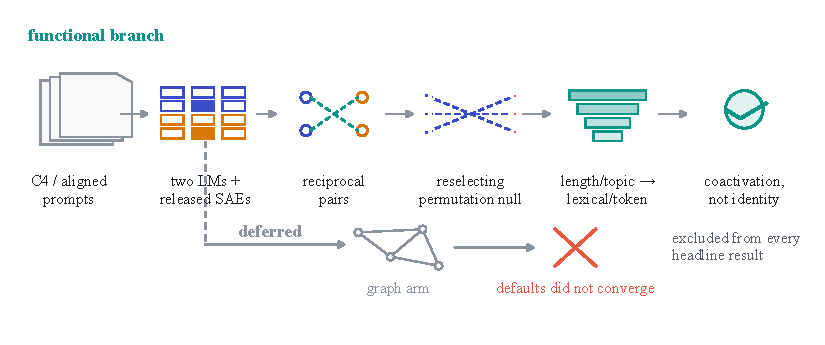
\includegraphics[width=1.0000\textwidth]{figures/integrated_20260923/fig02_redrawn.pdf}
\caption{\textbf{Functional evidence pipeline and its scope.} Shared text enters independently trained models and released SAEs; reciprocal pairs are tested with reselecting permutation nulls and a ladder of controls. The result concerns coactivation rather than feature identity. A deferred attribution-graph branch did not converge at the defaults and contributes no headline result. Icons and permutation links are schematic.}
\label{fig:pipeline}
\end{figure}

\section{Compute and scheduling}\label{app:scheduling}

Every headline (v1) result in this paper runs as a single-GPU job on one H100-80GB or
H200-141GB: the probe-attribution sweep is minutes per model (17 models, well under $10$
GPU-hours in total), and each cross-model SAE-matching cell --- the $2{,}000$-document C4
slice through both models plus the $200$-permutation null --- is under $1.5$ GPU-hours,
with the \texttt{.sbatch} scripts (in the code release) giving the exact allocation per cell.
Two appendix analyses, the filtered audit of \citet{lan2024universal} (\Cref{app:lan_filters}) and
the Gemma read-point sensitivity (\Cref{app:gemmahook}), ran wholly or partly on Apple MPS with ungated
Gemma-2 re-uploads, as stated there.

We do \emph{not} report a job DAG for the v0 attribution-graph pipeline: its graph-building
jobs never produced usable graphs (the influence propagation does not converge;
\Cref{app:deferred,app:v0_limitations}), so their requested allocations describe a plan, not
a reproducible cost behind any result here.

\section{Robustness}\label{app:robustness}

\paragraph{Pruning threshold sweep.} \emph{Not applicable to v1.}
The v1 probe-attribution scheme does not have a pruning threshold; the
threshold sweep was a robustness check for the v0 attribution-graph
backend, which is disclosed as non-convergent in \Cref{sec:disc:negative} and not
used for headline results.

\paragraph{Backend equivalence check.} \emph{Not applicable to v1.}
The v1 probe-attribution is implemented natively in
\texttt{transformers} + logit-lens hooks; no second backend is used.
Robustness across alternative attribution implementations is left
to follow-up work.

\section{Raw cross-lingual probe-attribution sweep}\label{app:probe_attribution}

Probe-attribution is a logit-lens-based, self-contained per-layer attribution scheme that
does \emph{not} require the \texttt{circuit\_tracer} library or attribution-graph
convergence. For each prompt and each layer $\ell$ we compute the logit-lens projection at
position $-1$ and define the per-layer attribution $a_\ell$ as the target-token logit under
this projection (the layer-$\ell$ residual passed through the model's final norm and
unembedding, read at the target token); we then compute the Pearson correlation $r$
between the per-layer attribution vectors for two languages $L_1,L_2$ on translated prompts,
restricted to mid-layers $\ell\in[L/4,3L/4)$. \Cref{tab:probe_attribution} reports the full
per-language-pair sweep. This metric does not directly verify circuit-level feature sharing;
\Cref{sec:results:construct-validity} shows it is largely a depth-profile artifact, so it is
reported here as the raw quantity that the construct-validity audit corrects, not as a
headline result.

\begin{table}[h]
\centering
\caption{\textbf{Cross-lingual mid-layer probe-attribution correlation, v2 ($n=20$ prompt-pairs per language).} Pairwise Pearson $r$ of per-layer logit-lens attribution between languages on aligned en/zh/ja/ko antonym prompts; mid-layer band $[L/4, 3L/4)$; bootstrap 95\% CI and permutation-test $p$ from $5{,}000$ shuffles in the per-model JSONs. Each model evaluated on an aligned $20$-pair multilingual probe set. Gemma3 shows substantially stronger and more scale-monotone alignment than Qwen3 on the identical prompt set --- which \Cref{sec:results:construct-validity} traces to the per-layer depth profile, not cross-lingual semantics.}
\label{tab:probe_attribution}
\small
\begin{tabular}{lrrrrr}
\toprule
Lang pair & Qwen3-0.6B & Qwen3-1.7B & Qwen3-4B & Qwen3-8B & Qwen3-14B \\
\midrule
en--zh & $+0.238$ & $+0.194$ & $+0.055$ & $+0.240$ & $-0.129$ \\
en--ja & $+0.122$ & $+0.222$ & $+0.057$ & $+0.218$ & $-0.191$ \\
en--ko & $+0.186$ & $+0.261$ & $-0.057$ & $+0.382$ & $+0.133$ \\
zh--ja & $+0.369$ & $+0.178$ & $+0.384$ & $+0.519$ & $+0.384$ \\
zh--ko & $+0.062$ & $+0.114$ & $+0.076$ & $+0.142$ & $+0.074$ \\
ja--ko & $+0.122$ & $+0.194$ & $+0.245$ & $+0.254$ & $-0.056$ \\
\midrule
\textbf{Mean} & $\mathbf{+0.183}$ & $\mathbf{+0.194}$ & $\mathbf{+0.127}$ & $\mathbf{+0.293}$ & $+0.036$ \\
\textbf{N pairs $r>0$} & 6/6 & 6/6 & 5/6 & 6/6 & 3/6 \\
\textbf{N pairs $p<0.01$} & 3/6 & 5/6 & 2/6 & 6/6 & 4/6 \\
\bottomrule
\end{tabular}

\medskip\noindent\textbf{Cross-family comparison (same $n=20$ prompt set).}\\[2pt]
\begin{tabular}{lrrr}
\toprule
Lang pair & Gemma3-4B-it & Gemma3-12B-it & Gemma3-27B-it \\
\midrule
en--zh & $+0.459$ & $+0.548$ & $+0.767$ \\
en--ja & $+0.601$ & $+0.689$ & $+0.781$ \\
en--ko & $+0.689$ & $+0.618$ & $+0.846$ \\
zh--ja & $+0.649$ & $+0.736$ & $+0.873$ \\
zh--ko & $+0.409$ & $+0.331$ & $+0.767$ \\
ja--ko & $+0.627$ & $+0.515$ & $+0.842$ \\
\midrule
\textbf{Mean} & $\mathbf{+0.572}$ & $\mathbf{+0.573}$ & $\mathbf{+0.813}$ \\
\textbf{N pairs $r>0$} & 6/6 & 6/6 & 6/6 \\
\textbf{N pairs $p<0.01$} & 6/6 & 6/6 & 6/6 \\
\bottomrule
\end{tabular}
\end{table}

\begin{table}[h]
\centering
\caption{\textbf{Construct-validity controls on the raw probe-attribution metric}
(mean over the six language pairs; verdict in \Cref{sec:results:construct-validity}).
\emph{real}: the headline metric, reproducing the
original v2 JSONs. \emph{residual} $=$ real $-$ mismatched. \emph{survival}
$=$ mismatched$/$real. ML $=$ multilingual. Layer-shuffle collapses every model to
$\approx 0$ while mismatched-pair survives $79$--$100\%$: the raw signal lives in the
depth profile, not in cross-lingual semantics.}
\label{tab:construct_validity}
\small
\begin{tabular}{llrrrrr}
\toprule
Model & ML & real $r$ & layer-shuffle (a) & mismatched (b) & residual & survival \\
\midrule
Pythia-1.4B  & no  & $+0.695$ & $+0.002$ & $+0.689$ & $+0.006$ & $99\%$ \\
Gemma3-4B    & yes & $+0.572$ & $+0.059$ & $+0.493$ & $+0.080$ & $86\%$ \\
Pythia-410M  & no  & $+0.553$ & $-0.005$ & $+0.553$ & $+0.000$ & $100\%$ \\
Gemma3-1B    & yes & $+0.336$ & $+0.059$ & $+0.279$ & $+0.057$ & $83\%$ \\
Qwen3-1.7B   & yes & $+0.194$ & $+0.040$ & $+0.153$ & $+0.041$ & $79\%$ \\
\midrule
\textbf{Mean} & & $\mathbf{+0.470}$ & $\mathbf{+0.031}$ & $\mathbf{+0.434}$ & $\mathbf{+0.037}$ & $\mathbf{89\%}$ \\
\bottomrule
\end{tabular}
\end{table}

\section{Power-law scaling of the raw metric}\label{app:scaling}

\emph{Caveat:} every number here is computed over the \emph{raw} probe-attribution metric,
which \Cref{sec:results:construct-validity} shows is largely a per-layer depth-profile
artifact. We retain the power-law analysis because it characterizes how that raw metric
behaves with scale; the ``architecture gates scale'' reading is a statement about the raw,
depth-confounded quantity, and the depth-corrected residual does \emph{not} support a
cross-lingual law (\Cref{sec:results:residual-scaleup}).

Fitting $r=c\,N^{b}$ (alignment $r$ vs.\ parameter count $N$) within each family, with
nonparametric bootstrap $95\%$ CIs over the within-family $(N,r)$ points ($10{,}000$ resamples;
\texttt{code/analysis/rosetta\_slope\_bootstrap.py}), the within-family scale slope is itself
architecture-dependent: Pythia shows a \emph{real} positive slope ($b=+0.43$, CI
$[+0.13,+0.80]$, $R^2=0.88$, $n=4$), Gemma3 a positive lower-bound-borderline one
($b=+0.24$, CI $[+0.00,+0.43]$, $R^2=0.90$, $n=4$), and Qwen3 \emph{none} ($b=-0.32$, CI
$[-1.25,+0.35]$). What is robust across all three families is that at matched parameter
count the family gap dwarfs the within-family scale effect: Pythia-$1.4$B ($r=0.70$) is
$3.6\times$ Qwen3-$1.7$B ($0.19$), the smallest Gemma3-$1$B ($0.34$) exceeds the best Qwen3
of any size (Qwen3-$8$B, $0.29$), and Gemma3-$4$B ($0.57$) is $16\times$ the Qwen3-$14$B
alignment ($0.04$). This is the measured form of ``architecture gates scale'' over the raw
metric --- a $3.6$--$16\times$ between-family gap dominating within-family slopes that range
from real (Pythia) to null (Qwen3); \Cref{fig:rosetta_sublinear}.

\begin{figure}[h]
\centering
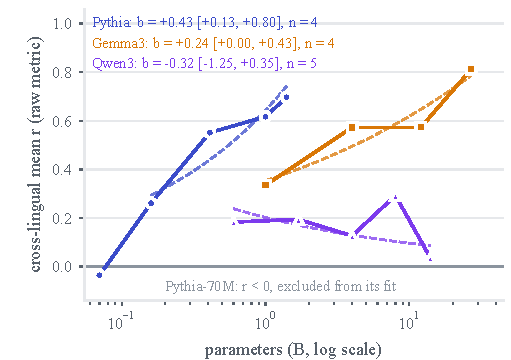
\includegraphics[width=0.62\textwidth]{figures/fig_rosetta_sublinear.pdf}
\caption{\textbf{Raw probe-attribution alignment vs.\ scale (depth-confounded; not a
cross-lingual result, \Cref{sec:results:secondary}).} Mean pairwise correlation $r$ vs.\ parameter count (log scale) for Pythia
($0.07$--$1.4$B), Qwen3 ($0.6$--$14$B), Gemma3 ($1$--$27$B), with power-law fits $r=c\,N^{b}$
(dashed); the key gives each family's exponent with its bootstrap $95\%$ CI
(\texttt{results/rosetta\_check/rosetta\_sublinear\_v0.json},
\texttt{rosetta\_slope\_bootstrap.json}). Pythia $b=+0.43$ (real; fit on the four positive-$r$
checkpoints, as the $70$M point has $r{<}0$ and is excluded from the log-log fit), Gemma3
$b=+0.24$, Qwen3 $b=-0.32$ (null). Computed over the \emph{raw}, depth-confounded metric.}
\label{fig:rosetta_sublinear}
\end{figure}

\section{Deferred attribution-graph analyses}\label{app:deferred}\label{sec:results:reproduce}\label{sec:results:negative}\label{sec:results:xlingual}\label{sec:results:thinking}\label{sec:results:scaling}

The v0 case-study reproduction targeted the qualitative case studies of
\citet{lindsey2025biology} (antonym, two-hop factual recall, and entity-recognition hallucination
prompts, reported on Claude 3.5 Haiku with the method of \citet{ameisen2025attribution}); our v0
\circuittracer{} setup (\Cref{app:failure_methods}) failed to converge on all four Qwen3 sizes (0.6B,
1.7B, 4B, 8B), producing zero valid \texttt{structure\_features} at default thresholds. Cross-lingual node-set Jaccard, thinking-mode dissection (\qwen{}'s
\texttt{enable\_thinking} toggle), and the attribution-graph $|V|\propto N^\beta$ power law
all depend on the same backend and are deferred for the same reason. The probe-attribution
sweep (\Cref{app:probe_attribution}) was run in its place; its raw metric tracks network depth
(\Cref{sec:results:secondary}), so it answers no cross-family scaling question.

\section{Ablation-based causal probes: full detail}\label{app:causal}

\paragraph{Finding 3 (causal probe): a single-feature ablation test is underpowered and does
not establish shared computation --- and its own null highlights the same discipline.} To
probe whether the reciprocal sharing reflects shared \emph{computation}, we ablate each
matched feature in each model (a forward hook subtracting its decoder contribution at the
SAE's layer; cf.\ the feature-level ablations of \citealp{marks2024sparse}) and correlate
the two per-prompt $\Delta$loss vectors over $150$ prompts
($30$ matched pairs), against a derangement null, for four pairs
(\texttt{results/cross\_model\_causal/}, \Cref{tab:causal}). The probe proves
\emph{underpowered}: individual SAE-feature ablation effects are small and sparse (stored signed mean $\Delta$loss
${\approx}5\times10^{-4}$--$6\times10^{-2}$ nats in magnitude), so per-prompt $\Delta$loss vectors are
near-degenerate and per-pair correlations pile up at exactly $\pm1$ --- $3/30$ pairs for the
within-family Gemma pair but $8$--$23/30$ for the cross-family pairs. The
permutation-on-the-mean statistic is therefore unreliable, and applying our own construct-validity
reflex catches it: Pythia-70M$\leftrightarrow$Mistral-7B shows a large nominal $z=28.3$
($p=0.001$) that is \emph{entirely} a degeneration artifact --- $23/30$ pairs are degenerate,
and dropping them turns the signal \emph{negative} (non-degenerate mean $-0.12$, $14\%$
positive). After the degeneration filter, only the within-family Gemma pair retains a weak
positive (non-degenerate mean $+0.13$, $63\%$ of pairs positive, permutation $p=0.038$), and
even it does not survive a conservative sign test ($p=0.36$); no cross-family pair shows a
clean positive.

We then \emph{upgraded the probe's power} as the degeneration analysis prescribes: ablate the
top-$30$ matched features \emph{jointly} in each model (a dense, large intervention ---
$\Delta$loss up to $+2$ nats, no $\pm1$ degeneration by construction) and test the correlation
of the two per-prompt $\Delta$loss vectors against a null of $200$ random same-size feature
groups from the same top-variance pool in model B
(\texttt{results/cross\_model\_causal\_group/}). The matched-group correlations \emph{look}
substantial (within-family Gemma $+0.48$; Gemma-9B$\leftrightarrow$Mistral $+0.59$), but the
random-group null reveals they are within chance variation: the null distribution is extremely
broad (SD $0.39$--$0.47$ for the two Gemma pairs, $95\%$ CI up to $+0.78$), because per-prompt group-ablation
$\Delta$loss is dominated by a \emph{generic prompt-fragility axis} --- almost any strong
ablation disrupts the same fragile prompts. No pair reaches significance
(within-family $p=0.25$; Gemma-9B$\leftrightarrow$Mistral $p=0.13$;
Pythia$\leftrightarrow$Mistral $p=0.30$), and critically the \emph{within-family positive
control fails}: a probe that cannot detect causal alignment where representational matching is
unambiguous ($z=17$ reciprocal sharing) cannot certify a cross-family null as a genuine
dissociation either. We therefore report cross-model coactivation at the
\emph{representational} level (Findings~1--2), not shared computation, and report that \emph{both} ablation-based
causal probes --- single-feature (degeneration) and multi-feature group (fragility-axis
confound) --- fail to resolve shared computation in either direction; within-model
activation-level steering transfer is reported below. The pattern is
this paper's thesis twice over: a nominal $z=28.3$ dissolves under a degeneration filter, and
a matched-group correlation of $+0.59$ dissolves under the right null --- the statistic, not
the phenomenon, can manufacture the effect.

The activation-level test we flagged as the key next step now exists: a
\emph{steering-transfer} probe that escapes both confounds above. For each of the $20$
interpretable matched pairs we steer each feature \emph{in its own model} ($h \mathrel{+}=
\beta\, s_f W_{\text{dec}}[f]$ at the SAE read point, $s_f$ the feature's natural activation
scale) and compare the \emph{identity} of the top-$30$ promoted tokens (decoded strings, so
tokenizer-robust; steering is a dense large intervention, so no degeneration; token identity
carries no prompt-fragility axis). Matched pairs share promoted-token strings far above a
$2000$-derangement null --- at $20$ pairs $0.70$ vs.\ $0.01$ expected ($z\approx41$--$44$,
$p=1/2001$, invariant across $\beta\in\{2,8\}$), and scaling to the top-$50$ mutual-NN
pairs at $\beta{=}2$ \emph{strengthens} it ($1.26$ vs.\ $0.01$, $z=94.2$, $56\%$ of pairs with $\geq$$1$
exact-string overlap) --- and it \emph{replicates on a second, independent pair}:
Qwen3-1.7B$\leftrightarrow$Gemma-2-2B gives $3.50$ vs.\ $0.05$ ($z=43.6$, $65\%$ of pairs
overlapping; the higher raw overlap is consistent with the larger Qwen/Gemma shared string
inventory). The token dumps are topically coherent --- the
cricket-matched pair promotes \emph{batsman/batting/cricket} in Gemma and
\emph{batt/caught/declared/conceded} in Mistral; the gambling pair
\emph{betting/blackjack/gambler} vs.\ \emph{ante/antes/dealt/ace}
(\texttt{results/cross\_model\_sae/steer*.json}). The raw number ($0.70$ of $30$) understates the effect because $30$ is the wrong
denominator: two empirical ceilings bound the statistic. Within-model self-agreement ---
the \emph{same} feature in the \emph{same} model at $\beta{=}2$ vs.\ $\beta{=}8$ ---
is only $6.8$--$9.3/30$, and the binding constraint is the \emph{shared promoted-string
inventory}: across all $20$ pairs only $16$ of Gemma's $453$ distinct promoted strings appear
anywhere in Mistral's promoted universe at all. Of those $16$ available strings, the
\emph{matched} feature captures $14$ ($88\%$), versus a $0.7\%$ capture rate under the
derangement null --- a ${\sim}125\times$ enrichment at this shared-inventory ceiling. We
therefore read the steering-transfer result as activation-level evidence consistent with
matched features playing similar functional roles (steering is within-model, not a
cross-model intervention), small in raw exact-string units for tokenizer reasons,
near-ceiling once the inventory bound is accounted for. On the Gemma side the injection site is
our read point, one block before the dictionary's training hook (\Cref{app:gemmahook}), so what
is measured there is the effect of adding the released decoder direction at that point.




\section{Full result tables}\label{app:tables}

Full tables, each summarized in the main text: the scaled residual controls
(\Cref{tab:residual_scaleup}), cross-model SAE feature matching on the templated corpus
(\Cref{tab:sae_matching}), the random-dictionary control (\Cref{tab:rand_control}), the C4
cells as raw counts (\Cref{tab:c4_counts}), the derangement null for the top-document audit
(\Cref{tab:interp_null}), the single-feature causal probe (\Cref{tab:causal}), and the
cross-lingual cells (\Cref{tab:xling_cells,fig:language_panel}). The C4 held-out confirmation is plotted in the
main text (\Cref{fig:heldout-main}), with exact values in \Cref{tab:c4_verdicts}; same-corpus discovery counts are in \Cref{tab:c4_counts}.

\begin{table}[h]
\centering
\caption{\textbf{SAE-matching roster and exact observational scope.} ``Read point'' is where we
apply the encoder; for every suite except Gemma Scope it is the dictionary's training hook.
Depth is hook layer over transformer blocks. $L_0$ is the release target or the mean nonzeros/token
(BOS included) measured at our read point by the tracked token-aligned extraction; ``n/r'' means
neither was encoded in the release ID nor retained in a tracked receipt, and is not inferred.
$^{\ddagger}$Gemma Scope dictionaries were trained on \texttt{resid\_post} of block $N$
(\texttt{hidden\_states[$N{+}1$]}) and we apply them to \texttt{hidden\_states[$N$]}, one block early
(\Cref{app:gemmahook}); without BOS their $L_0$ is ${\sim}75$ (2B) and ${\sim}48$ (9B) at our read point
and ${\sim}81$ and ${\sim}65$ at the training hook. Repository snapshot SHAs are in
\Cref{tab:model-revisions}. Every claim is conditional on these
(model, released SAE, read point, corpus, pooling) choices.}
\label{tab:sae-roster}
\scriptsize
\setlength{\tabcolsep}{2.5pt}
\resizebox{\textwidth}{!}{%
\begin{tabular}{lllllll}
\toprule
Model & release / repository & read point & depth & width & $L_0$ & recipe / provenance \\
\midrule
Gemma-2-2B & \texttt{gemma-scope-2b-pt-res-canonical} & \texttt{resid\_pre} block 12$^{\ddagger}$ & $12/26$ & 16k (65k check) & ${\sim}154$ & JumpReLU, Google Gemma Scope \\
Gemma-2-9B & \texttt{gemma-scope-9b-pt-res-canonical} & \texttt{resid\_pre} block 20$^{\ddagger}$ & $20/42$ & 16k & ${\sim}117$ & JumpReLU, Google Gemma Scope \\
Mistral-7B-v0.1 & \texttt{mistral-7b-res-wg} & \texttt{resid\_pre} block 16 & $16/32$ & 65,536 & ${\sim}88$ & SAE Lens; JoshEngels community release \\
Qwen3-1.7B-Base & \texttt{Qwen/SAE-Res-Qwen3-1.7B-Base-W32K-L0\_50} & \texttt{resid\_post} layer 14 & $14/28$ & 32,768 & 50 & TopK-ReLU, Qwen-Scope; manual audited loader \\
Qwen3-8B-Base & \texttt{Qwen/SAE-Res-Qwen3-8B-Base-W64K-L0\_50} & \texttt{resid\_post} layer 18 & $18/36$ & 65,536 & 50 & TopK-ReLU, Qwen-Scope; manual audited loader \\
Llama-3.2-1B & \texttt{chanind/sae-llama-3.2-1b-res} & \texttt{resid\_post} block 8 & $8/16$ & 16,384 & ${\sim}117$ & SAE Lens; chanind community release \\
\midrule
Pythia-70M (negative) & \texttt{pythia-70m-deduped-res-sm} & \texttt{resid\_post} block 3 & $3/6$ & 32,768 & n/r & SAE Lens release; registry lists no publication \\
GPT-2 (underpowered) & \texttt{gpt2-small-res-jb} & \texttt{resid\_pre} block 6 & $6/12$ & 24,576 & n/r & reformatted SAE Lens release \citep{bloom2024gpt2saes} \\
\bottomrule
\end{tabular}}
\end{table}


\begin{table}[h]
\centering
\caption{\textbf{Depth-corrected within-family residual at scale} ($n=206$ concept pairs,
$9$ families, en/zh/ja/ko; $17$ models). \emph{residual} $=$ real $-$ within-family
mismatched, the depth- and family-corrected cross-lingual component; $95\%$ CI from $10{,}000$
bootstrap resamples; \texttt{*} $=$ CI excludes $0$. EN $=$ English-only, ML $=$
multilingual. The residual is a \emph{real} per-model quantity ($10/17$ CIs exclude $0$)
but is \emph{not} cross-lingually specific: an English-only GPT-2 has the largest residual
of all $17$ models, the English-only mean exceeds the multilingual mean, and the
multilingual-vs-English-only gap is not significant by the model-level exact permutation
test ($p=0.79$).}
\label{tab:residual_scaleup}
\small
\begin{tabular}{lcrc@{\hspace{1.5em}}lcrc}
\toprule
Model & type & residual & sig & Model & type & residual & sig \\
\midrule
GPT-2          & EN & $+0.204$ & * & Qwen3-8B      & ML & $+0.063$ & * \\
Qwen3-0.6B     & ML & $+0.166$ & * & BLOOM-560M    & ML & $+0.050$ & * \\
Qwen3-4B       & ML & $+0.149$ & * & Qwen3-1.7B    & ML & $+0.023$ & * \\
GPT-2-medium   & EN & $+0.139$ & * & Gemma3-4B     & ML & $+0.022$ & * \\
GPT-Neo-125M   & EN & $+0.109$ & * & Gemma3-1B     & ML & $+0.010$ & \\
OPT-125M       & EN & $+0.104$ & * & Gemma2-2B     & ML & $+0.010$ & \\
               &    &          &   & Qwen2.5-0.5B  & ML & $+0.010$ & \\
               &    &          &   & Pythia-1.4B   & EN & $-0.001$ & \\
               &    &          &   & Pythia-1B     & EN & $-0.006$ & \\
               &    &          &   & Pythia-410M   & EN & $-0.006$ & \\
               &    &          &   & Gemma3-12B    & ML & $-0.006$ & \\
\bottomrule
\end{tabular}

\medskip
\begin{tabular}{lr}
\toprule
English-only mean (7 models) & $+0.078$ \\
Multilingual mean (10 models) & $+0.050$ \\
Gap (multilingual $-$ English-only) & $-0.028$ \quad CI $[-0.052,-0.004]$ \\
Model-level exact permutation $p$ (gap $\geq$ obs; $19{,}448$ = \emph{17 choose 7}) & $0.79$ \\
Model-level exact permutation $p$, two-sided & $0.42$ \\
Pair-level permutation $p$, one-sided ($206{\times}6$ concept pairs per model) & $0.499$ \\
Pair-level permutation $p$, two-sided & $0.98$ \\
Significant-positive split & $4/7$ EN, $6/10$ ML \\
\bottomrule
\end{tabular}
\end{table}

\begin{table}[!htp]
\centering
\caption{\textbf{Cross-model SAE feature matching} ($206$ English prompts, top-$1{,}500$
features, $200$-permutation null). \emph{greedy exc.}: greedy-max mean correlation minus its
null. \emph{Hung.}: optimal one-to-one matched correlation. \emph{mutual-NN $z$}: count of
reciprocal best-buddy feature pairs as a $z$-score over the permutation null,
$(\text{count}-\text{null mean})/\text{null SD}$. Pairs measured at multiple depth bands show
the range. \emph{within} $=$ same family (Gemma-2, three depth bands);
\emph{cross-modern} $=$ different families (Gemma-2 / Mistral-7B / Pythia, $70$M--$9$B);
\emph{cross-GPT2} $=$ a pair including the older GPT-2. The strict mutual-NN $z$ is the
construct-valid measure; greedy and Hungarian are shown to be confounded.}
\label{tab:sae_matching}
\small
\setlength{\tabcolsep}{4pt}
\resizebox{\textwidth}{!}{%
\begin{tabular}{llrrr}
\toprule
Model pair (depth bands) & class & greedy exc. & Hung. & mutual-NN $z$ \\
\midrule
Gemma2-2B $\leftrightarrow$ Gemma2-9B \ {\footnotesize(early/mid/late)} & within & $+0.77$--$0.79$ & $0.75$--$0.89$ & $15.4$--$21.9$ \\
\midrule
Pythia-70M $\leftrightarrow$ Mistral-7B        & cross-modern & $+0.36$ & $0.70$ & $21.9$ \\
Gemma2-9B $\leftrightarrow$ Mistral-7B \ {\footnotesize(early/mid/late)} & cross-modern & $+0.67$--$0.72$ & $0.32$--$0.46$ & $13.9$--$16.7$ \\
Gemma2-2B $\leftrightarrow$ Mistral-7B \ {\footnotesize(early/mid/late)} & cross-modern & $+0.74$--$0.75$ & $0.18$--$0.26$ & $6.9$--$10.8$ \\
Pythia-70M $\leftrightarrow$ Gemma2-9B         & cross-modern & $+0.36$ & $0.32$ & $4.6$ \\
\midrule
Gemma2-2B $\leftrightarrow$ GPT-2              & cross-GPT2 & $+0.81$ & $0.82$ & $4.2$ \\
Gemma2-9B $\leftrightarrow$ GPT-2              & cross-GPT2 & $+0.69$ & $0.69$ & $0.5$ \\
GPT-2 $\leftrightarrow$ Mistral-7B             & cross-GPT2 & $+0.79$ & $0.00$ & $-1.3$ \\
Pythia-70M $\leftrightarrow$ GPT-2             & cross-GPT2 & $+0.03$ & $0.02$ & $-1.2$ \\
\bottomrule
\end{tabular}}
\\[3pt]
{\footnotesize Every cross-modern $z$ has $p=1/201$ at \emph{every} depth band; all
cross-GPT2 pairs except Gemma2-2B$\leftrightarrow$GPT-2 are n.s.\ ($p\geq0.37$). Observed
mutual-NN counts are $1.2$--$2.4\times$ their nulls. Full per-pair counts/nulls/$p$ in
\texttt{results/cross\_model\_sae/SUMMARY.json}.}
\end{table}

\begin{table}[h]
\centering
\caption{\textbf{Random-dictionary control: both the observation and its null move}
(three representative C4-robust cells; same
corpus, pooling, and permutation null as \Cref{tab:c4_verdicts}, with each side's trained
SAE dictionary replaced by random unit directions of the same $d_{\text{sae}}$, top-$k$
sparsified with $k$ calibrated to that SAE's mean $L_0$, independent seeds per side).
Reciprocal counts collapse while the permutation null \emph{rises}, so the negative
mutual-NN $z$ is not an effect size; the greedy statistic moves the other way, rising under
random dictionaries --- an independent confirmation of Finding~2. Discussion:
\Cref{sec:results:sae-matching}. Receipts: \texttt{rand\_c4\_*.json}.}
\label{tab:rand_control}
\footnotesize
\setlength{\tabcolsep}{4pt}
\begin{tabular}{lrrrrrr}
\toprule
& \multicolumn{3}{c}{trained SAE} & \multicolumn{3}{c}{random dictionary} \\
\cmidrule(lr){2-4}\cmidrule(lr){5-7}
Cell & obs & null $\mu$ & mutual $z$ / greedy $z$ & obs & null $\mu$ & mutual $z$ / greedy $z$ \\
\midrule
Qwen3-1.7B $\leftrightarrow$ Gemma2-2B & $811$ & $371.8$ & $+42.7$ / $+180.7$ & $152$ & $604.7$ & $-29.0$ / $+370.2$ \\
Gemma2-9B $\leftrightarrow$ Mistral-7B & $819$ & $553.4$ & $+24.0$ / $+84.6$ & $212$ & $607.0$ & $-26.8$ / $+241.9$ \\
Llama-3.2-1B $\leftrightarrow$ Mistral-7B & $551$ & $434.9$ & $+12.3$ / $+19.1$ & $223$ & $584.5$ & $-24.1$ / $+123.6$ \\
\bottomrule
\end{tabular}
\end{table}

\begin{table}[h]
\centering
\caption{\textbf{C4 same-corpus discovery cells as effect sizes, not only $z$} (the screen preceding
\Cref{tab:c4_verdicts}: $2{,}000$ C4 documents, top-$1{,}500$ mutual-NN features, $200$-permutation
null). \emph{obs}: reciprocal best-buddy count; \emph{null $\mu{\pm}\sigma$}: permutation mean and SD;
\emph{excess}: $(\text{obs}-\mu)$ as a fraction of the $1{,}500$-feature pool --- the practical
effect size the $z$ standardizes. The excess ranges from ${\sim}30\%$ of the pool (within-family)
to $8$--$10\%$ (the weakest survivors, Qwen3-1.7B and Llama-3.2-1B) and is \emph{negative} for the
Pythia failure. The recipe-check row is the same model pair as the Gemma2-2B row with only
the released Gemma dictionary width swapped $16$k$\to$$65$k; it moves the cell by
$-6.3$ excess points and $-8.0$ in $z$ with no change of model, which is why we do not read
the ordering of $z$ across cells as a capability trend
(\Cref{sec:results:sae-matching}). Per-cell receipts: \texttt{results/cross\_model\_sae/c4\_*.json}.}
\label{tab:c4_counts}
\footnotesize
\setlength{\tabcolsep}{4pt}
\begin{tabular}{llrrrr}
\toprule
Cell & class & obs & null $\mu{\pm}\sigma$ & excess & $z$ \\
\midrule
Gemma2-2B $\leftrightarrow$ Gemma2-9B & within & $882$ & $430.8{\pm}10.1$ & $+30.1\%$ & $44.7$ \\
Qwen3-8B $\leftrightarrow$ Qwen3-1.7B & within & $842$ & $408.5{\pm}11.4$ & $+28.9\%$ & $38.2$ \\
\midrule
Qwen3-1.7B $\leftrightarrow$ Gemma2-2B & cross-family & $811$ & $371.8{\pm}10.3$ & $+29.3\%$ & $42.7$ \\
Qwen3-8B $\leftrightarrow$ Gemma2-9B & cross-family & $859$ & $471.8{\pm}10.4$ & $+25.8\%$ & $37.1$ \\
Qwen3-8B $\leftrightarrow$ Gemma2-2B & cross-family & $784$ & $402.7{\pm}9.6$ & $+25.4\%$ & $39.8$ \\
Qwen3-1.7B $\leftrightarrow$ Gemma2-9B & cross-family & $774$ & $434.6{\pm}9.9$ & $+22.6\%$ & $34.2$ \\
Gemma2-9B $\leftrightarrow$ Mistral-7B & cross-family & $819$ & $553.4{\pm}11.1$ & $+17.7\%$ & $24.0$ \\
Qwen3-8B $\leftrightarrow$ Mistral-7B & cross-family & $777$ & $515.4{\pm}10.0$ & $+17.4\%$ & $26.2$ \\
Gemma2-2B $\leftrightarrow$ Mistral-7B & cross-family & $688$ & $469.7{\pm}9.9$ & $+14.6\%$ & $22.1$ \\
Qwen3-1.7B $\leftrightarrow$ Mistral-7B & cross-family & $620$ & $475.0{\pm}11.6$ & $+9.7\%$ & $12.5$ \\
Llama-3.2-1B $\leftrightarrow$ Mistral-7B & cross-family & $551$ & $434.9{\pm}9.4$ & $+7.7\%$ & $12.3$ \\
\midrule
Gemma2-2B(w$65$k) $\leftrightarrow$ Mistral-7B & recipe check & $473$ & $348.1{\pm}8.9$ & $+8.3\%$ & $14.1$ \\
Pythia-70M $\leftrightarrow$ Mistral-7B & cross-scale & $390$ & $411.1{\pm}10.9$ & $-1.4\%$ & $-1.9$ \\
\bottomrule
\end{tabular}
\end{table}

\begin{table}[h]
\centering
\caption{\textbf{Derangement null for the top-document audit.} The ``auditable by reading''
statistic is the mean size of the intersection of the two sides' top-$5$ max-activating C4
documents, over the $k$ mutual-NN matched pairs. Null: hold both sides' document sets fixed
and re-pair them under $2{,}000$ random derangements (no feature keeps its partner) --- the
question ``would \emph{any} pairing of these topical features share documents?''. \emph{max
doc share}: largest fraction of all top-doc slots taken by a single document (a
document-popularity artifact would drive this up). Every cell floors the empirical $p$ at
$1/(2000{+}1)$. Slots whose activation is exactly $0$ are excluded: SAE activations are
sparse and \texttt{argsort} breaks ties by index, so two models can select the same
arbitrary zero-activation documents and manufacture overlap. This is real but tiny here
($8$ zero slots in $1{,}100$, all in the held-out arm, contributing one overlap count;
the held-out mean moves $2.35\to2.30$). The top-$5$ endpoint is a convention and is not
load-bearing: recomputing at top-$3$ leaves every cell at the $p$ floor
($z=43$--$136$). Receipt:
\texttt{results/cross\_model\_sae/INTERP\_OVERLAP\_NULL.json}
(\texttt{code/analysis/interp\_overlap\_null.py}).}
\label{tab:interp_null}
\footnotesize
\setlength{\tabcolsep}{3.5pt}
\begin{tabular}{llrrrrrr}
\toprule
Cell & corpus & $k$ & obs & null $\mu{\pm}\sigma$ & null max & $z$ & max doc share \\
\midrule
Gemma2-9B $\leftrightarrow$ Mistral-7B & C4 in-sample & $20$ & $3.35$ & $0.031{\pm}0.040$ & $0.25$ & $82.2$ & $2\%$ \\
Gemma2-9B $\leftrightarrow$ Mistral-7B & C4 in-sample & $50$ & $3.40$ & $0.020{\pm}0.025$ & $0.16$ & $137.3$ & $1\%$ \\
Gemma2-9B $\leftrightarrow$ Mistral-7B & held-out half & $20$ & $2.30$ & $0.035{\pm}0.044$ & $0.30$ & $51.1$ & $2\%$ \\
Qwen3-1.7B $\leftrightarrow$ Gemma2-2B & C4 in-sample & $20$ & $3.60$ & $0.041{\pm}0.044$ & $0.25$ & $81.6$ & $3\%$ \\
\bottomrule
\end{tabular}
\end{table}

\paragraph{In one cell, the overlap is not a document-length or coarse-topic covariate.}\label{app:lencov} One worry is that the ``shared'' features are an artifact of the probe documents' surface covariates rather than shared representation. We re-run one cross-family cell (Gemma2-2B$\leftrightarrow$Mistral-7B, $+14.6\%$ excess --- seventh of the nine cross-family cells by excess, not the strongest, which is Qwen3-1.7B$\leftrightarrow$Gemma2-2B at $+29.3\%$) under two covariate-\emph{matched} permutation nulls that reproduce a covariate inside the null itself: permuting the second model's documents only within document-length deciles, and only within TF-IDF topic clusters ($k{=}10$). The excess is essentially unmoved --- $+14.6\%$ (random) $\to$ $+14.3\%$ (length-matched, $z{=}19.3$) $\to$ $+14.6\%$ (topic-matched, $z{=}20.5$), all $p{=}1/201$ --- so document length explains only ${\sim}2.5\%$ of the excess and coarse topic overlap ${\sim}0\%$: in this cell the overlap is not a length- or coarse-topic-covariate artifact (baseline reproduces the Table~\ref{tab:c4_counts} cell to $\pm1$ pair). One honest qualification: word-\emph{order} scrambling of the documents does \emph{not} shrink the excess ($+16.1\%$), which is expected rather than reassuring --- the C4 statistic mean-pools SAE activations over token positions, so it largely discards word order and a token scramble is a weak destructive probe for \emph{this} metric (weak, not null --- the pooled per-token activations remain context-dependent, so the excess shifts slightly under scrambling rather than staying fixed). At this stage the surviving overlap could still be lexical/token-level shared structure (it is robust to document length and coarse topic, and not attenuated by word-order scrambling); the lexical residualization and token-aligned tests below address that alternative. It is not evidence of shared compositional or syntactic features. Lexical composition is \emph{itself} a shared-document covariate, and the two matched nulls above do not remove it. Receipt: \texttt{results/cross\_model\_sae/covctl\_c4\_gemma2-2b\_\_mistral7b.json}.

\paragraph{Length and coarse-topic nulls and random splits on all nine cells (after submission).}\label{app:ninecell}
Registered before any output (\texttt{notes/PREREG\_ninecell\_ladder\_20260926.md}; decision rule: a
cell survives a control if $p\le0.05/18$ and $R\ge0.5$). The submitted version reported this design on
five cells, from pooled features extracted separately for \Cref{app:gemmahook} on a local machine (Apple
MPS, ungated Gemma-2 re-uploads), under a registered deviation committed while the cluster was
unreachable. The registered run itself finished on the cluster after the submission deadline. It
extracts features for all nine cells with the published pipeline and the original weights, and
\Cref{tab:ninecell} now reports it. In every cell it reproduces the published screen count to within
two pairs and the consecutive-split held-out excess to within $0.003$ (registered reproduction gate:
$\pm3$ pairs, $\pm0.005$). Each null is calibrated, as in \eqref{eq:ratio}, against $20$ partitions
with the same block sizes and random membership. Length deciles leave $R_{\text{len}}=0.968$--$1.003$
and coarse topic ($k{=}10$) leaves $R_{\text{top}}=0.986$--$0.997$, every arm at $p=1/2001$ (registered
branch A1). This includes the three Qwen3-8B cells, which had neither null in the submitted version
($R_{\text{len}}=0.988$--$0.992$, $R_{\text{top}}=0.994$--$0.997$). Ten seeded random $50/50$ splits of
the $2{,}000$ documents per cell replace the consecutive halves: all $90$ held-out tests give
$p=1/2001$ (branch B1). The median held-out excess over the ten splits is $0.972$--$1.006$ times that
of the consecutive split ($\rho$ in \Cref{tab:ninecell}), so the median is within $3\%$ of the
consecutive split; single splits differ by up to $6.4\%$ (Gemma-2-2B$\leftrightarrow$Mistral-7B, $0.530$
vs.\ $0.566$), and the smallest single-split held-out excess is $0.494$. On the five cells that both runs
cover, the two agree to within $0.002$ in $R_{\text{len}}$, $0.007$ in $R_{\text{top}}$ and $0.003$ in
$\Delta_E$.

\emph{Withdrawn after submission: the bootstrap intervals and the C1 reading.} The registration also
specified a bootstrap over evaluation documents (with replacement, pairs frozen) for $\Delta_E$ and for
each $R$. The submitted version printed its $95\%$ percentile intervals for $\Delta_E$ and read the
registered interval branch as C1. We withdraw both. A diagnosis registered after submission
(\texttt{notes/PREREG\_F1\_bootstrap\_diagnosis\_20261004.md}; receipt
\texttt{results/f1\_bootstrap\_diag\_20261004/}) recomputed every interval from the stored draws (the
percentile arithmetic is exact) and found three faults. (i)~Resampling does not reproduce the statistic
it resamples: across resamples the mean unrestricted excess is $1.05$--$1.46$ times the observed one.
(ii)~For $R_{\text{len}}$ and $R_{\text{top}}$, the permutation noise inside each resample ($100$
permutations, five calibration partitions) is $0.56$--$1.48$ times the bootstrap SD, so these intervals
largely measure Monte Carlo noise. (iii)~On planted data with a known value, the same $\Delta_E$
procedure covers the truth in $94.5\%$ of Gaussian datasets but in only $65\%$ and $70.5\%$ of sparse,
heavy-tailed ones ($200$ datasets each). On the cluster run the $\Delta_E$ bootstrap medians sit
$1.2$--$2.8$ SD below the point estimate, and $15$ of the $42$ intervals exclude their own point
estimate. The registered interval rule presupposes valid intervals, so the registered reading is C0
(instrument failed) and no interval is reported. No verdict rested on these intervals; variability is
shown by the $90$ random splits above.

Separately, the fine-topic receipts of the three ladder cells (\Cref{tab:covctl}), computed on the
main-table features, carry an uncalibrated length-decile arm, not reported before, that leaves
$1.002$, $0.993$ and $0.964$ of the excess (Qwen3-1.7B$\leftrightarrow$Gemma-2-2B,
Gemma-2-9B$\leftrightarrow$Mistral-7B, Llama-3.2-1B$\leftrightarrow$Mistral-7B; each $p=1/2001$,
$n_{\text{perm}}{=}2{,}000$). In the submitted version, with the Gemma-2-2B$\leftrightarrow$Mistral-7B
null above, six of the nine cells had a length-decile null and five a coarse-topic null; the cluster
run covers all nine. The fine-topic, lexical and token rungs still cover only the three ladder cells,
and they are point estimates. Receipts: \texttt{results/ninecell\_20260926/} (cluster run; the
submitted five-cell run is in \texttt{local\_mps\_cache/}).

\begin{table}[h]
\centering
\caption{\textbf{Length and coarse-topic nulls and random splits on all nine cells: registered run,
after submission} (original weights, published feature pipeline; \Cref{app:ninecell}). $R$: retention
against $20$ size-matched random partitions, $n_{\text{perm}}{=}2{,}000$, every $p=1/2001$. $\Delta_E$:
consecutive-split held-out excess; no interval is reported (the registered document bootstrap is
withdrawn, \Cref{app:ninecell}). Random split: range of held-out $\Delta_E$ over ten seeded $50/50$
splits (all $p=1/2001$); $\rho$: median of those ten over the consecutive $\Delta_E$; median $r$ over
the same splits. Q/G/M/L $=$ Qwen3/Gemma-2/Mistral/Llama-3.2, number $=$ size (B). Generated by
\texttt{code/analysis/emit\_ninecell\_table.py} from \texttt{results/ninecell\_20260926/}.}\label{tab:ninecell}
\footnotesize
% AUTO-GENERATED by code/analysis/emit_ninecell_table.py -- DO NOT HAND-EDIT.
% Source: results/ninecell_20260926/cluster_18577359/{A,B}_<cell>.json (cluster run, after
% submission); no bootstrap interval is printed (withdrawn, results/f1_bootstrap_diag_20261004/).
\begin{tabular}{@{}lrrrrrrr@{}}
\toprule
Cell & $M$ & $R_{\text{len}}$ & $R_{\text{top}}$ ($k{=}10$) & $\Delta_E$ & random split $\Delta_E$ & $\rho$ & median $r$ \\
\midrule
Q1.7--G2 & $811$ & $1.003$ & $0.994$ & $0.732$ & $0.714$--$0.740$ & $0.992$ & $0.933$ \\
Q1.7--G9 & $775$ & $0.987$ & $0.996$ & $0.677$ & $0.661$--$0.687$ & $0.994$ & $0.884$ \\
Q1.7--M & $621$ & $0.973$ & $0.986$ & $0.527$ & $0.494$--$0.535$ & $0.979$ & $0.734$ \\
Q8--G2 & $785$ & $0.992$ & $0.997$ & $0.698$ & $0.677$--$0.695$ & $0.983$ & $0.894$ \\
Q8--G9 & $860$ & $0.988$ & $0.994$ & $0.681$ & $0.672$--$0.689$ & $0.999$ & $0.863$ \\
Q8--M & $774$ & $0.988$ & $0.994$ & $0.601$ & $0.580$--$0.599$ & $0.981$ & $0.775$ \\
G2--M & $690$ & $0.974$ & $0.996$ & $0.566$ & $0.530$--$0.565$ & $0.972$ & $0.790$ \\
G9--M & $819$ & $0.994$ & $0.994$ & $0.603$ & $0.597$--$0.619$ & $1.004$ & $0.791$ \\
L1--M & $551$ & $0.968$ & $0.995$ & $0.518$ & $0.513$--$0.533$ & $1.006$ & $0.734$ \\
\bottomrule
\end{tabular}

\end{table}

\begin{table}[h]
\centering
\caption{\textbf{Fine-grained lexical/topic-matched null.} Mutual-NN excess (observed $-$ null mean) on three representative C4-robust cells under a permutation restricted to $k$-way TF-IDF/KMeans topic strata, $n_{\text{perm}}{=}2{,}000$. \emph{base}: unrestricted null. \emph{bow}: topic-matched. \emph{size-rnd}: strata with the \emph{same block sizes} but random membership, so they carry no lexical information --- this calibrates the mechanical shrinkage that any fine partition induces (permuting inside small blocks approaches the identity; at block size $1$ the excess is $0$ by construction). $R=\text{bow}/\text{size-rnd}$ is therefore the \emph{lexical-specific} retention; the raw bow$/$base ratio is shown for completeness but is confounded by that shrinkage. Receipts: \texttt{covctl\_k*\_c4\_*.json}.}
\label{tab:covctl}
\footnotesize
\setlength{\tabcolsep}{4pt}
\begin{tabular}{llrrrrrr}
\toprule
Cell & band & $k$ & blk & base & bow & size-rnd & $R$ \\
\midrule
Qwen3-1.7B $\leftrightarrow$ Gemma2-2B & strong & $200$ & $10$ & $+438.8$ & $+379.2$ & $+407.6$ & $0.930$ \\
Qwen3-1.7B $\leftrightarrow$ Gemma2-2B & strong & $500$ & $4$ & $+438.8$ & $+243.8$ & $+247.9$ & $0.983$ \\
\midrule
Gemma2-9B $\leftrightarrow$ Mistral-7B & median & $200$ & $10$ & $+267.5$ & $+257.0$ & $+260.7$ & $0.986$ \\
Gemma2-9B $\leftrightarrow$ Mistral-7B & median & $500$ & $4$ & $+267.5$ & $+217.9$ & $+205.5$ & $1.060$ \\
\midrule
Llama-3.2-1B $\leftrightarrow$ Mistral-7B & weak & $200$ & $10$ & $+112.7$ & $+108.8$ & $+109.3$ & $0.996$ \\
Llama-3.2-1B $\leftrightarrow$ Mistral-7B & weak & $500$ & $4$ & $+112.7$ & $+81.0$ & $+80.1$ & $1.012$ \\
\bottomrule
\end{tabular}
\end{table}


\paragraph{The topic-matched null at fine granularity, with its own confound removed.}
Ten clusters over $2{,}000$ documents is coarse, and one may ask whether
narrower topical structure would explain the sharing. We therefore re-ran the matched null
at $k{=}200$ and $k{=}500$ TF-IDF/KMeans clusters, at $n_{\text{perm}}{=}2{,}000$, on three
representative C4-robust cells --- the strongest, a median, and the weakest surviving
cross-family pair (\Cref{tab:covctl}).

Reading this requires a correction that is easy to miss, and that we got wrong in our own
first design. Permuting \emph{within} strata approaches the identity as the strata shrink:
at $k{=}200$ the mean block is $10$ documents and at $k{=}500$ it is $4$, so the null mean
rises toward the observed count and the excess decays for a reason having nothing to do with
topic --- at block size $1$ the excess is exactly $0$ by construction. The mean hides the shape at
$k{=}500$: on this slice KMeans returns one cluster of $1{,}490$ documents, $493$ single documents and
six small blocks (block sizes are stored in the receipts of \Cref{app:ninecell}), so the $k{=}500$ arm
holds about a quarter of the documents in place and permutes the rest. The size-matched arm has the
same block sizes, so $R$ is still a valid ratio, but $k{=}500$ is not a finer topic control than
$k{=}200$. The raw
bow$/$base ratio duly falls, to $0.56$ for the strongest cell at $k{=}500$, which read
naively would look like substantial topic-driven sharing. It is not. Permuting within strata
that have the \emph{same block-size multiset} but random membership --- carrying no lexical
information whatever --- removes essentially the same amount ($+247.9$ vs.\ $+243.8$ for
that cell). The lexical-specific retention $R$ (bow over size-matched-random) is
$0.93$--$1.06$ across all six cell$\times k$ results, with every topic-matched $p$ at the
$1/2001$ floor: \emph{the topic partition leaves at least $93\%$ of the excess that a
size-matched random partition leaves}. These six values use one random calibration partition; with
the calibration averaged over $20$ partitions (registered run, after submission; \Cref{tab:ladder})
they are $0.927$--$1.033$, and one partition alone moves the $k{=}500$ median cell between $1.006$ and
$1.101$. The decision rule and its thresholds were registered in the
repository before any of these receipts existed.

Three limits bound what this shows, and we state them because the control is easy to
over-read. \emph{(i)} The size-matched arm fixes the block-size \emph{distribution} but not
which documents land in large blocks --- KMeans puts generic documents in big clusters while
the random version scatters them --- so the calibration is first-order, not exact.
\emph{(ii)} TF-IDF/KMeans is itself a bounded lexical model: surviving it excludes shared
\emph{topic} detectors at $200$--$500$-way granularity, not lexical structure that clustering
does not represent. \emph{(iii)} The statistic is still mean-pooled and order-insensitive, so
shared \emph{token-level} detectors remain a live alternative (\Cref{sec:limitations}); this
control does not touch that hypothesis. What it does remove is the specific and most-cited
alternative --- that the surviving cells are two models' topic detectors co-firing on the
same documents. One incidental benefit: because these runs use $n_{\text{perm}}{=}2{,}000$,
their plus-one floor of $1/2001$ clears Bonferroni over the full C4 roster
($0.05/13=0.0038$, and $0.05/17=0.0029$ counting the GPT-2 cells), which the primary
$n_{\text{perm}}{=}200$ runs do not.

\paragraph{The lexical-residualization test, at a corpus size where it is interpretable.}\label{app:lexres} The natural control is to residualize each feature's per-document activation against a lexical representation before matching. Our first attempt (receipt \texttt{lexres\_c4\_gemma2-2b\_\_mistral7b.json}: TF-IDF$\to$SVD at $k\in\{64,128,256\}$, $2{,}000$ documents, $5$-fold cross-fitted OLS) returned an excess surviving at every $k$ --- and we did not report that as survival, because a \emph{random} subspace of identical rank removed just as much (${\sim}99\%$ retained; the ${\sim}5$-pair gap sits inside the null SD of ${\approx}11$). Nothing had been removed: the first stage explained a median $3.7\%$ and $1.3\%$ of feature variance out-of-fold, the SVD arms weaker still. An intervention that removes no more variance than a random subspace of equal rank cannot exclude anything.

That inadequacy was itself the finding, and it prescribed the fix: a pre-registered first-stage adequacy gate, and tracking whether the \emph{original} pairs disappear rather than whether a similar total is recomputed from different pairs. Both are now implemented (\texttt{code/analysis/lexical\_token\_test.py}, design pre-registered before the code was written), at $20{,}000$ documents rather than $2{,}000$. At that size the first stage is no longer inert: it beats a spectrum-matched \emph{shuffled} design at every $k$, with $99$--$100\%$ of features improving and median $\Delta R^2$ rising to $+0.31$ at $k{=}4096$ --- the gate the earlier run would have failed. \emph{What that $\Delta R^2$ is, exactly.} The registered adequacy rule is \texttt{frac}$(R^2_{\text{real}}>R^2_{\text{shuf}})\ge0.75$ \emph{and} median$(R^2_{\text{real}})-$median$(R^2_{\text{shuf}})\ge0.02$: it requires the real design to beat the shuffled one, and never requires $R^2_{\text{real}}>0$. Since the shuffled design predicts badly, and worse as $k$ grows (median $R^2_{\text{shuf}}\approx-0.013$ at $k{=}256$, $-0.048$ at $1024$, $-0.172$ at $4096$), $\Delta R^2$ overstates the fit by roughly that offset. The real design's own median out-of-fold $R^2$ at $k{=}4096$ is $0.129/0.140$, $0.101/0.036$ and $0.028/0.036$ for the strong, median and weak cells (\Cref{tab:lextok}) --- and on the Mistral side it is \emph{lower} at $k{=}4096$ ($0.036$) than at $k{=}256$ ($0.042$), so the entire rise in $\Delta R^2$ with $k$ on that side is the shuffled arm degrading, not the nuisance model getting stronger. The comparison against the earlier $2{,}000$-document run ($0.037$/$0.013$, at $k\le256$) is therefore only meaningful at matched rank: at $k{=}256$ on $20{,}000$ documents the per-side medians are $0.042$--$0.112$. Note also that these are medians over features, so ``$R^2$ of $0.14$'' bounds the typical feature, not every feature. The mutual-NN pairs are frozen on the raw features, and the test asks whether \emph{those} pairs still co-activate. They do, in all three cells and across all three strength bands: $R_{\text{lex}}=0.93$ (Qwen3-1.7B$\leftrightarrow$Gemma2-2B, strong, $822$ pairs), $0.94$ (Gemma2-9B$\leftrightarrow$Mistral-7B, median, $806$) and $0.92$ (Llama-3.2-1B$\leftrightarrow$Mistral-7B, weak, $520$) at the governing $k$, $p$ at the $1/2001$ floor (\Cref{tab:lextok}); retention against the shuffled design is $1.000$ exactly, so the residualization is removing real lexical structure rather than capacity.

Three limits, stated rather than buried. The statistic remains order-insensitive, so this bounds shared \emph{lexical} structure at the ranks tested rather than excluding token-level detectors outright --- the shared-unigram hypothesis is narrowed, not closed. The nuisance design is itself restricted, and the scope of ``removing the lexical signal'' is exactly that design and no wider: stopword-stripped \emph{unigram} TF-IDF over at most $50{,}000$ terms (\texttt{TfidfVectorizer(max\_features=50000, stop\_words="english")}, default \texttt{ngram\_range=(1,1)}), reduced by truncated SVD to $k\le4096$ components that retain $67.7\%$ of even that restricted design's variance. Nothing here bounds bigram or higher-order lexical structure, positional or stopword-carried structure, or the $32.3\%$ of the unigram design's own variance that the truncation discards. And the frozen pair counts differ sharply between cells ($822$/$806$/$520$), so the weak Llama--Mistral cell's retention is the noisiest measurement of the three; we flagged that before the numbers existed rather than after.

\begin{table}[h]
\centering
\caption{\textbf{Does the sharing survive residualizing on a unigram lexical model?} $20{,}000$ C4 documents, $n_{\text{perm}}{=}2{,}000$. The mutual-NN pair set is frozen on the \emph{raw} features and the test asks whether \emph{those} pairs still co-activate after cross-fitted residualization on a TF-IDF$\to$SVD$_k$ design (stopword-stripped \emph{unigram} TF-IDF over $50{,}000$ terms, truncated to $k$ SVD components; at $k{=}4096$ those components retain $67.7\%$ of that design's own variance). \emph{gate}: the first stage must beat a row-shuffled design of identical spectrum (frac.\ of features with $R^2_{\text{real}}>R^2_{\text{shuf}}$, and median $\Delta R^2$); an arm failing it is uninterpretable, not reassuring. \textbf{The gate is a margin, not an absolute fit}: it requires $R^2_{\text{real}}>R^2_{\text{shuf}}$, \emph{not} $R^2_{\text{real}}>0$, and the shuffled design predicts badly ($R^2_{\text{shuf}}$ median $-0.17$ at $k{=}4096$), so $\Delta R^2$ is much larger than the variance the nuisance model actually captures --- which is the separate $R^2_{\text{real}}$ column. \emph{ret.}: excess retained relative to raw. $R_{\text{lex}}=$ ret.\ real$/$ret.\ shuffled is the lexical-specific retention, since projecting out any $k$-dim subspace costs something. Row shown is the largest adequacy-passing $k$. Receipts: \texttt{lextok20k\_*.json}.}
\label{tab:lextok}
\footnotesize
\setlength{\tabcolsep}{4pt}
\resizebox{\textwidth}{!}{%
\begin{tabular}{llrrrrrrrr}
\toprule
Cell & band & $k$ & pairs & gate frac & gate $\Delta R^2$ & $R^2_{\text{real}}$ & ret.\ real & ret.\ shuf & $R_{\text{lex}}$ \\
\midrule
Qwen3-1.7B $\leftrightarrow$ Gemma2-2B & strong & $4096$ & $822$ & $1.00$/$1.00$ & $+0.301$/$+0.312$ & $0.129$/$0.140$ & $0.933$ & $1.000$ & $0.933$ \\
Gemma2-9B $\leftrightarrow$ Mistral-7B & median & $4096$ & $806$ & $1.00$/$1.00$ & $+0.273$/$+0.209$ & $0.101$/$0.036$ & $0.941$ & $1.000$ & $0.942$ \\
Llama-3.2-1B $\leftrightarrow$ Mistral-7B & weak & $4096$ & $520$ & $1.00$/$1.00$ & $+0.197$/$+0.209$ & $0.028$/$0.036$ & $0.917$ & $1.000$ & $0.918$ \\
\bottomrule
\end{tabular}}
\end{table}


\paragraph{The token-aligned, order-sensitive test: full detail.}\label{app:tokalign}
Design, thresholds and all three outcome branches were frozen in
\texttt{PREREGISTRATION\_token\_aligned.md} (commit \texttt{df330c6}) before any per-token
activation existed anywhere --- every prior dump is post-pooling --- and the verdict reader
(\texttt{tokalign\_summary.py}, whose self-test fires all twelve branch paths including both
NOT-TESTABLE gates and the refusal path) was committed before any job was submitted. The
analysis pipeline's planted self-test must behave before any real receipt is produced: a
planted unigram-only signal collapses to $R_{\text{tok}}{=}0.008$, planted context survives
at $1.009$, and planted document-topic signal sits inside the N1 null band.
\emph{Alignment.} Both sides tokenize the identical $20{,}000$-document slice with
\texttt{return\_offsets\_mapping}; each token maps to the whitespace word its character span
overlaps most; the first and last word of every document are excluded (BOS bleed; truncation);
a word occurrence enters only with $\ge1$ token on \emph{both} sides. This yields
$937{,}971/937{,}678/937{,}290$ aligned occurrences over ${\sim}70{,}800$ word types per
cell. Word-level activation is the mean over the word's tokens; max-pooling is a sensitivity
arm ($S_1=0.522/0.413/0.346$: pooling-robust).
\emph{Provenance gates, read before any statistic.} G0 re-derives each cached top-$1{,}500$
pooled column from the new full-dictionary per-token dump by correlation matching over the
shared document axis: $1{,}500/1{,}500$ columns match at $r\ge0.999$ on \emph{every} side of
every cell (worst matched $r=0.99990$; median margin to the runner-up $0.39$--$0.52$), and
$822/822$, $806/806$, $520/520$ frozen pairs are recovered --- the registered fallback
(re-freezing pairs) was never touched. G1: word coverage $1.000$ on all six sides, zero
cross-word tokens on the registered $50$-document sample, $0.03$--$0.12\%$ of documents
excluded by the span-QA rule (one registered plumbing amendment: byte-fallback BPE tokens of
a single multi-byte character share that character's span and are benign; overlap runs of
$\ge2$ characters remain invalid). G2: every frozen pair clears the $\ge50$
nonzero-support-occurrence bar on both rungs, so no cell approaches the $<100$-pair
NOT-TESTABLE outcome.
\emph{Rung 1.} Within-document centering removes each feature's per-document mean, so any
surviving correlation is invisible to every document-pooled statistic in this paper by
construction, and the order-shuffle null N1 (permute side B's word order within each
document, $n_{\text{perm}}{=}2{,}000$) leaves document-level quantities exactly unchanged.
Observed $S_1=0.524/0.408/0.342$ against a null of mean ${\approx}0$, sd
$\le5.7\times10^{-4}$; per-pair interquartile ranges $[0.35,0.68]/[0.29,0.52]/[0.21,0.46]$;
$p$ at the $1/2001$ floor. The position control N2 (permute across documents within
relative-position deciles) removes essentially nothing ($S_1$ excess over N2
$=0.520/0.406/0.340$): the alignment is content, not shared position profiles.
\emph{Rung 2, first design (reported; superseded by the leakage-clean rerun below).} The conditioning key is the lowercased,
punctuation-stripped word type with $\ge20$ occurrences
($4{,}820/4{,}817/4{,}816$ types covering $772{,}851/772{,}594/772{,}349$ occurrences);
type fixed effects demean both sides within type, so a shared \emph{unigram} detector on
that key contributes exactly nothing, and the null N3 deranges occurrences within type.
$S_2=0.546/0.527/0.438$, $p$ at the floor; support-matched
$R_{\text{tok}}=1.06/1.30/1.31$ (naive ratio $1.05/1.30/1.29$; $R_{\text{tok}}>1$ means
conditioning \emph{sharpens} the per-pair correlation by removing diluting between-type
variance, not that signal was added). An independent audit (amendment A3 to the registration)
found this rung does not license a word-identity-survival reading, on two routes. First,
selection leakage: the frozen pairs were \emph{selected} by document-pooled correlation on
these same $20{,}000$ documents, and N3 moves occurrences \emph{across} documents within
type --- destroying exactly the document alignment that selection optimized --- while the
type-centered observed statistic still contains document-level variation; $S_2$ beating N3
can therefore re-detect the published document-level result rather than demonstrate
survival of word-identity conditioning. Second, the $S_2^{c}$ arm (within-document
centering \emph{then} type demeaning, $+0.484/+0.403/+0.331$ at its $1/501$ floor) does
not close that route: the document and type projections do not commute, so their
composition is not a joint document$+$type fixed-effect residualization, and a pure
unigram signal with unbalanced document composition retains nonzero, cross-side-identical
residuals under it. A third, mechanical caveat: the statistics core drops
zero-residual-variance pairs per transformation, so $R_{\text{tok}}$'s numerator and
denominator are not asserted to score an identical pair set, and no common scored-pair
mask is written to the receipts. Bigram conditioning (demeaning within
(preceding-word-type, word-type) cells, ${\sim}8{,}750$ cells, ${\sim}287{,}000$
occurrences, $+0.525/+0.533/+0.439$) inherits the same selection caveat. The committed
reader's verdict, quoted verbatim from its output: \emph{``BRANCH: B1 TOKEN-ALIGNED +
ORDER-SENSITIVE''}, exit code $0$; per amendment A3 that branch's S2 rung was demoted to
UNRESOLVED pending a selection-clean rerun (pair selection and evaluation on disjoint
documents; genuine joint document$+$type fixed-effect residualization; identical
residualization applied under every null draw; an asserted common scored-pair mask
written to receipts). The demotion was non-blind (receipts had been seen) and disclosed.
The counterexample above is why the \emph{first} design could not license the claim; the
rerun below is what does.
\emph{Rung 2, leakage-clean rerun (amendments A3-EXEC$+$A4; verdict-bearing).} The
rerun's design was frozen pre-receipt in amendment A3-EXEC (commit \texttt{b0b07cd}),
extended by the A4 battery (full-dictionary universe screened on the selection half; a
token stream gated to split B with a per-cell aliasing audit --- $0/1/0$ affected
occurrences, the one alias in Gemma-2-9B$\leftrightarrow$Mistral-7B), and closes
both routes by construction, meeting the four A3 and three A4 requirement markers
asserted in every receipt. (a)~Disjoint halves: a
seed-$42$ permutation splits the $20{,}000$ documents into two $10{,}000$-document
halves; the candidate universe is re-screened on split-A pooled rows over the full
dictionary (A4), then pairs are selected by the verbatim mutual-NN rule inside it
($814/820/522$ selected), and every statistic
and every null draw uses split-B occurrences exclusively (each split's SHA-256 is written
to every receipt). (b)~Genuine joint document$+$type fixed effects: alternating
projections in float64 to tolerance $10^{-8}$ (observed $14$--$17$ sweeps); the
counterexample above (docs [A,A,B]/[A,B,B], $f(A){=}1$, $f(B){=}0$) residualizes to
$\le5.2\times10^{-9}$ in the committed selftest --- the visible proof that the
non-commuting $S_2^{c}$ defect is closed. (c)~The identical residualization is re-run
under every one of the $2{,}000$ N3 draws (\texttt{null\_reresidualized} asserted in each
receipt). (d)~One common scored-pair mask (G2 support and residual sd $>10^{-8}$ on both
sides under both transforms), fixed before any draw; $R_{\text{tok}}^{\text{clean}}$'s
numerator and denominator are computed on exactly that mask
($n_{\text{scored}}{=}813/819/522$; the mask's SHA-256 in each receipt). Under this
design S1 passes on split B in all three cells ($r{=}0.5221/0.3979/0.3353$, every $p$ at
the $1/2001$ floor) and the joint-FE S2 survives:
$R_{\text{tok}}^{\text{clean}}{=}0.925/0.986/0.977$ (naive ratio $0.901/0.982/0.960$;
$p_{\text{N3}}$ at the floor) --- far above the registered $0.30$ survival bar, nowhere
near the $0.10$ collapse bar. The committed clean reader's verdict, quoted verbatim:
\emph{``BRANCH: B1-clean''}, exit code $0$; receipts \texttt{tokaclean20k\_*.json}. This
replaces the earlier unresolved status.
\emph{Bound.} What stands is Rung 1 plus the leakage-clean Rung 2: shared
occurrence-level variation that survives joint document and normalized-current-word-type
fixed effects under a design that cannot re-detect selection. The survival
still sits \emph{below} composition: no syntactic claim is made at any order (the bigram
caveat). Had $S_2$ collapsed, the
pre-registered consequence was the sharpest negative in the paper (surviving coactivation
$=$ shared token-identity detectors, retro-diagnosing $R_{\text{lex}}$); had $S_1$ failed,
the registered irony was that pure token detectors \emph{would} have been token-aligned. All
three branches were first-class in both the original battery and the clean rerun; receipts
for the branches that fired: \texttt{tokalign20k\_*.json}, \texttt{tokaclean20k\_*.json}
(\Cref{tab:tokalign}).

\begin{table}[h]
\centering
\caption{\textbf{Token-aligned sharing ($S_1$) and current-word conditioning arms ($S_2$; the leakage-clean $R_{\text{tok}}^{\text{clean}}$ is the verdict-bearing arm)} (pre-registered; $20{,}000$ C4 documents, ${\approx}940{,}000$ aligned word occurrences per cell, $n_{\text{perm}}{=}2{,}000$). \emph{pairs}: frozen mutual-NN pairs recovered by the pooled-reconstruction gate G0 (column match $r\ge0.999$). $S_1$: mean frozen-pair correlation of within-document-centered word-level activations (a quantity no document-pooled statistic can contain); its within-document order-shuffle null N1 has mean ${\approx}0$, sd $\le6\times10^{-4}$. $S_2$: the same after fixed effects over lowercased, punctuation-stripped word types with $\ge20$ occurrences, against a within-type derangement null N3 (first design: reported, not verdict-bearing --- selection-leakage caveat, \Cref{app:tokalign}). $R_{\text{tok}}$: support-matched ratio of the $S_2$ excess to the $S_1$ excess on the same retained occurrences (first design; scored-pair sets are per-transformation, no common mask asserted). $R_{\text{tok}}^{\text{clean}}$: the same ratio under the registered leakage-clean rerun (amendments A3-EXEC$+$A4: pair selection and evaluation on disjoint $10{,}000$-document halves with the candidate universe re-screened on the selection half over the full dictionary; a gated token stream with a per-cell aliasing audit ($0/1/0$ affected occurrences); converged joint document$+$type fixed effects re-applied under every null draw; one asserted common scored-pair mask, $n_{\text{scored}}{=}813/819/522$). $S_1^{\text{clean}}$: the S1 excess under that same design (the verdict-bearing S1). Both $p_{\text{N3}}$ at the floor; receipts \texttt{tokaclean20k\_*.json}. $S_2^{c}$: within-document centering \emph{then} type demeaning (excess; the projections do not commute). \emph{bigram}: excess after demeaning within (preceding-word-type, word-type) cells. Every primary $p$ at the $1/2001$ floor; sensitivity arms ($S_2^{c}$, bigram) at their $1/501$ floor.}
\label{tab:tokalign}
\footnotesize\setlength{\tabcolsep}{3pt}
\begin{tabular}{llrrrrrrrr}
\toprule
Cell & band & pairs & $S_1$ & $S_1^{\text{clean}}$ & $S_2$ & $R_{\text{tok}}$ & $R_{\text{tok}}^{\text{clean}}$ & $S_2^{c}$ & bigram \\
\midrule
Qwen3-1.7B$\leftrightarrow$Gemma-2-2B & strong & $822/822$ & $0.524$ & $0.522$ & $0.546$ & $1.06$ & $0.925$ & $+0.484$ & $+0.525$ \\
Gemma-2-9B$\leftrightarrow$Mistral-7B & median & $806/806$ & $0.408$ & $0.398$ & $0.527$ & $1.30$ & $0.986$ & $+0.403$ & $+0.533$ \\
Llama-3.2-1B$\leftrightarrow$Mistral-7B & weak & $520/520$ & $0.342$ & $0.335$ & $0.438$ & $1.31$ & $0.977$ & $+0.331$ & $+0.439$ \\
\bottomrule
\end{tabular}
\end{table}


\begin{table}[h]
\centering
\caption{\textbf{Causal cross-model feature-transfer probe} ($150$ prompts, $30$ mutual-NN
pairs, derangement null). \emph{perm-$p$}: permutation test on the mean matched
$\Delta$loss-correlation. \emph{degen}: pairs with $|r|>0.99$ (degeneracy from sparse
single-feature effects). \emph{non-degen mean} and \emph{frac.\ $+$}: after dropping degenerate
pairs. The probe is underpowered; the Pythia $z$ is a degeneration artifact (non-degen mean
$<0$); only the within-family pair shows a weak positive.}
\label{tab:causal}
\small
\begin{tabular}{llrrrr}
\toprule
Model pair & class & perm-$p$ & degen & non-degen mean & frac.\ $+$ \\
\midrule
Gemma2-2B $\leftrightarrow$ Gemma2-9B & within & $0.038$ & $3/30$ & $+0.13$ & $0.63$ \\
Pythia-70M $\leftrightarrow$ Mistral-7B & cross & $0.001^{\dagger}$ & $23/30$ & $-0.12$ & $0.14$ \\
Gemma2-9B $\leftrightarrow$ Mistral-7B & cross & $0.35$ & $16/30$ & $+0.16$ & $0.50$ \\
Gemma2-2B $\leftrightarrow$ Mistral-7B & cross & $0.71$ & $8/30$ & $+0.09$ & $0.41$ \\
\bottomrule
\end{tabular}
\\[2pt]
{\footnotesize $^{\dagger}$degeneration artifact: $23/30$ pairs pinned at $|r|=1$; the
non-degenerate signal is negative.}
\end{table}

\begin{figure}[h]
\centering
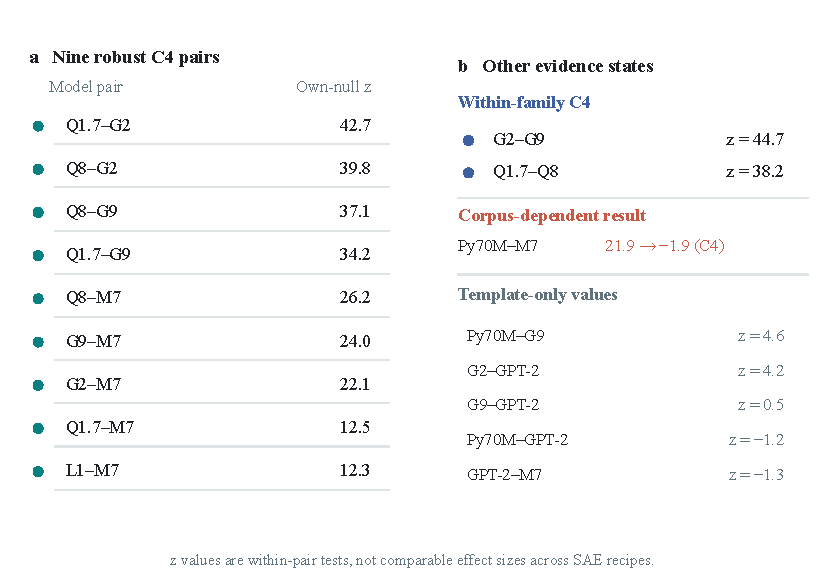
\includegraphics[width=1.0000\textwidth]{figures/integrated_20260923/fig04_redrawn.pdf}
\caption{\textbf{Evidence categories across model pairs.} The nine cross-family C4 pairs exceed their own permutation nulls. Exact z values are listed without a common magnitude color scale, because SAE recipes differ. The right panel preserves within-family controls, the template-to-C4 failure of Pythia-70M/Mistral, and all five template-only pairs. Low-count natural-text GPT-2 evaluations remain without a verdict; template z values must not be read as a natural-text result. Each unordered pair appears once.}
\label{fig:cross_model_sae}
\vspace{-3mm}
\end{figure}

\begin{figure}[h]
\centering
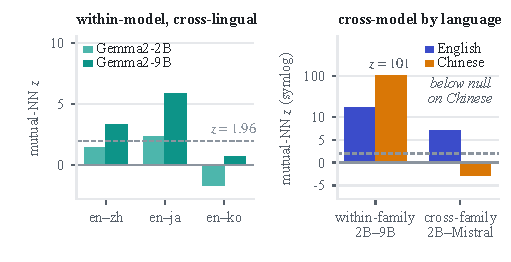
\includegraphics[width=0.62\textwidth]{figures/fig_language_panel.pdf}
\caption{\textbf{Cross-lingual sharing is weak within models and language-conditional
across them} (companion to \Cref{fig:cross_model_sae}; numbers in \Cref{tab:xling_cells}).
Left: within-model sharing clears the significance line for en--ja/en--zh in the
larger Gemma and, marginally, for en--ja in the smaller (nominal $z=2.3$, not
multiplicity-robust); en--ko is null in both. Right (symlog $y$): on Chinese, the within-family
pair shares strongly (shared tokenizer/script pipeline, flagged) while the cross-family
pair collapses below null despite sharing on English. Plotted from the
\texttt{xling\_*.json} and \texttt{zh\_gemma2-2b\_\_*.json} receipts.}
\label{fig:language_panel}
\end{figure}

\begin{table}[h]
\centering
\caption{\textbf{Cross-lingual and language-conditional cells with the validated tool}
(mutual-NN $z$ over the permutation null; $N=206$ aligned concepts unless noted; * $=$
permutation $p\leq0.05$). Left: \emph{within-model} en$\leftrightarrow$X feature sharing.
Right: cross-model cells by prompt language, plus the C4 natural-text control ($N=2000$)
and the $n_{\text{perm}}{=}2000$ hardening.}
\label{tab:xling_cells}
\small
\begin{tabular}{lrrr}
\toprule
Within-model & en--zh & en--ja & en--ko \\
\midrule
Gemma2-2B & $1.4$ & $2.3^{*}$ & $-1.7$ \\
Gemma2-9B & $3.3^{*}$ & $5.8^{*}$ & $0.7$ \\
\bottomrule
\end{tabular}
\hspace{1.2em}
\begin{tabular}{lrr}
\toprule
Cross-model & en & zh \\
\midrule
Gemma2-2B$\leftrightarrow$9B & $17.4^{*}$ & $101.0^{*}$ \\
Gemma2-2B$\leftrightarrow$Mistral & $6.9^{*}$ & $-2.7$ \\
\midrule
C4 control ($N{=}2000$) & \multicolumn{2}{c}{G2$\leftrightarrow$G9 $44.7^{*}$;\ \ G9$\leftrightarrow$M $24.0^{*}$;\ \ Py$\leftrightarrow$M $-1.9$ (fails)} \\
$n_{\text{perm}}{=}2000$ (templates, $N{=}206$) & \multicolumn{2}{c}{both headline pairs $p=1/2001$} \\
\bottomrule
\end{tabular}
\end{table}

\section{Audit of a published protocol (Lan et al.)}\label{app:lan}

To show that the two ingredients our method adds --- a permutation null strong enough to
absorb the pairing step, and a natural-text corpus control --- are not optional, we
re-implement the \citet{lan2024universal} statistic and apply our control battery to
\emph{it}. Their protocol: greedily pair features across two models by max activation
correlation, then measure SVCCA and RSA between the \emph{paired decoder-weight rows},
significance judged against a \emph{random-pairing} baseline. We reproduce the pairing and
similarity statistic, and separately add their filters (\Cref{app:lan_filters}); \Cref{tab:lan}
is the statistic without them. We run it on four of our
pairs --- a strong surviving pair (Gemma-2-9B$\leftrightarrow$Mistral-7B, mutual-NN
C4 $z=24.0$), a weak surviving pair (Qwen3-1.7B$\leftrightarrow$Mistral-7B, C4 $z=12.5$),
the corpus-artifact pair our C4 control rejects (Pythia-70M$\leftrightarrow$Mistral-7B,
C4 $z=-1.9$), and a null pair (GPT-2$\leftrightarrow$Mistral-7B, $z=-1.3$) --- on both the
templated corpus and C4, adding one control of our own: a \emph{permuted-pairing} null that
permutes the prompt rows before the greedy pairing, destroying genuine cross-model
correspondence while preserving the pairing step's opportunism (\Cref{tab:lan}).

\begin{table}[h]
\centering
\caption{\textbf{The Lan et al.\ protocol under our controls, without their filters} (with them:
\Cref{tab:lanfilt}). SVCCA and RSA of greedily
paired decoder spaces, with the original \emph{random}-pairing baseline and our stricter
\emph{permuted}-pairing null; ``exc.'' $=$ RSA $-$ permuted-null RSA. Three findings, each a
control our method supplies: (i) for the three non-null pairs the random-pairing baseline
sits far below the permuted-pairing null on both statistics --- RSA rand $\approx0$ vs.\
perm $0.041$--$0.150$, and SVCCA rand $0.164$--$0.167$ vs.\ perm $0.194$--$0.251$ --- so
the greedy pairing step itself manufactures $15$--$94\%$ of the RSA ``signal above random'' (least for
the strongest pair on C4, most on the templated corpus), while the
null pair shows no such gap (GPT-2 RSA perm $\approx0$); (ii) the
statistic is \emph{corpus-dependent} --- on the templated corpus even the strongest surviving
pair collapses to the artifact's level (exc.\ $+0.010$ both); (iii) on C4 it separates only
the \emph{strongest} pair ($+0.242$), while the weak surviving pair ($+0.079$) is
indistinguishable from the corpus artifact ($+0.068$) --- the artifact even scores higher on
raw RSA ($0.146$ vs.\ $0.134$). Only the null pair is correctly $\approx0$. Our
reciprocal-matching battery with a natural-text control separates the surviving pairs from the
corpus artifact and the null pair; it makes no strong-vs-weak ordering.}
\label{tab:lan}
\small
\setlength{\tabcolsep}{3pt}
\resizebox{\textwidth}{!}{%
\begin{tabular}{llrrrr rrr}
\toprule
& & \multicolumn{4}{c}{RSA} & \multicolumn{3}{c}{SVCCA} \\
\cmidrule(lr){3-6}\cmidrule(lr){7-9}
Pair (our verdict) & corpus & obs & rand & perm & exc. & obs & rand & perm \\
\midrule
Gemma-2-9B$\leftrightarrow$Mistral (survives, $z{=}24.0$) & templates & $0.161$ & $-0.001$ & $0.150$ & $+0.010$ & $0.258$ & $0.167$ & $0.209$ \\
 & C4 & $0.284$ & $-0.000$ & $0.041$ & $\mathbf{+0.242}$ & $0.457$ & $0.167$ & $0.194$ \\
\addlinespace
Qwen3-1.7B$\leftrightarrow$Mistral (survives, $z{=}12.5$) & templates & $0.099$ & $0.002$ & $0.063$ & $+0.036$ & $0.293$ & $0.167$ & $0.236$ \\
 & C4 & $0.134$ & $-0.001$ & $0.054$ & $+0.079$ & $0.387$ & $0.167$ & $0.219$ \\
\addlinespace
Pythia-70M$\leftrightarrow$Mistral (artifact, $z{=}{-}1.9$) & templates & $0.086$ & $0.003$ & $0.076$ & $+0.010$ & $0.288$ & $0.165$ & $0.251$ \\
 & C4 & $0.146$ & $0.000$ & $0.078$ & $+0.068$ & $0.350$ & $0.164$ & $0.236$ \\
\addlinespace
GPT-2$\leftrightarrow$Mistral (null, $z{=}{-}1.3$) & templates & $0.001$ & $0.000$ & $-0.001$ & $+0.002$ & $0.174$ & $0.168$ & $0.178$ \\
 & C4 & $0.000$ & $0.001$ & $-0.002$ & $+0.002$ & $0.190$ & $0.167$ & $0.187$ \\
\bottomrule
\end{tabular}}
\end{table}

The audit is not a claim that \citet{lan2024universal}'s within-scope finding is wrong ---
they compare same-tokenizer pairs, mostly within one family, and make a rotation-invariant
\emph{space}-level claim. It shows that their statistic, transplanted to the cross-family
regime without their filters, needs the two controls that let our reciprocal-matching battery
separate a real signal from a corpus artifact: a stricter-than-random null (their random
baseline is far too weak), and a natural-text corpus (on templates the statistic cannot even
separate the strongest genuine pair from the artifact). Their filters change the first two
findings and leave the third, by a narrow margin (\Cref{app:lan_filters}). The implementations
(\texttt{code/analysis/lan\_protocol\_audit.py} and \texttt{lan\_filter\_audit.py}, selftests
included) are in the code release.

\paragraph{The reverse transplant: their pairing rule inside our strongest control.}
\Cref{tab:lanpair} reports the complementary direction --- their 1A-to-ManyB pairing rule
substituted for our mutual-NN criterion inside the \Cref{tab:lextok} lexical-residualization
pipeline, everything else held fixed. Design, adequacy gate, tie rule (\emph{largest}
adequacy-passing $k$) and all five outcome branches were registered before any receipt
existed; the committed reader refuses partial input and applies the reimplementation
validity gate before reading any $R_{\text{lex}}$. Outcome: the registered survival branch,
$R_{\text{lex}}=0.900/0.905/0.910$ at governing $k{=}4096$, every $p$ at the $1/2001$ floor.
One $k$-dependence, disclosed rather than averaged away: the sign of the small gap between
their rule and ours is not stable across $k$ --- at $k{=}256$ their argmax pairs retain
marginally \emph{more} than our mutual-NN pairs, while at the governing $k{=}4096$ they
retain marginally less in all three cells. The registered readout is the largest
adequacy-passing $k$ (the strongest first stage), and we report that; the cross-$k$ receipts are
\texttt{lanpair\_lextok20k\_*\_k\{256,1024,4096\}.json}. The comparison
supports one claim only: survival under lexical residualization does not depend on which of
the two pairing rules is used. It licenses no ranking of the rules.

\begin{table}[h]
\centering
\caption{\textbf{The same control, applied to a published pairing rule.} \citet{lan2024universal} pair cross-model SAE features by taking, for each feature in $A$, its highest-correlated feature in $B$ (their 1A-to-ManyB rule; many-to-one by construction). We transplant \emph{that rule} into the \Cref{tab:lextok} pipeline and change nothing else --- same $20{,}000$ C4 documents, same cached pooled features, same TF-IDF$\to$SVD$_k$ cross-fitted design, same row-shuffled calibration, same within-fold null, $n_{\text{perm}}{=}2{,}000$. \emph{reimpl.}: the validity gate read \emph{before} any $R_{\text{lex}}$ --- the mapping must be many-to-one and its $1$--$1$ fraction must fall inside the $[0.159,0.632]$ interval implied by their Tables~5--6; it is necessary, not sufficient (an arbitrary argmax assignment gives $\approx 1/e$). \emph{ours}: the mutual-NN $R_{\text{lex}}$ from \Cref{tab:lextok} on the same cell. Receipts: \texttt{lanpair\_lextok20k\_*.json}.}
\label{tab:lanpair}
\footnotesize
\setlength{\tabcolsep}{4pt}
\begin{tabular}{llrrrrrrr}
\toprule
Cell & band & $k$ & pairs & $1$--$1$ frac & ret.\ real & ret.\ shuf & $R_{\text{lex}}$ & ours \\
\midrule
Qwen3-1.7B $\leftrightarrow$ Gemma2-2B & strong & $4096$ & $1500$ & $0.413$ & $0.899$ & $1.000$ & $0.900$ & $0.933$ \\
Gemma2-9B $\leftrightarrow$ Mistral-7B & median & $4096$ & $1500$ & $0.424$ & $0.904$ & $0.999$ & $0.905$ & $0.942$ \\
Llama-3.2-1B $\leftrightarrow$ Mistral-7B & weak & $4096$ & $1500$ & $0.299$ & $0.908$ & $0.998$ & $0.910$ & $0.918$ \\
\bottomrule
\end{tabular}
\end{table}


\paragraph{A third pairing rule: orthogonally aligned, fitted off the evaluation data.}
\citet{polymorphism_rotation2026} report that decoder-cosine similarity matches across
seeds at $98\%$ while an SAE trained on one seed reconstructs another's activations at
negative explained variance, and argue the standard universality metric cannot see that
failure. The account predicts something testable here: if the cross-model correspondence is
a rotation of a shared subspace, pairing in an orthogonally \emph{aligned} coordinate
system should recover it at least as well as raw correlation pairing. We registered that
baseline before implementing it (branches P1--P4, rank $64$, split seed $0$, both fixed a
priori) and ran it with a leakage control: the alignment is fitted over the shared document
axis on a random half of the corpus --- assuming no feature correspondence --- and the
frozen pairs are then scored, with the identical residualization, on the \emph{held-out}
half only. The committed reader checks that leakage constraint (evaluation $N$ must equal
the recorded held-out size, rank and seed must match the registration) before reading any
$R_{\text{lex}}$.

The registered branch P1 fired: $R_{\text{lex}}=0.928/0.920/0.885$ at the governing
$k{=}4096$ (\Cref{tab:proclex}), every cell above the $0.70$ survival bar and three times
the $0.30$ collapse bar, on half the documents. Survival under lexical residualization is
therefore a property of the shared structure under \emph{three} pairing rules --- our
reciprocal mutual-NN criterion, \citeauthor{lan2024universal}'s published argmax rule, and
an orthogonally aligned rule fitted off the evaluation data --- rather than of any one
matching criterion. Two bounds we state rather than bury: the aligned rule retains slightly
\emph{less} than mutual-NN in every cell ($0.928$ vs $0.933$, $0.920$ vs $0.942$, $0.885$ vs
$0.918$), so alignment does not improve on raw pairing here; and halving the corpus halves
the first stage's power, which is why the registration fixed the split in advance and
forbade enlarging the corpus if the adequacy gate had failed.

\begin{table}[h]
\centering
\caption{\textbf{The same control, under a Procrustes-aligned pairing fitted on a disjoint document half.} A rotation account of cross-model correspondence~\citep{polymorphism_rotation2026} predicts that pairing in an orthogonally aligned coordinate system should recover the correspondence at least as well as raw correlation pairing, and that the standard universality metric is blind to the failure it documents. We test that here: the alignment is fitted over the \emph{shared document axis} on a random half of the $20{,}000$ C4 documents ($Q=UV^\top$ from the SVD of $U_B^\top U_A$, rank $64$, split seed $0$, both fixed a priori), so no feature correspondence is assumed by the fit; pairs are mutual nearest neighbors by cosine in that aligned space; and every quantity below --- raw excess, residualization, null --- is computed on the \emph{held-out} half only. Everything else matches \Cref{tab:lextok}. \emph{ours}: the mutual-NN $R_{\text{lex}}$ on the same cell. Registered at \texttt{3be9b7d} with branches P1--P4 before the pairing existed; the selftest proves it collapses on purely lexical synthetic data and survives on a genuine shared latent. Receipts: \texttt{proclex\_lextok20k\_*.json}.}
\label{tab:proclex}
\footnotesize
\setlength{\tabcolsep}{4pt}
\begin{tabular}{llrrrrrr}
\toprule
Cell & band & $k$ & pairs & ret.\ real & ret.\ shuf & $R_{\text{lex}}$ & ours \\
\midrule
Qwen3-1.7B $\leftrightarrow$ Gemma2-2B & strong & $4096$ & $609$ & $0.928$ & $0.999$ & $0.928$ & $0.933$ \\
Gemma2-9B $\leftrightarrow$ Mistral-7B & median & $4096$ & $491$ & $0.920$ & $1.000$ & $0.920$ & $0.942$ \\
Llama-3.2-1B $\leftrightarrow$ Mistral-7B & weak & $4096$ & $335$ & $0.885$ & $1.000$ & $0.885$ & $0.918$ \\
\bottomrule
\end{tabular}
\end{table}


\subsection{Audit with their filtering steps}\label{app:lan_filters}
\Cref{tab:lan} scores all $512$ greedy pairs. \citet{lan2024universal} filter the pairs first
(their Sec.~3 and Apps.~A and K; the order and details come from their released code): a pair
is dropped if either feature's five highest-activating tokens include a non-concept token
(punctuation, whitespace, or a BOS/EOS/padding token), and is kept only if the two top-five
lists share a token string; a target that receives several source features keeps one pair;
pairs with activation correlation ${\le}0.1$ are dropped. We added these three steps to the
audit under a pre-registration written before any activation was extracted, which fixed the
decision rules and the sentence for every outcome
(\texttt{notes/PREREG\_lan\_filters\_20260924.md}). Two adaptations are forced by our setting.
Token strings are compared after stripping whitespace, because our pairs mix SentencePiece and
byte-level tokenizers; on raw strings no cell keeps more than $18$ pairs. The pairing still
correlates pooled documents, not tokens. The top-five tokens come from a fresh forward pass
over the same inputs (an Apple-silicon run, with Gemma-2-9B from the
ungated bf16 re-upload \texttt{unsloth/gemma-2-9b}, not checked bit-for-bit), which reproduces every unfiltered statistic of
\Cref{tab:lan} to within $0.013$. Our permuted-pairing null is pushed through all three
filters, so it faces the same selection as the observed pairs.

\Cref{tab:lanfilt} gives the result. The filters keep $17$--$32\%$ of the pairs on templates
and $4.5$--$7.6\%$ on C4; they report $20$--$30\%$ for pretrained SAEs. On C4, $260$ of
Mistral's $512$ pool features have punctuation, whitespace or BOS among their top five tokens. The
null pair keeps no pair on either corpus: every top activation of the GPT-2 features sits on a
prompt's first token, and no GPT-2 pair passes the keyword step. Read against the
three findings of \Cref{tab:lan}:
(i)~With their filters, the pairing-step inflation remains on templates, much reduced, but on C4
the filters leave too few permuted pairs to measure it. On C4 the filters discard
the permuted pairings: no permutation draw keeps the $21$ pairs SVCCA needs (median $7$--$10$
kept). On templates the permuted null still sits above their random baseline (RSA
$0.026$--$0.040$ vs.\ ${\approx}0$, in $126$--$197$ of $200$ draws), but that is now
$7.5$--$14.1\%$ of the signal above random instead of $63$--$94\%$. The inflation we report is
therefore a property of the unfiltered statistic; their full pipeline guards against it in
part, and on C4 it does so by discarding most pairs.
(ii)~With their filters the templated corpus does separate the strongest pair from the
artifact (exc.\ $0.370$ vs.\ $0.158$), so this finding does not hold for their full pipeline.
(iii)~On C4 the filtered statistic still does not separate the weak surviving pair from the
artifact. The two pairs' obs $-$ rand is $0.324$ vs.\ $0.174$, but with only $30$ and $23$
pairs left that gap ($0.150$) is just inside the pre-registered noise band ($0.164$), a marginal
call. The strongest pair stays
separated from both ($0.574$).
Under their text's one-to-one reading (drop every many-to-one target instead of keeping one),
the permuted null is not estimable in any cell. The filtered result is their filters applied to
our transplant, not a replication of their numbers: their token-level instance unit, their
RSA variant and their same-tokenizer model pairs are not reproduced.

% AUTO-GENERATED by code/analysis/lanfilt_summary.py -- DO NOT HAND-EDIT.
% Numbers formatted from results/cross_model_sae/lanfilt{T,C}_*__mistral7b.json (filtered["P"]).
\begin{table}[h]
\centering
\caption{\textbf{The Lan et al.\ protocol with their filters.} Primary pre-registered variant
(non-concept and shared-keyword filter on whitespace-stripped top-5 token strings, their
code's one-to-one step, $r{>}0.1$). kept $=$ pairs left of the $512$ greedy pairs. RSA of
the kept pairs' decoder rows (obs), their shuffle baseline within the kept pairs (rand, $200$
draws), and our permuted-pairing null pushed through all three filters (perm, $200$ draws;
n.e.\ $=$ fewer than half the draws keep the $21$ pairs SVCCA needs, with the number that do).
exc.\ $=$ obs $-$ perm; $^{\dagger}$obs $-$ rand where perm is n.e.\ (the pre-registered
fallback). share $=$ (perm $-$ rand)/(obs $-$ rand), the quantity that is $63$--$94\%$ on the
templated corpus without the filters (\Cref{tab:lan}). SVCCA is near its ceiling on so few
rows, so its random baseline rises as kept shrinks; it is shown, not read. Receipts:
\texttt{lanfilt\{T,C\}\_*.json}; pre-registration:
\texttt{notes/PREREG\_lan\_filters\_20260924.md}.}
\label{tab:lanfilt}
\small
\setlength{\tabcolsep}{3pt}
\resizebox{\textwidth}{!}{%
\begin{tabular}{llr rrrrr rr}
\toprule
& & & \multicolumn{5}{c}{RSA} & \multicolumn{2}{c}{SVCCA} \\
\cmidrule(lr){4-8}\cmidrule(lr){9-10}
Pair (our verdict) & corpus & kept & obs & rand & perm & exc. & share & obs & rand \\
\midrule
Gemma-2-9B$\leftrightarrow$Mistral (survives) & templates & $86$ & $0.402$ & $0.002$ & $0.032$ & $0.370$ & $7.5\%$ & $0.559$ & $0.420$ \\
 & C4 & $39$ & $0.576$ & $0.002$ & n.e.\ ($0/200$) & $0.574$$^{\dagger}$ & --- & $0.764$ & $0.654$ \\
\addlinespace
Qwen3-1.7B$\leftrightarrow$Mistral (survives) & templates & $149$ & $0.405$ & $0.000$ & $0.040$ & $0.365$ & $9.8\%$ & $0.505$ & $0.314$ \\
 & C4 & $30$ & $0.322$ & ${-}0.001$ & n.e.\ ($0/200$) & $0.324$$^{\dagger}$ & --- & $0.800$ & $0.768$ \\
\addlinespace
Pythia-70M$\leftrightarrow$Mistral (artifact) & templates & $164$ & $0.184$ & $0.000$ & $0.026$ & $0.158$ & $14.1\%$ & $0.419$ & $0.299$ \\
 & C4 & $23$ & $0.178$ & $0.004$ & n.e.\ ($0/200$) & $0.174$$^{\dagger}$ & --- & $0.941$ & $0.922$ \\
\addlinespace
GPT-2$\leftrightarrow$Mistral (null) & templates & $0$ & \multicolumn{7}{c}{no pair kept} \\
 & C4 & $0$ & \multicolumn{7}{c}{no pair kept} \\
\bottomrule
\end{tabular}}
\end{table}


\section{Loose-criterion confound scatter}\label{app:greedy_scatter}

\Cref{fig:greedy_scatter} plots the Finding-2 confound: the strict mutual-NN $z$ separates the
GPT-2 pairs from the rest (within-family and cross-modern pairs overlap), while the greedy-max excess saturates for most pairs (the low-sharing
Pythia rows excepted) and carries no discriminating information. The same statistic still reports $z=59$ on the Pythia-70M$\leftrightarrow$Mistral-7B C4 cell, whose reciprocal count is at null.

\begin{figure}[h]
\centering
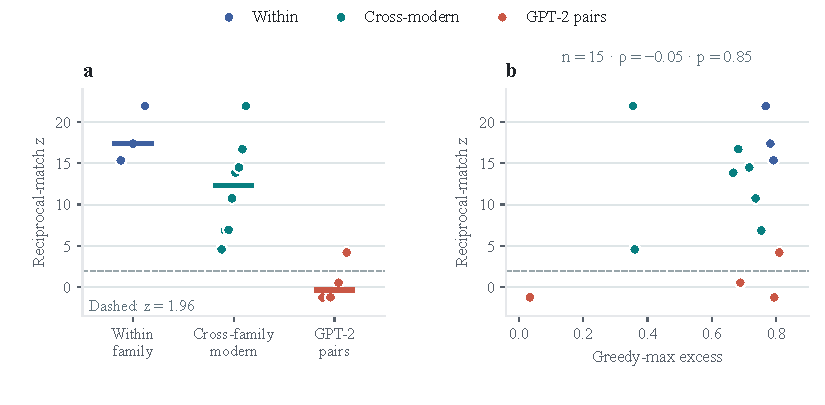
\includegraphics[width=1.0000\textwidth]{figures/integrated_20260923/fig06_redrawn.pdf}
\caption{\textbf{Pair classes overlap under the reciprocal statistic.} (a) Each point is a model pair and the thick mark the category median. Cross-modern pairs overlap within-family pairs. (b) The same 15 points against greedy-max excess: Spearman $\rho=-0.054$, $p=0.850$, so no monotonic association was detected in this sample. This is not proof of zero population association. Dashed lines denote nominal $z=1.96$; source: \texttt{results/cross\_model\_sae/SUMMARY.json}.}
\label{fig:greedy_scatter}
\end{figure}

\section{Zero-shot probe transfer: full detail}\label{app:probe_transfer}

A shared interface would carry an artifact across models: we
train a $9$-way concept-family
probe (closed-form ridge) on model A's matched-feature activations and apply it
\emph{unchanged} to model B's --- no training on the target, the unsupervised matching the
only shared coordinate
system; families are linearly separable within each model (CV${=}1.0$), so the test is
transfer vs.\ a \emph{non-matched} (permuted-matching) control. With the matching fit on the
same templated prompts used for evaluation, on all
three modern pairs the probe transfers zero-shot at $1.000$
($163$/$94$/$267$ matched features; controls $0.16$--$0.19$, $p=1/201$; majority-class rate $0.218$);
the null pair closes the loop (GPT-2$\leftrightarrow$Mistral: \emph{one} mutual-NN
feature; transfer $=$ control, $p=1.0$). Refit the matching on independent C4 text and transfer falls to chance ($0.12$--$0.20$,
$p{\geq}0.07$), so the in-sample transfer does not by itself establish a shared interface ---
Finding~1's corpus-conditionality at our own headline.

\section{Gemma Scope read point: a pre-registered sensitivity analysis}\label{app:gemmahook}
\paragraph{What was read.} In a Hugging Face forward pass \texttt{hidden\_states[$i$]} is the input to
block $i$. Gemma Scope's \texttt{layer\_$N$} dictionaries were trained on \texttt{resid\_post} of block
$N$, i.e.\ \texttt{hidden\_states[$N{+}1$]}; every Gemma cell in this paper applied them to
\texttt{hidden\_states[$N$]}, one block earlier ($N=12$ for Gemma-2-2B, $20$ for Gemma-2-9B). The cause
is our hook-index rule, which added one only when ``\texttt{resid\_post}'' appeared in the SAE's hook
name or id; under \texttt{sae-lens}~6 the hook name sits in the config's metadata and the Gemma Scope id
(\texttt{layer\_$N$/width\_16k/canonical}) does not contain it, so the shift never fired. The cluster
logs and receipts record index $N$ for every Gemma run. The other suites (Mistral, Qwen-Scope, Llama,
Pythia, GPT-2) are read at their own training hooks. Steering and ablation write at the same index,
so on the Gemma side they inject at our read point (\Cref{app:causal}).

\paragraph{Our read point is not the training point.} On the first $200$ C4 documents (BOS excluded),
the fraction of variance unexplained falls from our read point to the training hook for all three
Gemma dictionaries ($0.259\to0.172$ for 2B-16k, $0.248\to0.146$ for 2B-65k, $0.190\to0.156$ for 9B-16k)
and $L_0$ per token moves toward the release's nominal value ($74.8\to80.7$ vs.\ $82$; $67.1\to72.6$
vs.\ $72$; $47.9\to64.8$ vs.\ $68$). The features we report are therefore the released encoder
directions evaluated one block early, not the dictionaries on their training distribution, and the
feature labels in \Cref{app:matched-examples} are labels at our read point.

\paragraph{Registered sensitivity analysis.} Before any run we registered a re-run of the Gemma cells
of the C4 screen and the held-out confirmation in which the only change is reading
\texttt{hidden\_states[$N{+}1$]}; corpus, halves, top-$1{,}500$, permutations and seeds, and every
non-Gemma side are fixed (\texttt{notes/PREREG\_gemma\_hook\_sensitivity\_20260924.md}). Main-text
numbers stay at $N$ by that registration: every rung of a cell's ladder was computed at the same read
point, so each cell is internally consistent there. A cell is \emph{retained} at $N{+}1$ if its
held-out $p$ is $1/2001$, its held-out excess is positive and its screen $p\le1/201$. Two gates come
first: G0 (the re-run at $N$ reproduces the published receipt) and H (the fraction of variance
unexplained is lower and $L_0$ closer to nominal at $N{+}1$, the numbers above; H passes for all three
dictionaries). The Gemma-2-9B$\leftrightarrow$Mistral-7B numbers at $N{+}1$ had been seen during the
investigation that found the error, so that cell is reported but not counted. The registered
environment was Apple MPS with the ungated \texttt{unsloth} re-uploads of Gemma-2 (Google's repositories
are gated and were not available on that machine); the weights were not compared bit for bit, which is
what G0 checks. \emph{Deviation from the registration:} Qwen3-8B-Base could not be downloaded to that
machine, so the two Qwen3-8B cells were run on the cluster with Google's original weights, in the
environment that produced the published receipts; that run also repeated two other Gemma-2-9B cells,
which we report as a replication and do not use for any verdict.

\paragraph{Result (\Cref{tab:gemmahook}).} Registered outcome A (all retained, all in band): all four
blind cells that ran and passed the gates, Qwen3-1.7B$\leftrightarrow$Gemma-2-2B, Qwen3-8B$\leftrightarrow$Gemma-2-2B,
Qwen3-8B$\leftrightarrow$Gemma-2-9B and Gemma-2-2B$\leftrightarrow$Mistral-7B, are retained at the
training hook, with held-out excess moving by $-0.001$ to $+0.006$ and retained fraction by $-0.003$
to $+0.009$, inside the registered equivalence band ($\pm0.05$). Qwen3-1.7B$\leftrightarrow$Gemma-2-9B
missed G0 on the local run by one reciprocal pair ($\Delta M=3$ against a tolerance of $2$; its held-out
excess reproduced within $0.002$), so by the
registration it is not interpreted; in the cluster replication it passes G0 ($\Delta M=2$) and is
retained ($0.678\to0.679$, retained fraction $0.881\to0.892$). The non-blind
Gemma-2-9B$\leftrightarrow$Mistral-7B cell is retained and grows ($0.602\to0.617$, retained fraction
$0.791\to0.816$; cluster replication $0.615$ and $0.814$). The screen $z$ moves in both directions ($22.1\to19.0$ for
Gemma-2-2B$\leftrightarrow$Mistral-7B, $42.7\to45.0$ for Qwen3-1.7B$\leftrightarrow$Gemma-2-2B), which
is one more reason not to order cells by $z$ (\Cref{app:threats}). The width check keeps its
size: swapping the 16k for the 65k Gemma-2-2B dictionary moves the cell from $z=19.0$ to $10.9$ at
the training hook, against $22.1$ to $14.1$ at our read point.

\paragraph{Exploratory, not registered.} Re-running the top-document audit of
\Cref{app:matched-examples} for Gemma-2-9B$\leftrightarrow$Mistral-7B at the training hook leaves the
mean top-$5$ overlap of the top-$20$ pairs at $3.35/5$, and the obituary pair is still a reciprocal
match whose two features share all five top documents.

\paragraph{What this does not cover.} Only the pooled screen and held-out statistics were re-run,
and of the six cross-family Gemma cells only the four blind cells that passed G0 carry a registered
verdict. Everything else on the Gemma side stands at our read point: the control ladder (topic,
lexical and token-aligned arms, random dictionaries), the length- and coarse-topic-matched nulls,
the templated-corpus cells, the \citeauthor{lan2024universal} audit, the ablation probes, steering,
probe transfer and the cross-lingual Gemma cells. They are internally consistent there, and their
values at the training hook are untested.

\begin{table}[h]
\centering
\caption{\textbf{Gemma Scope cells read at the dictionaries' training hook} (pre-registered;
\Cref{app:gemmahook}). Each entry is $N$ / $N{+}1$: $N$ is the published value
(\texttt{hidden\_states[$N$]}, the input to block $N$; \Cref{tab:c4_counts,tab:c4_verdicts}),
$N{+}1$ reads \texttt{hidden\_states[$N{+}1$]}, the \texttt{resid\_post} hook each Gemma Scope
SAE was trained on, all else fixed. $z$: C4-screen mutual-NN $z$ ($200$ permutations); held-out
excess and retained fraction as in \Cref{tab:c4_verdicts} ($2{,}000$ permutations). G0: the
re-run at $N$ reproduces the published receipt (reciprocal count within $2$, held-out excess
within $0.005$). Verdict at $N{+}1$ by the registered rule (held-out $p=1/2001$, excess $>0$,
screen $p\le1/201$). Env: local = Apple MPS with ungated Gemma re-uploads; cluster = original
weights. $^{*}$Seen before registration; not counted. $^{\dagger}$Failed G0; not interpreted.
Receipts: \texttt{results/cross\_model\_sae/gemma\_hook\_sensitivity/}.}
\label{tab:gemmahook}
\scriptsize
\setlength{\tabcolsep}{2.5pt}
\begin{tabular}{llllllr}
\toprule
Cell & env & G0 & $z$ & held-out excess & retained & verdict at $N{+}1$ \\
\midrule
Qwen3-1.7B $\leftrightarrow$ Gemma2-2B & local & pass & $42.7$ / $45.0$ & $0.732$ / $0.731$ & $0.936$ / $0.932$ & retained \\
Qwen3-8B $\leftrightarrow$ Gemma2-2B & cluster & pass & $39.8$ / $35.8$ & $0.698$ / $0.704$ & $0.901$ / $0.908$ & retained \\
Qwen3-1.7B $\leftrightarrow$ Gemma2-9B & local & fail ($\Delta M{=}3$) & $34.2$ / $32.0$ & $0.678$ / $0.678$ & $0.881$ / $0.891$ & not interpreted$^{\dagger}$ \\
Qwen3-8B $\leftrightarrow$ Gemma2-9B & cluster & pass & $37.1$ / $38.1$ & $0.682$ / $0.686$ & $0.869$ / $0.878$ & retained \\
Gemma2-9B $\leftrightarrow$ Mistral-7B & local & pass & $24.0$ / $27.5$ & $0.602$ / $0.617$ & $0.791$ / $0.816$ & retained$^{*}$ \\
Gemma2-2B $\leftrightarrow$ Mistral-7B & local & pass & $22.1$ / $19.0$ & $0.567$ / $0.572$ & $0.818$ / $0.819$ & retained \\
\midrule
Gemma2-2B $\leftrightarrow$ Gemma2-9B & local & pass & $44.7$ / $44.5$ & -- & -- & screen only \\
Gemma2-2B(w$65$k) $\leftrightarrow$ Mistral-7B & local & pass & $14.1$ / $10.9$ & -- & -- & screen only \\
\bottomrule
\end{tabular}
\end{table}


\section{Extended threats to validity}\label{app:threats}

\paragraph{Scope caveats.} (i) GPT-2's four
natural-text cells are underpowered ($1$ reciprocal match vs.\ a null of ${\approx}2$),
so they support no verdict and GPT-2 is not a second below-threshold model --- exactly
one (Pythia-70M) is measured below its null with power --- and its
public SAE reads TransformerLens-processed activations \citep{nanda2022transformerlens};
(ii) cell $z$'s are not comparable across SAE recipes, so we claim no capability trend
and no convergence law; (iii) both ablation probes are inconclusive and no
cross-model causal intervention succeeded --- the functional evidence is within-model
steering transfer and in-sample zero-shot probe
transfer (\Cref{app:causal,app:probe_transfer}); (iv) every Gemma Scope dictionary was applied one
block before its training hook, so Gemma-side features, labels and steering are the released
directions at our read point, and only the pooled screen and held-out statistics were re-run at the
training hook (a pre-registered sensitivity analysis, \Cref{app:gemmahook}), for the six
cross-family Gemma cells: four blind cells are retained, the non-blind
Gemma-2-9B$\leftrightarrow$Mistral-7B cell is retained but not counted, and
Qwen3-1.7B$\leftrightarrow$Gemma-2-9B missed its reproduction gate on the registered run and is not
interpreted; nothing else on the Gemma side was re-run (the control ladder, the length- and
coarse-topic-matched nulls, the templated-corpus cells, the \citeauthor{lan2024universal} audit, the
ablation probes, steering, probe transfer and the cross-lingual Gemma cells; \Cref{app:gemmahook});
(v) the pooled feature averages over every token of a model's own tokenization, including a BOS
token where the tokenizer adds one. The BOS activation is identical across documents, so it enters
the pooled mean as $c_f/T_d$ ($c_f$ the feature's BOS activation, $T_d$ the document's token count),
a function of document length that two BOS-prepending models share. At the pinned revisions the
Gemma-2, Mistral-7B and Llama-3.2 tokenizers prepend BOS and the Qwen3-Base tokenizer does not
(tokenizers only; \texttt{code/analysis/bos\_probe\_ct.py}, \texttt{bos\_probe\_ct.json}), so in the six Qwen3 cells only one side
carries this term; that does not make those cells length-free, since the one-sided term can still
correlate with any length-sensitive feature of the other model. The shared route is open in the
three Gemma-2/Llama-3.2$\leftrightarrow$Mistral-7B cells. Length-decile nulls bound it in all three:
Gemma-2-2B$\leftrightarrow$Mistral-7B ($+14.6\%\to+14.3\%$ excess, \Cref{app:lencov}), and
Gemma-2-9B$\leftrightarrow$Mistral-7B and Llama-3.2-1B$\leftrightarrow$Mistral-7B, whose uncalibrated length arms keep
$0.993$ and $0.964$ of the excess (\Cref{app:ninecell}; after submission, calibrated length nulls cover all nine cells); the
token-aligned test excludes each document's first word and removes document means by construction;
the other held-out cells were not re-run without BOS, so we cannot say how much of their pooled excess
a length term carries. Recomputing the pooled features without position $0$ is the
direct check and is left to follow-up work;
(vi) no randomly initialized model was run through the pipeline. SAEs on such models can score
like trained ones on interpretability metrics \citep{heap2025random}, so the topical labels of
\Cref{app:matched-examples} are not by themselves evidence of learned features. The lexical and
word-type controls remove what unigram and current-word detectors share, not other structure two
random networks might share; a random-weight pair is the direct check and was not run.

\paragraph{External caveats on SAE matching.}
\emph{(i) Seed instability.} SAEs trained on the same data can learn different features
across seeds \citep{paulo2025sae}, even when the
underlying subspaces are stable \citep{gerasimov2026unstable}. Our matches use single
public releases per model, so cross-seed stability is untested. Three considerations bound
the damage. First, the direction of the bias: seed noise \emph{degrades} reciprocal
matching, and spurious matches are absorbed by the permutation null. Instability can shrink
the surviving-cell positive; the row-permutation null is conditional on the chosen SAE, so
it bounds rather than excludes recipe-induced alignment. Second, our claim is existential, not
one of per-feature identity. \emph{Some} matched set coactivates on the matching distribution; a
different seed finding a different set would not contradict that.
Third, the positive already spans four independently released SAE suites
(Gemma~Scope \citep{lieberum2024gemmascope}, a community Mistral SAE \citep{engels2024mistralsae}, Qwen-Scope \citep{qwenscope2026} via a manual loader, and a community Llama SAE \citep{chanind2024llamasae}), which makes a
shared-recipe explanation of the cross-suite matches unlikely.
A direct recipe check agrees on the \emph{verdict}. Swapping Gemma-2-2B's SAE for the
independently trained
width-$65$k release leaves the C4 cell significant (mutual-NN $473$ vs.\
permutation null $348$, $z=14.1$, $p=1/201$; $z=22.1$ at width $16$k). But the same check
bounds what may be read off the \emph{magnitude}: the width swap alone moves the cell by
$8.0$ in $z$ and $6.3$ points of excess with no change of model, corpus, or null
recipe. Since the nine surviving cells use four SAE suites at three released widths, cell $z$'s
are not on a common scale and no cross-cell ordering (in particular, no capability trend)
is claimed; the verdicts, being per-cell tests against per-cell nulls, are unaffected.

\emph{(i\,b) The GPT-2 cells are uninformative, not a second negative.} One might infer
GPT-2's sub-threshold status from the templated corpus --- the same corpus
Finding~1 shows can mis-estimate sharing in both directions. We therefore ran
all four GPT-2 cells on the identical $2{,}000$-document C4 slice, $\text{top-}k{=}1500$,
$n_{\text{perm}}{=}200$ configuration as the headline roster (\Cref{tab:gpt2_c4}). Every
cell is at or below its null ($z=-0.71$ to $-0.84$, $p=1.0$), but the test has essentially
no power there: GPT-2 yields \emph{one} reciprocal best-buddy pair against a permutation
null of ${\approx}2$, more than two orders of magnitude below the $348$--$553$ nulls of every other
cell. Whatever the cause --- the disclosed TransformerLens preprocessing of the
\texttt{gpt2-small-res-jb} release, the narrower $768$-dimensional residual, or genuinely
non-reciprocal structure --- a $1$-versus-$2$ comparison cannot distinguish ``no shared
features'' from ``the statistic does not resolve at this dictionary''. Note also that the
confounded greedy statistic reports $z=+5.5$ to $+46.0$ on these very cells, another
instance of Finding~2. We therefore do not read GPT-2 as a second below-threshold model:
exactly one model in this paper (Pythia-70M, $390$ observed vs.\ $411{\pm}11$ null) is
measured below its null on natural text at comparable power.

\begin{table}[h]
\centering
\caption{\textbf{GPT-2 natural-text cells.} Same C4 slice, top-$k$, and
$n_{\text{perm}}$ as \Cref{tab:c4_counts}; the Pythia row is repeated for scale. The GPT-2
nulls are ${\approx}2$ rather than ${\approx}400$, so these cells are underpowered, not
clean negatives. Receipts: \texttt{c4\_gpt2\_\_mistral7b.json},
\texttt{c4\_gemma2-2b\_\_gpt2.json}, \texttt{c4\_gemma2-9b\_\_gpt2.json},
\texttt{c4\_qwen3-1.7b\_\_gpt2.json} (JID 14851584).}
\label{tab:gpt2_c4}
\footnotesize
\setlength{\tabcolsep}{4pt}
\begin{tabular}{lrrrr}
\toprule
Cell & obs & null $\mu{\pm}\sigma$ & mutual $z$ & greedy $z$ \\
\midrule
GPT-2 $\leftrightarrow$ Mistral-7B     & $1$ & $2.0{\pm}1.4$ & $-0.76$ & $+5.5$ \\
Gemma2-2B $\leftrightarrow$ GPT-2      & $1$ & $2.1{\pm}1.3$ & $-0.84$ & $+46.0$ \\
Gemma2-9B $\leftrightarrow$ GPT-2      & $1$ & $1.9{\pm}1.2$ & $-0.79$ & $+42.6$ \\
Qwen3-1.7B $\leftrightarrow$ GPT-2     & $1$ & $2.0{\pm}1.4$ & $-0.71$ & $+37.4$ \\
\midrule
Pythia-70M $\leftrightarrow$ Mistral-7B (for scale) & $390$ & $411.1{\pm}10.9$ & $-1.93$ & $+59.2$ \\
\bottomrule
\end{tabular}
\end{table}

\emph{(ii) Matching score $\neq$ utility.} SAE interpretability scores correlate only weakly
with steering utility (Kendall $\tau_b\approx0.30$ across $90$ SAEs;
\citealp{wang2025interputility}), so a good matching score need not imply causal relevance
either. This is
why we accompany matching with causal, steering, and zero-shot transfer probes throughout.

\emph{(iii) Probe-transfer corpus scope.} The Finding-5 matching is fit \emph{label-free}
--- mutual-NN never sees the concept-family labels --- but on the same prompt distribution
used for probe evaluation. Given genuine co-activation, same-corpus transfer is then
expected to be high. The discriminating evidence is therefore the non-matched control
($\approx$chance, $p=1/201$) and the null pair, where the audited matching offers a single
feature and transfer collapses to the control. We ran the natural hardening: matching refit
on the independent $2{,}000$-document C4 slice, evaluation unchanged on the concept prompts.
It \emph{fails}. Transfer is $0.204/0.189/0.117$ on the three surviving pairs (controls
$0.10$--$0.16$, $p=0.07/0.35/0.62$; $K=123/125/63$ matched features), while the C4-matched
features remain concept-separable within each model (CV $0.91$--$0.99$) and the null pair
again yields a single feature (transfer $=$ control, $p=1.0$). The failure is stable:
refitting the matching on a held-out half of the C4 slice reproduces it on the headline
pair ($0.180$ vs.\ control $0.099$, $p=0.13$; $K=110$). The matched interface is
therefore \emph{corpus-bound}: matched features agree on the distribution that defined the
matching, but the correspondence does not transport concept geometry to a different prompt
distribution. This is the same corpus-conditionality that Finding~1 and the (unfiltered) protocol audit
(\Cref{app:lan}) document for the matching statistics themselves. All interface claims in
this paper are accordingly scoped to the matching distribution.

\emph{(iv) Selection and evaluation corpora.} Three designs, stated per layer so a reader
can see which claim rests on which. (1)~The nine discovery cells select pairs (top-$1{,}500$
features per side by variance, then reciprocal argmax) and compute their $200\times$
permutation null on the same $2{,}000$ C4 documents; but every null draw re-runs the argmax
on the permuted rows, so the reported excess is the count of reciprocal matches above the
chance level of \emph{re-selecting} under broken alignment, and no frozen pair set is
carried from selection to test (\texttt{cross\_model\_sae\_match.py},
\texttt{match\_and\_null}). The half-corpus refit (\texttt{c4h\_*.json}) repeats selection
and null on the second $1{,}000$ documents and reproduces every verdict; it is a stability
check, not a held-out evaluation. A held-out evaluation of frozen, A-selected pairs across
the full roster --- pairs selected on the first $1{,}000$ documents, scored on the disjoint
second $1{,}000$ with an evaluation-only null ($n_{\text{perm}}{=}2{,}000$;
\texttt{--select\_prompts} in \texttt{cross\_model\_sae\_match.py};
\texttt{run\_c4\_heldout\_frozen.sbatch}; \texttt{heldout\_*.json}) --- keeps every one of
the nine cells above its null: held-out pooled excess $0.52$--$0.73$, every $p$ at the
$1/2001$ floor, at $0.74$--$0.94$ of the in-sample excess re-selected on the evaluation
half itself (Qwen3$\leftrightarrow$Gemma-2 cells $0.87$--$0.94$, Mistral-7B cells
$0.74$--$0.82$; Llama-3.2-1B$\leftrightarrow$Mistral-7B lowest at $0.74$). On five of the cells,
seeded random halves in place of the consecutive ones change the median held-out excess by at most $3\%$
(\Cref{app:ninecell}; all nine cells after submission). The optimism
this design exposes ($6$--$26\%$) is larger than the $1$--$3\%$ of the split-half reported
below because selection and evaluation each see $1{,}000$ documents rather than
$10{,}000$ and only $42$--$75\%$ of the frozen pairs are re-selected on the evaluation
half; the two designs answer different questions and are not averaged. The one-cell
interpretability variant (Gemma-2-9B$\leftrightarrow$Mistral-7B, held-out pooled correlation
$0.69$, \texttt{interp\_heldout\_*.json}) is consistent with both. (2)~The fine-topic null
(\Cref{tab:covctl}) has the same construction as (1): each stratified draw re-selects. The
verdict-bearing lexical arm (\Cref{tab:lextok}) instead freezes the mutual-NN pairs computed
on the raw features of all $20{,}000$ documents and scores those pairs on cross-fitted
residuals of the same documents --- the cross-fitting is of the nuisance model, not of the
pair selection --- so selection enters both the raw and the residualized excess of
$R_{\text{lex}}$. We measured what that costs at the pooled level with a split-half on the
same three cells and the same registered seed-$42$ halves as the token-aligned rerun:
pairs selected on one $10{,}000$-document half and scored on the other, against an
evaluation-half-only null ($n_{\text{perm}}{=}2{,}000$), with the in-sample comparator
re-selecting on the evaluation half itself so both numbers sit on identical documents.
Held-out excess is $0.99/0.98/0.97$ of in-sample (Qwen3-1.7B$\leftrightarrow$Gemma-2-2B,
Gemma-2-9B$\leftrightarrow$Mistral-7B, Llama-3.2-1B$\leftrightarrow$Mistral-7B) (both directions averaged; every held-out
$p$ at the $1/2001$ floor; \texttt{splithalf20k\_*.json}, split SHA-256 identical to
\texttt{tokaclean20k\_*.json}), so same-corpus selection inflates the pooled excess by
$1$--$3\%$ in these cells. The registered Procrustes arm (\Cref{tab:proclex}) is the
disjoint-half version of the residualized test --- alignment and pairs fitted on one half;
raw excess, residualization and null on the other --- and survives in all three cells.
(3)~The token-aligned rerun is selection-clean by construction: a registered $50/50$
document split, candidate universe and reciprocal pairs computed on split~A only, every
statistic and every null draw on split-B occurrences only, with the split hashes and
requirement flags asserted in each \texttt{tokaclean20k\_*.json} receipt
(\Cref{app:tokalign}).

\paragraph{Shared-core control (pre-registered, unrun).}
We pre-registered a sharper test of whether the Qwen--Gemma probe-attribution gap is
mechanistic: restrict the correlation to each family's performance-recovering core
(ablate-and-measure) and re-test whether the gap persists (survives $\Rightarrow$ mechanistic;
collapses $\Rightarrow$ structural-surface effect). It is moot for the raw metric, which fails
construct validity (\Cref{sec:results:construct-validity}).


\paragraph{Scope of families, languages, and scaling endpoints.} The
\emph{probe-attribution} arm covers three families
(\qwen{}, \gemma{}, Pythia) and four languages (en/zh/ja/ko), and, after the construct-validity controls, it supports no cross-lingual claim. Its family roster is narrower
than the SAE-matching arm's because Llama/Mistral/DeepSeek have no
\circuittracer{}-compatible \emph{transcoders}; this is a constraint on the v0
attribution-graph route only, and Mistral-7B and Llama-3.2-1B carry released
\emph{SAEs} and are headline models in \Cref{sec:results:sae-matching}.
Within-family fits rest on few points (Qwen3
$n{=}5$, Gemma3/Pythia $n{=}4$), so slope CIs are wide. Caveats specific to the deferred v0
attribution-graph pipeline (backend OOM/convergence, identification assumptions, pruning
thresholds, backend asymmetry) are in \Cref{app:v0_limitations}.


\paragraph{Cross-model feature alignment (v0 only; superseded).} The v0 design would have
compared $\mathcal{F}(G_{\qwen{}})\cap
\mathcal{F}(G_{\gemma{}})$ as sets of $(\ell,f)$ tuples. That is only a heuristic --- feature
index $f$ in
\qwen{}'s transcoder is unrelated to feature index $f$ in \gemma{}'s, and layer indices are
relative to different $L$ --- and no such number is reported anywhere in this paper, because
the graphs never converged. The principled alternative (shared-prompt
activation correlation with a permutation null) \emph{is} the SAE-matching arm
of \Cref{sec:results:sae-matching}, which supersedes it.

\paragraph{Tokenizer and template confounds.} Cross-lingual overlap can be inflated or
deflated by tokenizer-level pre-features, which is why the v1 SAE arm mean-pools per prompt
(tokenizer-grid-free) and reports depth-banded cells. Prompt templates can also activate
genuinely different
circuits for the same task, so every cross-family cell fixes a single shared corpus across
models before comparing --- and \Cref{sec:results:sae-matching} shows the templated corpus
mis-estimates sharing in both directions, which is why the natural-text (C4) regime carries
the verdicts.

\paragraph{Pruning sensitivity and prompt-set size.} The $(\tau_n{=}0.8,\tau_e{=}0.98)$
thresholds match \circuittracer{} defaults. A threshold sweep was planned as a v0 robustness
check but is \emph{not applicable}: the v0 backend never converged (\Cref{app:robustness}),
so no threshold-sensitivity verification exists and none is claimed. The v0 plan used prompt
sets of 8--16 per family; no v0 result is reported.

\section{Methods for the v0 failure regime}\label{app:failure_methods}

In our v0 setup (\circuittracer{} v0.4.1 on the \texttt{nnsight} backend at float16,
\Cref{tab:hyperparams}), the attribution graphs of \citet{ameisen2025attribution} did not converge
on multistep and hallucination prompts at any Qwen3 size from 0.6B to 8B
($\tau\in\{10^{-2},10^{-3}\}$), even though the model answers these prompts correctly. The
library documents \texttt{nnsight} as experimental and uses TransformerLens by default; we did
not run that reference configuration on these prompts, so this is a failure of our pipeline, not
evidence that the method cannot recover these circuits. Any universality claim built on such a
pipeline must report per-task convergence and partition claims by whether the graph could be
recovered; \Cref{fig:pipeline} marks this deferred branch. Candidate substitutes (activation patching, SAE-feature sparse
regression, thinking-mode rollouts, natural-language autoencoders, dedicated feature
crosscoders for the cross-family arm) are surveyed below.

Beyond the per-task-convergence reporting recommended in \Cref{sec:disc:negative}, several
methods sidestep the attribution-graph convergence failure on multistep and
hallucination prompts. Activation patching \citep{heimersheim2024patching,
syed2023attribution} carries different but well-understood pitfalls and does not require
graph convergence; SAE-feature sparse regression bypasses the graph at the cost of
edge-level structure; thinking-mode rollouts reduce a 2-hop-per-prompt problem to a
1-hop-per-token one. Natural-language autoencoders \citep{nla2026anthropic} pair an
activation verbalizer with a reconstructor (0.6--0.8 FVE on Claude Opus 4.6 / Haiku
3.5/4.5), producing text-level descriptions rather than node-and-edge graphs; their finding
that multi-token claims are more factually accurate than single-token ones offers a
heuristic for the hallucination half of the failure regime. For the cross-family arm, the
Dedicated Feature Crosscoder of \citet{diff_tool2026anthropic} separates shared from
model-exclusive features across heterogeneous architectures (Llama-3.1-8B / Qwen3-8B /
GPT-OSS-20B / DeepSeek-R1-0528-Qwen3-8B), the principled shared/exclusive
decomposition the abandoned v0 Jaccard alignment only approximated. A learned shared dictionary
is not a drop-in replacement for our test: its shared latents are fit on the documents they would
then be scored on, so a null that re-runs that selection, as \Cref{prop:null}(b) requires, would
have to retrain the crosscoder in every permutation draw; we therefore compare released per-model SAEs. Agentic
interpretability --- an iterate-hypothesis-then-test loop that proposes method substitutions
automatically --- is a natural wrapper, with our negative-finding prompt set as a benchmark
on which to score whether a procedure recovers circuits our fixed attribution pass did not.

\section{Limitations specific to the v0 attribution-graph pipeline}\label{app:v0_limitations}

\paragraph{v0 backend OOM --- partially resolved.} The 121\,GiB CUDA OOM that blocked the v0
attribution-graph build at Qwen3-1.7B was root-caused: \texttt{compute\_score} in
\texttt{circuit\_tracer/attribution/context\_nnsight.py} allocated a full-batch
dtype-converted copy of the (batch, position, $d_\text{model}$) gradient tensor when
grads-dtype differed from output-vecs-dtype. Our batch-chunked patch
($\texttt{BATCH\_CHUNK}=4$) reduces peak memory from $O(B\cdot P\cdot D)$ to
$O(\text{CHUNK}\cdot P\cdot D)$, eliminating the OOM at Qwen3-0.6B (JID 8751067). At
Qwen3-1.7B the same chunk re-encountered the OOM on $7/8$ prompts (JID 9003117) despite
$139.8$\,GiB capacity --- a numerical-scaling artifact ($\texttt{BATCH\_CHUNK}$ must scale
inversely with model size), not a different bug. The iterative
\texttt{compute\_partial\_influences} convergence failure persists as a \emph{separate}
algorithmic issue, so the v0 negative-result framing is unchanged: our pipeline does not recover circuits
(zero valid \texttt{structure\_features}; \Cref{app:deferred}) because the
influence-propagation fixed point does not converge, not because of memory.

\paragraph{Other v0 caveats.} (i) \emph{Concept-grouping is hard-coded} to a small fixed set
(antonym, capital-city, $\dots$); auto-clustering by target-token semantic class was judged
not worth the engineering cost at this stage. (ii) \emph{One pruning threshold throughout}
keeps results comparable; the planned $(\tau_n,\tau_e)$ frontier was not run because the v0 backend never converged (\Cref{app:robustness}).
(iii) \emph{No causal verification of the cross-lingual claim}: we would report Jaccard
overlap, not interventions confirming that ablating a shared feature damages both languages.
(iv) \emph{Backend}: every v0 run, \qwen{} included, used the \texttt{nnsight} backend (the run
logs record it), which the library documents as experimental, slower and less memory-efficient
than its default TransformerLens backend; \gemma{}-PLT transcoders require \texttt{nnsight}. The
default backend was not tested on \qwen{}, so the non-convergence may be specific to our backend
and precision choices.

\paragraph{Identification assumptions.} Our attribution-graph results would rest on four
explicit assumptions, each testable: (a) \emph{faithful sparse-replacement} (the transcoder
reconstructs the residual contribution well enough that ablating features approximates
ablating the dense direction; gated by the library's $L_2$ reconstruction-error check); (b)
\emph{linear logit-lens identifiability} (per-layer activations decode to the target token
through the model's own unembedding --- what makes the v1 probe path well-defined where the
graph fails); (c) \emph{cross-language semantic alignment} (aligned en/zh/ja/ko pairs refer
to the same concept, controlled by a non-aligned shuffle baseline); (d) \emph{scale-invariant
pruning thresholds} (a fixed $(\tau_n,\tau_e)$ across the Qwen3 0.6B--8B family; failure-to-
converge is robust at $\tau\in\{10^{-2},10^{-3}\}$). We do \emph{not} assume the attribution
graph is the unique causal account: activation patching and probe-based logit-lens can give
different but compatible accounts.

\section{Full attribution-graph method}\label{app:method_full}

We adopt the attribution-graph formulation of \citet{ameisen2025attribution}. Given a frozen
base model $M$ with parameters $\theta$, pretrained transcoders
$\mathcal{T}=\{T_\ell\}_{\ell=1}^{L}$ replacing the MLP at each layer, and a prompt
$x=(x_1,\dots,x_n)$, we construct a directed graph $G(x;M,\mathcal{T})=(V,E)$ whose nodes
partition into \emph{feature nodes} $\{(\ell,p,f):a_{\ell,p,f}>0\}$, \emph{error nodes}
$\{(\ell,p)_{\text{err}}\}$, \emph{token nodes} $\{p_\text{tok}\}$, and \emph{logit nodes}
$\{(p_\text{logit},v)\}$. Edge weights $W_{ij}$ quantify the linearized direct effect of
source $j$ on target $i$; the dense adjacency is pruned via cumulative-influence thresholds
$(\tau_n,\tau_e)$ as in \citet{ameisen2025attribution}, with $\tau_n=0.8,\tau_e=0.98$
following the \circuittracer{} CLI defaults.

For two graphs we extract position-invariant feature identifiers
$\mathcal{F}(G)=\{(\ell,f):(\ell,p,f)\in V_G,\ \text{kind}=\text{feature}\}$ and report the
Jaccard similarity. Position invariance is necessary because aligned multilingual prompts
have different token lengths; for cross-model comparisons $\mathcal{F}$ uses model-relative
layer indices but matched prompt sets. Per pruned graph we also compute $|V|,|E|$, density
$|E|/(|V|(|V|-1))$, layer-span, edge-weight moments $(\bar w,\sigma_w,w_{\max})$, and mean
in/out-degree.

To validate causal involvement we use \circuittracer{}'s \texttt{feature\_intervention}
hook: given $(\ell,p,f,v)$ it clamps $a_{\ell,p,f}:=v$ and re-runs the forward pass,
reporting $\Delta_v=\log p_v(\text{intervened})-\log p_v(\text{baseline})$ and the perturbed
top-5 set. We use \circuittracer{} (\texttt{safety-research/circuit-tracer}) with the
\texttt{nnsight} backend for both families (our configuration default; required by
\gemma{}-PLT transcoders), \texttt{float16} weights, backward $\text{batch\_size}=256$, and
\texttt{lazy\_decoder} to fit \gemma{12B} on one A100 (v0 attribution-graph runs only). Hyperparameters are in
\Cref{tab:hyperparams}.

\section{Ethics Statement}
This work uses public language models and public corpora, involves no human
subjects and no personal data, and makes no deployment claim. Cross-model
feature-sharing claims are used to argue that interpretability findings transfer
between models, which would license auditing one model by proxy for another. The
ethical risk is that such transfer is asserted from a correlation that a control
would have removed. We therefore report the result only after an escalating
series of controls built to kill it, name the three artifacts that did not
survive those controls, and scope the surviving claim to the cells where it was
measured.

\section{AI Use Disclosure}\label{app:ai}

We used generative AI tools (Anthropic Claude and OpenAI Codex agents) to implement experiment code
and check it for correctness, to collect public datasets, to check references, and to polish the
writing. The authors take full responsibility for all content.


\end{document}
